\documentclass[twoside]{book}

% Packages required by doxygen
\usepackage{fixltx2e}
\usepackage{calc}
\usepackage{doxygen}
\usepackage[export]{adjustbox} % also loads graphicx
\usepackage{graphicx}
\usepackage[utf8]{inputenc}
\usepackage{makeidx}
\usepackage{multicol}
\usepackage{multirow}
\PassOptionsToPackage{warn}{textcomp}
\usepackage{textcomp}
\usepackage[nointegrals]{wasysym}
\usepackage[table]{xcolor}

% Font selection
\usepackage[T1]{fontenc}
\usepackage[scaled=.90]{helvet}
\usepackage{courier}
\usepackage{amssymb}
\usepackage{sectsty}
\renewcommand{\familydefault}{\sfdefault}
\allsectionsfont{%
  \fontseries{bc}\selectfont%
  \color{darkgray}%
}
\renewcommand{\DoxyLabelFont}{%
  \fontseries{bc}\selectfont%
  \color{darkgray}%
}
\newcommand{\+}{\discretionary{\mbox{\scriptsize$\hookleftarrow$}}{}{}}

% Page & text layout
\usepackage{geometry}
\geometry{%
  a4paper,%
  top=2.5cm,%
  bottom=2.5cm,%
  left=2.5cm,%
  right=2.5cm%
}
\tolerance=750
\hfuzz=15pt
\hbadness=750
\setlength{\emergencystretch}{15pt}
\setlength{\parindent}{0cm}
\setlength{\parskip}{0.2cm}
\makeatletter
\renewcommand{\paragraph}{%
  \@startsection{paragraph}{4}{0ex}{-1.0ex}{1.0ex}{%
    \normalfont\normalsize\bfseries\SS@parafont%
  }%
}
\renewcommand{\subparagraph}{%
  \@startsection{subparagraph}{5}{0ex}{-1.0ex}{1.0ex}{%
    \normalfont\normalsize\bfseries\SS@subparafont%
  }%
}
\makeatother

% Headers & footers
\usepackage{fancyhdr}
\pagestyle{fancyplain}
\fancyhead[LE]{\fancyplain{}{\bfseries\thepage}}
\fancyhead[CE]{\fancyplain{}{}}
\fancyhead[RE]{\fancyplain{}{\bfseries\leftmark}}
\fancyhead[LO]{\fancyplain{}{\bfseries\rightmark}}
\fancyhead[CO]{\fancyplain{}{}}
\fancyhead[RO]{\fancyplain{}{\bfseries\thepage}}
\fancyfoot[LE]{\fancyplain{}{}}
\fancyfoot[CE]{\fancyplain{}{}}
\fancyfoot[RE]{\fancyplain{}{\bfseries\scriptsize Generated on Tue Nov 8 2016 19\+:35\+:02 for C\+E\+C F\+R\+A\+M\+E\+W\+O\+R\+K by Doxygen }}
\fancyfoot[LO]{\fancyplain{}{\bfseries\scriptsize Generated on Tue Nov 8 2016 19\+:35\+:02 for C\+E\+C F\+R\+A\+M\+E\+W\+O\+R\+K by Doxygen }}
\fancyfoot[CO]{\fancyplain{}{}}
\fancyfoot[RO]{\fancyplain{}{}}
\renewcommand{\footrulewidth}{0.4pt}
\renewcommand{\chaptermark}[1]{%
  \markboth{#1}{}%
}
\renewcommand{\sectionmark}[1]{%
  \markright{\thesection\ #1}%
}

% Indices & bibliography
\usepackage{natbib}
\usepackage[titles]{tocloft}
\setcounter{tocdepth}{3}
\setcounter{secnumdepth}{5}
\makeindex

% Hyperlinks (required, but should be loaded last)
\usepackage{ifpdf}
\ifpdf
  \usepackage[pdftex,pagebackref=true]{hyperref}
\else
  \usepackage[ps2pdf,pagebackref=true]{hyperref}
\fi
\hypersetup{%
  colorlinks=true,%
  linkcolor=blue,%
  citecolor=blue,%
  unicode%
}

% Custom commands
\newcommand{\clearemptydoublepage}{%
  \newpage{\pagestyle{empty}\cleardoublepage}%
}


%===== C O N T E N T S =====

\begin{document}

% Titlepage & ToC
\hypersetup{pageanchor=false,
             bookmarks=true,
             bookmarksnumbered=true,
             pdfencoding=unicode
            }
\pagenumbering{roman}
\begin{titlepage}
\vspace*{7cm}
\begin{center}%
{\Large C\+E\+C F\+R\+A\+M\+E\+W\+O\+R\+K \\[1ex]\large 0.\+0.\+1 }\\
\vspace*{1cm}
{\large Generated by Doxygen 1.8.9.1}\\
\vspace*{0.5cm}
{\small Tue Nov 8 2016 19:35:02}\\
\end{center}
\end{titlepage}
\clearemptydoublepage
\tableofcontents
\clearemptydoublepage
\pagenumbering{arabic}
\hypersetup{pageanchor=true}

%--- Begin generated contents ---
\chapter{Cloud Edge Computing(C\+E\+C) framework}
\label{index}\hypertarget{index}{}Written by ysmoon 
\chapter{Todo List}
\label{todo}
\hypertarget{todo}{}

\begin{DoxyRefList}
\item[\label{todo__todo000001}%
\hypertarget{todo__todo000001}{}%
Class \hyperlink{classDESTCELL}{D\+E\+S\+T\+C\+E\+L\+L} ]D\+B로 보내기, src cell에 연결되지 않은 device도 연결을 받아 보내기  
\item[\label{todo__todo000002}%
\hypertarget{todo__todo000002}{}%
Member \hyperlink{classFACTORYBUILDER_ad29f6bcb828945d37bee154b247ded10}{F\+A\+C\+T\+O\+R\+Y\+B\+U\+I\+L\+D\+E\+R\+:\+:make\+B\+A\+S\+I\+C\+C\+E\+L\+L} (int count, F\+U\+N\+C func, \hyperlink{classSTREAMFACTORY}{S\+T\+R\+E\+A\+M\+F\+A\+C\+T\+O\+R\+Y} $\ast$streamfactory)]processing rate와 튜플당 처리되야 하는 deadline을 정할 수 있는 파라미터 도입 예정 \begin{DoxyReturn}{Returns}
생성된 베이직 셀의 객체 포인터  
\end{DoxyReturn}

\item[\label{todo__todo000005}%
\hypertarget{todo__todo000005}{}%
Member \hyperlink{classFACTORYBUILDER_ab56a2ef6e49fa0370c3b1138e2350d01}{F\+A\+C\+T\+O\+R\+Y\+B\+U\+I\+L\+D\+E\+R\+:\+:make\+D\+E\+S\+T\+C\+E\+L\+L} (\hyperlink{classSTREAMFACTORY}{S\+T\+R\+E\+A\+M\+F\+A\+C\+T\+O\+R\+Y} $\ast$streamfactory)]추후 D\+B과의 출력을 담당할 예정이다.  
\item[\label{todo__todo000004}%
\hypertarget{todo__todo000004}{}%
Member \hyperlink{classFACTORYBUILDER_a1378efcb11e24157cfbdb325e9cbaf2b}{F\+A\+C\+T\+O\+R\+Y\+B\+U\+I\+L\+D\+E\+R\+:\+:make\+S\+R\+C\+C\+E\+L\+L} (int recvport, \hyperlink{classSTREAMFACTORY}{S\+T\+R\+E\+A\+M\+F\+A\+C\+T\+O\+R\+Y} $\ast$streamfactory)]추후 D\+B등과의 입력을 담당할 예정이다.  
\item[\label{todo__todo000003}%
\hypertarget{todo__todo000003}{}%
Member \hyperlink{classFACTORYBUILDER_a485976fa00bdee0a822ef949c3db31e0}{F\+A\+C\+T\+O\+R\+Y\+B\+U\+I\+L\+D\+E\+R\+:\+:make\+U\+N\+I\+O\+N\+C\+E\+L\+L} (int cellid, int count, \hyperlink{classSTREAMFACTORY}{S\+T\+R\+E\+A\+M\+F\+A\+C\+T\+O\+R\+Y} $\ast$streamfactory, int policy)]processing rate와 튜플당 처리되야 하는 deadline을 정할 수 있는 파라미터 도입 예정 \begin{DoxyReturn}{Returns}
생성된 유니언 셀의 객체 포인터  
\end{DoxyReturn}

\item[\label{todo__todo000006}%
\hypertarget{todo__todo000006}{}%
Member \hyperlink{classTUPLE_ac92a492d3f8a793fe02fe364244c34af}{T\+U\+P\+L\+E\+:\+:T\+U\+P\+L\+E} (char $\ast$packet, bool is\+Special)]is\+Special이 false인경우 프로그램이 종료된다. (미구현)  
\item[\label{todo__todo000007}%
\hypertarget{todo__todo000007}{}%
Member \hyperlink{classUNIONCELL_a42d955ed8ce559f41bd4837eda14a4ee}{U\+N\+I\+O\+N\+C\+E\+L\+L\+:\+:getpipelock} ()]pipe락을 없애는 방법이 있으면 없애기 
\end{DoxyRefList}
\chapter{Bug List}
\label{bug}
\hypertarget{bug}{}

\begin{DoxyRefList}
\item[\label{bug__bug000001}%
\hypertarget{bug__bug000001}{}%
Member \hyperlink{classBASICCELL_a2e910313cdad1651908cca08f89be64c}{B\+A\+S\+I\+C\+C\+E\+L\+L\+:\+:scheduling} (void $\ast$arg)]스케줄링에서 outpipe로 데이터를 넘길 때, pipe에 각각 데이터를 깊은복사를 해서 넘겨주어야 한다.  
\item[\label{bug__bug000002}%
\hypertarget{bug__bug000002}{}%
Member \hyperlink{classUNIONCELL_a0179dad91d30e7bca318bb7e3b4a4995}{U\+N\+I\+O\+N\+C\+E\+L\+L\+:\+:scheduling} (void $\ast$arg)]스케줄링에서 outpipe로 데이터를 넘길 때, pipe에 각각 데이터를 깊은복사를 해서 넘겨주어야 한다. 
\end{DoxyRefList}
\chapter{Hierarchical Index}
\section{Class Hierarchy}
This inheritance list is sorted roughly, but not completely, alphabetically\+:\begin{DoxyCompactList}
\item \contentsline{section}{C\+E\+L\+L}{\pageref{classCELL}}{}
\begin{DoxyCompactList}
\item \contentsline{section}{B\+A\+S\+I\+C\+C\+E\+L\+L}{\pageref{classBASICCELL}}{}
\item \contentsline{section}{D\+E\+S\+T\+C\+E\+L\+L}{\pageref{classDESTCELL}}{}
\item \contentsline{section}{S\+R\+C\+C\+E\+L\+L}{\pageref{classSRCCELL}}{}
\item \contentsline{section}{U\+N\+I\+O\+N\+C\+E\+L\+L}{\pageref{classUNIONCELL}}{}
\end{DoxyCompactList}
\item \contentsline{section}{C\+L\+I\+E\+N\+T}{\pageref{structCLIENT}}{}
\item \contentsline{section}{C\+O\+N\+N\+D\+A\+T\+A}{\pageref{structCONNDATA}}{}
\item \contentsline{section}{C\+O\+N\+N\+E\+C\+T\+I\+O\+N}{\pageref{classCONNECTION}}{}
\item \contentsline{section}{F\+A\+C\+T\+O\+R\+Y\+B\+U\+I\+L\+D\+E\+R}{\pageref{classFACTORYBUILDER}}{}
\item \contentsline{section}{M\+I\+G\+R\+A\+T\+I\+O\+N}{\pageref{classMIGRATION}}{}
\item \contentsline{section}{P\+A\+C\+K\+E\+T}{\pageref{classPACKET}}{}
\item \contentsline{section}{P\+I\+P\+E}{\pageref{classPIPE}}{}
\item \contentsline{section}{S\+E\+R\+V\+E\+R}{\pageref{structSERVER}}{}
\item \contentsline{section}{S\+T\+R\+E\+A\+M\+F\+A\+C\+T\+O\+R\+Y}{\pageref{classSTREAMFACTORY}}{}
\item \contentsline{section}{T\+U\+P\+L\+E}{\pageref{classTUPLE}}{}
\item \contentsline{section}{W\+O\+R\+K\+E\+R}{\pageref{classWORKER}}{}
\end{DoxyCompactList}

\chapter{Class Index}
\section{Class List}
Here are the classes, structs, unions and interfaces with brief descriptions\+:\begin{DoxyCompactList}
\item\contentsline{section}{\hyperlink{classBASICCELL}{B\+A\+S\+I\+C\+C\+E\+L\+L} \\*Cell의 기본 형태를 상속하고 S\+I\+S\+O의 형태를 갖고 있는 processing cell. 실제 processing의 유닛이다 }{\pageref{classBASICCELL}}{}
\item\contentsline{section}{\hyperlink{classCELL}{C\+E\+L\+L} \\*Processing cell의 기본 구현이 들어있는 클래스 }{\pageref{classCELL}}{}
\item\contentsline{section}{\hyperlink{structCLIENT}{C\+L\+I\+E\+N\+T} }{\pageref{structCLIENT}}{}
\item\contentsline{section}{\hyperlink{structCONNDATA}{C\+O\+N\+N\+D\+A\+T\+A} }{\pageref{structCONNDATA}}{}
\item\contentsline{section}{\hyperlink{classCONNECTION}{C\+O\+N\+N\+E\+C\+T\+I\+O\+N} }{\pageref{classCONNECTION}}{}
\item\contentsline{section}{\hyperlink{classDESTCELL}{D\+E\+S\+T\+C\+E\+L\+L} \\*Destcell을 정의해놓은 클래스. factory에서 나가는 데이터의 종말 지점이다 }{\pageref{classDESTCELL}}{}
\item\contentsline{section}{\hyperlink{classFACTORYBUILDER}{F\+A\+C\+T\+O\+R\+Y\+B\+U\+I\+L\+D\+E\+R} \\*Factory builder를 만든다 }{\pageref{classFACTORYBUILDER}}{}
\item\contentsline{section}{\hyperlink{classMIGRATION}{M\+I\+G\+R\+A\+T\+I\+O\+N} }{\pageref{classMIGRATION}}{}
\item\contentsline{section}{\hyperlink{classPACKET}{P\+A\+C\+K\+E\+T} }{\pageref{classPACKET}}{}
\item\contentsline{section}{\hyperlink{classPIPE}{P\+I\+P\+E} }{\pageref{classPIPE}}{}
\item\contentsline{section}{\hyperlink{structSERVER}{S\+E\+R\+V\+E\+R} }{\pageref{structSERVER}}{}
\item\contentsline{section}{\hyperlink{classSRCCELL}{S\+R\+C\+C\+E\+L\+L} \\*Srccell을 정의해놓은 클래스. factory로 들어오는 데이터의 시작 지점이다. cell의 형태를 상속하며 S\+O의 형태를 갖는다 }{\pageref{classSRCCELL}}{}
\item\contentsline{section}{\hyperlink{classSTREAMFACTORY}{S\+T\+R\+E\+A\+M\+F\+A\+C\+T\+O\+R\+Y} }{\pageref{classSTREAMFACTORY}}{}
\item\contentsline{section}{\hyperlink{classTUPLE}{T\+U\+P\+L\+E} \\*Data의 교환단위인 tuple을 정의한 클래스이다 }{\pageref{classTUPLE}}{}
\item\contentsline{section}{\hyperlink{classUNIONCELL}{U\+N\+I\+O\+N\+C\+E\+L\+L} \\*Cell의 기본 형태를 상속하고 M\+I\+S\+O의 형태를 갖고 있는 union cell이다. (processing cell이 아니다.) M\+I\+S\+O의 형태를 갖는다 }{\pageref{classUNIONCELL}}{}
\item\contentsline{section}{\hyperlink{classWORKER}{W\+O\+R\+K\+E\+R} }{\pageref{classWORKER}}{}
\end{DoxyCompactList}

\chapter{File Index}
\section{File List}
Here is a list of all documented files with brief descriptions\+:\begin{DoxyCompactList}
\item\contentsline{section}{include/\hyperlink{BASICCELL_8h}{B\+A\+S\+I\+C\+C\+E\+L\+L.\+h} \\*Processing cell의 basic cell을 정의해놓은 헤더 }{\pageref{BASICCELL_8h}}{}
\item\contentsline{section}{include/\hyperlink{CELL_8h}{C\+E\+L\+L.\+h} \\*Processing cell의 기본단위인 cell의 기본 형태를 정의해놓은 헤더 }{\pageref{CELL_8h}}{}
\item\contentsline{section}{include/{\bfseries Debug.\+h} }{\pageref{Debug_8h}}{}
\item\contentsline{section}{include/\hyperlink{DESTCELL_8h}{D\+E\+S\+T\+C\+E\+L\+L.\+h} \\*Destcell을 정의해놓은 헤더 }{\pageref{DESTCELL_8h}}{}
\item\contentsline{section}{include/\hyperlink{FACTORYBUILDER_8h}{F\+A\+C\+T\+O\+R\+Y\+B\+U\+I\+L\+D\+E\+R.\+h} \\*Factory를 만드는 툴인 factorybuilder를 정의해놓은 헤더 }{\pageref{FACTORYBUILDER_8h}}{}
\item\contentsline{section}{include/{\bfseries Functions.\+h} }{\pageref{Functions_8h}}{}
\item\contentsline{section}{include/{\bfseries M\+I\+G\+R\+A\+T\+I\+O\+N.\+h} }{\pageref{MIGRATION_8h}}{}
\item\contentsline{section}{include/{\bfseries P\+A\+C\+K\+E\+T.\+h} }{\pageref{PACKET_8h}}{}
\item\contentsline{section}{include/{\bfseries P\+I\+P\+E.\+h} }{\pageref{PIPE_8h}}{}
\item\contentsline{section}{include/\hyperlink{SRCCELL_8h}{S\+R\+C\+C\+E\+L\+L.\+h} \\*Srccell을 정의해놓은 헤더 }{\pageref{SRCCELL_8h}}{}
\item\contentsline{section}{include/{\bfseries S\+T\+R\+E\+A\+M\+F\+A\+C\+T\+O\+R\+Y.\+h} }{\pageref{STREAMFACTORY_8h}}{}
\item\contentsline{section}{include/\hyperlink{TUPLE_8h}{T\+U\+P\+L\+E.\+h} \\*Data의 교환단위인 tuple을 정의해놓은 헤더 }{\pageref{TUPLE_8h}}{}
\item\contentsline{section}{include/{\bfseries Type.\+h} }{\pageref{Type_8h}}{}
\item\contentsline{section}{include/\hyperlink{UNIONCELL_8h}{U\+N\+I\+O\+N\+C\+E\+L\+L.\+h} \\*두개 이상의 tuple을 합쳐주는 cell }{\pageref{UNIONCELL_8h}}{}
\item\contentsline{section}{include/{\bfseries W\+O\+R\+K\+E\+R.\+h} }{\pageref{WORKER_8h}}{}
\item\contentsline{section}{srcbackup/{\bfseries C\+O\+N\+N\+E\+C\+T\+I\+O\+N.\+h} }{\pageref{CONNECTION_8h}}{}
\end{DoxyCompactList}

\chapter{Class Documentation}
\hypertarget{classBASICCELL}{}\section{B\+A\+S\+I\+C\+C\+E\+L\+L Class Reference}
\label{classBASICCELL}\index{B\+A\+S\+I\+C\+C\+E\+L\+L@{B\+A\+S\+I\+C\+C\+E\+L\+L}}


cell의 기본 형태를 상속하고 S\+I\+S\+O의 형태를 갖고 있는 processing cell. 실제 processing의 유닛이다.  




{\ttfamily \#include $<$B\+A\+S\+I\+C\+C\+E\+L\+L.\+h$>$}



Inheritance diagram for B\+A\+S\+I\+C\+C\+E\+L\+L\+:\nopagebreak
\begin{figure}[H]
\begin{center}
\leavevmode
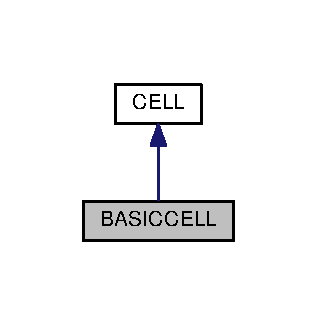
\includegraphics[width=152pt]{classBASICCELL__inherit__graph}
\end{center}
\end{figure}


Collaboration diagram for B\+A\+S\+I\+C\+C\+E\+L\+L\+:\nopagebreak
\begin{figure}[H]
\begin{center}
\leavevmode
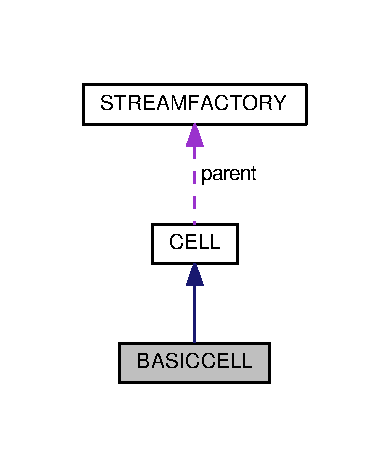
\includegraphics[width=187pt]{classBASICCELL__coll__graph}
\end{center}
\end{figure}
\subsection*{Public Member Functions}
\begin{DoxyCompactItemize}
\item 
\hyperlink{classBASICCELL_a0058bee3f5c99d05c321b47cb803badc}{B\+A\+S\+I\+C\+C\+E\+L\+L} (\hyperlink{classPIPE}{P\+I\+P\+E} $\ast$inpipe, \hyperlink{classPIPE}{P\+I\+P\+E} $\ast$outpipe, ushort count, F\+U\+N\+C func, \hyperlink{classSTREAMFACTORY}{S\+T\+R\+E\+A\+M\+F\+A\+C\+T\+O\+R\+Y} $\ast$parent)
\begin{DoxyCompactList}\small\item\em basiccell을 만드는 생성자 \end{DoxyCompactList}\item 
\hyperlink{classBASICCELL_a9e173d89e7c3c2b2513cb7f6d8f455b8}{B\+A\+S\+I\+C\+C\+E\+L\+L} (\hyperlink{classPIPE}{P\+I\+P\+E} $\ast$inpipe, list$<$ \hyperlink{classPIPE}{P\+I\+P\+E} $\ast$ $>$ $\ast$outpipelist, ushort count, F\+U\+N\+C func, \hyperlink{classSTREAMFACTORY}{S\+T\+R\+E\+A\+M\+F\+A\+C\+T\+O\+R\+Y} $\ast$parent)
\begin{DoxyCompactList}\small\item\em basiccell을 만드는 생성자 \end{DoxyCompactList}\item 
virtual void \hyperlink{classBASICCELL_aacb2fd7565d13f80e407854e0a978d73}{make\+Worker} ()
\begin{DoxyCompactList}\small\item\em 워커를 만든다. \end{DoxyCompactList}\item 
virtual void $\ast$ \hyperlink{classBASICCELL_a2e910313cdad1651908cca08f89be64c}{scheduling} (void $\ast$arg)
\begin{DoxyCompactList}\small\item\em 만든 워커를 실제로 스케줄링 하는 함수 \end{DoxyCompactList}\item 
\hyperlink{classPIPE}{P\+I\+P\+E} $\ast$ \hyperlink{classBASICCELL_a0008bc2d8bb7bd0f85729fd2f049458a}{getinpipe} ()
\begin{DoxyCompactList}\small\item\em 단일 inpipe를 반환하는 함수 \end{DoxyCompactList}\item 
F\+U\+N\+C \hyperlink{classBASICCELL_a0b157d23811cb140c2567572adc0034b}{getfunc} ()
\begin{DoxyCompactList}\small\item\em 코드 세그먼트를 반환하는 함수 \end{DoxyCompactList}\end{DoxyCompactItemize}
\subsection*{Additional Inherited Members}


\subsection{Detailed Description}
cell의 기본 형태를 상속하고 S\+I\+S\+O의 형태를 갖고 있는 processing cell. 실제 processing의 유닛이다. 

cell의 기본 형태를 상속하고 S\+I\+S\+O의 형태를 갖고 있는 processing cell. 실제 processing의 유닛이다. S\+I는 한번에 하나의 튜플만을 받음을 의미하며 이 튜플들은 독립적으로 처리된다. S\+O는 하나의 튜플만이 나오며 outpipe에는 데이터가 각각 복사된다. \begin{DoxyAuthor}{Author}
ysmoon 
\end{DoxyAuthor}
\begin{DoxyDate}{Date}
2016-\/11-\/08 
\end{DoxyDate}
\begin{DoxyVersion}{Version}
0.\+0.\+1 
\end{DoxyVersion}


\subsection{Constructor \& Destructor Documentation}
\hypertarget{classBASICCELL_a0058bee3f5c99d05c321b47cb803badc}{}\index{B\+A\+S\+I\+C\+C\+E\+L\+L@{B\+A\+S\+I\+C\+C\+E\+L\+L}!B\+A\+S\+I\+C\+C\+E\+L\+L@{B\+A\+S\+I\+C\+C\+E\+L\+L}}
\index{B\+A\+S\+I\+C\+C\+E\+L\+L@{B\+A\+S\+I\+C\+C\+E\+L\+L}!B\+A\+S\+I\+C\+C\+E\+L\+L@{B\+A\+S\+I\+C\+C\+E\+L\+L}}
\subsubsection[{B\+A\+S\+I\+C\+C\+E\+L\+L}]{\setlength{\rightskip}{0pt plus 5cm}B\+A\+S\+I\+C\+C\+E\+L\+L\+::\+B\+A\+S\+I\+C\+C\+E\+L\+L (
\begin{DoxyParamCaption}
\item[{{\bf P\+I\+P\+E} $\ast$}]{inpipe, }
\item[{{\bf P\+I\+P\+E} $\ast$}]{outpipe, }
\item[{ushort}]{count, }
\item[{F\+U\+N\+C}]{func, }
\item[{{\bf S\+T\+R\+E\+A\+M\+F\+A\+C\+T\+O\+R\+Y} $\ast$}]{parent}
\end{DoxyParamCaption}
)}\label{classBASICCELL_a0058bee3f5c99d05c321b47cb803badc}


basiccell을 만드는 생성자 

basiccell을 만드는 생성자. 
\begin{DoxyParams}{Parameters}
{\em inpipe} & cell에 대한 단일 input pipe이다. \\
\hline
{\em outpipe} & cell에 대한 단일 output pipe이다. \\
\hline
{\em count} & cell에 들어있는 worker의 개수를 정의한다. \\
\hline
{\em parent} & cell이 속한 factory를 명시한다. \\
\hline
{\em func} & 사용자가 정의할 수 있는 코드 세그먼트이다. T\+U\+P\+L\+E$\ast$ code(\+T\+U\+P\+L\+E$\ast$ tuple) 함수 형태를 갖는다. \\
\hline
{\em X\+I\+X\+O} & cell의 input과 output의 형태를 정의한다. S\+I\+S\+O, M\+I\+S\+O, S\+O, S\+I중 선택 \\
\hline
\end{DoxyParams}
\hypertarget{classBASICCELL_a9e173d89e7c3c2b2513cb7f6d8f455b8}{}\index{B\+A\+S\+I\+C\+C\+E\+L\+L@{B\+A\+S\+I\+C\+C\+E\+L\+L}!B\+A\+S\+I\+C\+C\+E\+L\+L@{B\+A\+S\+I\+C\+C\+E\+L\+L}}
\index{B\+A\+S\+I\+C\+C\+E\+L\+L@{B\+A\+S\+I\+C\+C\+E\+L\+L}!B\+A\+S\+I\+C\+C\+E\+L\+L@{B\+A\+S\+I\+C\+C\+E\+L\+L}}
\subsubsection[{B\+A\+S\+I\+C\+C\+E\+L\+L}]{\setlength{\rightskip}{0pt plus 5cm}B\+A\+S\+I\+C\+C\+E\+L\+L\+::\+B\+A\+S\+I\+C\+C\+E\+L\+L (
\begin{DoxyParamCaption}
\item[{{\bf P\+I\+P\+E} $\ast$}]{inpipe, }
\item[{list$<$ {\bf P\+I\+P\+E} $\ast$ $>$ $\ast$}]{outpipelist, }
\item[{ushort}]{count, }
\item[{F\+U\+N\+C}]{func, }
\item[{{\bf S\+T\+R\+E\+A\+M\+F\+A\+C\+T\+O\+R\+Y} $\ast$}]{parent}
\end{DoxyParamCaption}
)}\label{classBASICCELL_a9e173d89e7c3c2b2513cb7f6d8f455b8}


basiccell을 만드는 생성자 

basiccell을 만드는 생성자. 
\begin{DoxyParams}{Parameters}
{\em inpipe} & cell에 대한 단일 input pipe이다. \\
\hline
{\em outpipelist} & cell에 대한 output pipe list이다. 깊은 복사로 넘어간다. 이후 파라미터로 들어온것은 필요 없으면 메모리 해제 해야 한다. \\
\hline
{\em count} & cell에 들어있는 worker의 개수를 정의한다. \\
\hline
{\em parent} & cell이 속한 factory를 명시한다. \\
\hline
{\em func} & 사용자가 정의할 수 있는 코드 세그먼트이다. T\+U\+P\+L\+E$\ast$ code(\+T\+U\+P\+L\+E$\ast$ tuple) 함수 형태를 갖는다. \\
\hline
{\em X\+I\+X\+O} & cell의 input과 output의 형태를 정의한다. S\+I\+S\+O, M\+I\+S\+O, S\+O, S\+I중 선택 \\
\hline
\end{DoxyParams}


\subsection{Member Function Documentation}
\hypertarget{classBASICCELL_a0b157d23811cb140c2567572adc0034b}{}\index{B\+A\+S\+I\+C\+C\+E\+L\+L@{B\+A\+S\+I\+C\+C\+E\+L\+L}!getfunc@{getfunc}}
\index{getfunc@{getfunc}!B\+A\+S\+I\+C\+C\+E\+L\+L@{B\+A\+S\+I\+C\+C\+E\+L\+L}}
\subsubsection[{getfunc}]{\setlength{\rightskip}{0pt plus 5cm}F\+U\+N\+C B\+A\+S\+I\+C\+C\+E\+L\+L\+::getfunc (
\begin{DoxyParamCaption}
{}
\end{DoxyParamCaption}
)}\label{classBASICCELL_a0b157d23811cb140c2567572adc0034b}


코드 세그먼트를 반환하는 함수 

코드 세그먼트를 반환하는 함수. T\+U\+P\+L\+E$\ast$ code(\+T\+U\+P\+L\+E$\ast$ tuple) 함수 형태를 갖는다. \begin{DoxyReturn}{Returns}
F\+U\+N\+C, F\+U\+N\+C는 typedef T\+U\+P\+L\+E$\ast$ ({\itshape F\+U\+N\+C)(\hyperlink{classTUPLE}{T\+U\+P\+L\+E}}) 이다. 
\end{DoxyReturn}
\hypertarget{classBASICCELL_a0008bc2d8bb7bd0f85729fd2f049458a}{}\index{B\+A\+S\+I\+C\+C\+E\+L\+L@{B\+A\+S\+I\+C\+C\+E\+L\+L}!getinpipe@{getinpipe}}
\index{getinpipe@{getinpipe}!B\+A\+S\+I\+C\+C\+E\+L\+L@{B\+A\+S\+I\+C\+C\+E\+L\+L}}
\subsubsection[{getinpipe}]{\setlength{\rightskip}{0pt plus 5cm}{\bf P\+I\+P\+E} $\ast$ B\+A\+S\+I\+C\+C\+E\+L\+L\+::getinpipe (
\begin{DoxyParamCaption}
{}
\end{DoxyParamCaption}
)}\label{classBASICCELL_a0008bc2d8bb7bd0f85729fd2f049458a}


단일 inpipe를 반환하는 함수 

단일 inpipe를 반환하는 함수. inpipe가 여러개이면 등록된 맨 첫번째 input pipe를 반환한다. \begin{DoxyReturn}{Returns}
P\+I\+P\+E$\ast$로써, inpipe의 포인터를 반환한다. 
\end{DoxyReturn}
\hypertarget{classBASICCELL_aacb2fd7565d13f80e407854e0a978d73}{}\index{B\+A\+S\+I\+C\+C\+E\+L\+L@{B\+A\+S\+I\+C\+C\+E\+L\+L}!make\+Worker@{make\+Worker}}
\index{make\+Worker@{make\+Worker}!B\+A\+S\+I\+C\+C\+E\+L\+L@{B\+A\+S\+I\+C\+C\+E\+L\+L}}
\subsubsection[{make\+Worker}]{\setlength{\rightskip}{0pt plus 5cm}void B\+A\+S\+I\+C\+C\+E\+L\+L\+::make\+Worker (
\begin{DoxyParamCaption}
{}
\end{DoxyParamCaption}
)\hspace{0.3cm}{\ttfamily [virtual]}}\label{classBASICCELL_aacb2fd7565d13f80e407854e0a978d73}


워커를 만든다. 

워커를 만든다. basiccell 생성자의 count에서 정의된 숫자만큼 functor를 수행하는 워커를 만든다. cell의 순수 가상 함수를 implementation한다. \begin{DoxyReturn}{Returns}
void 의미 없음 
\end{DoxyReturn}


Implements \hyperlink{classCELL_a1b048e8ac8cc57bcdff18bbcba6ed975}{C\+E\+L\+L}.

\hypertarget{classBASICCELL_a2e910313cdad1651908cca08f89be64c}{}\index{B\+A\+S\+I\+C\+C\+E\+L\+L@{B\+A\+S\+I\+C\+C\+E\+L\+L}!scheduling@{scheduling}}
\index{scheduling@{scheduling}!B\+A\+S\+I\+C\+C\+E\+L\+L@{B\+A\+S\+I\+C\+C\+E\+L\+L}}
\subsubsection[{scheduling}]{\setlength{\rightskip}{0pt plus 5cm}void $\ast$ B\+A\+S\+I\+C\+C\+E\+L\+L\+::scheduling (
\begin{DoxyParamCaption}
\item[{void $\ast$}]{arg}
\end{DoxyParamCaption}
)\hspace{0.3cm}{\ttfamily [virtual]}}\label{classBASICCELL_a2e910313cdad1651908cca08f89be64c}


만든 워커를 실제로 스케줄링 하는 함수 

워커를 실제로 스케줄링 하는 함수이다. cell의 scheduling\+\_\+wrapper에 의해 불린다. while문을 돌면서 iput pipe들을 풀링한다. \begin{DoxyReturn}{Returns}
void 의미 없음 
\end{DoxyReturn}
\begin{DoxyRefDesc}{Bug}
\item[\hyperlink{bug__bug000001}{Bug}]스케줄링에서 outpipe로 데이터를 넘길 때, pipe에 각각 데이터를 깊은복사를 해서 넘겨주어야 한다. \end{DoxyRefDesc}


Implements \hyperlink{classCELL_adcd2e66700a2c6f0cb234cbe63d2e10c}{C\+E\+L\+L}.



The documentation for this class was generated from the following files\+:\begin{DoxyCompactItemize}
\item 
include/\hyperlink{BASICCELL_8h}{B\+A\+S\+I\+C\+C\+E\+L\+L.\+h}\item 
B\+A\+S\+I\+C\+C\+E\+L\+L.\+cpp\end{DoxyCompactItemize}

\hypertarget{classCELL}{}\section{C\+E\+L\+L Class Reference}
\label{classCELL}\index{C\+E\+L\+L@{C\+E\+L\+L}}


processing cell의 기본 구현이 들어있는 클래스  




{\ttfamily \#include $<$C\+E\+L\+L.\+h$>$}



Inheritance diagram for C\+E\+L\+L\+:\nopagebreak
\begin{figure}[H]
\begin{center}
\leavevmode
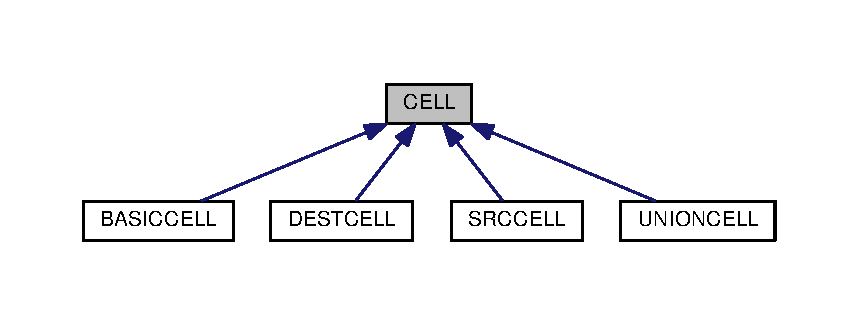
\includegraphics[width=350pt]{classCELL__inherit__graph}
\end{center}
\end{figure}


Collaboration diagram for C\+E\+L\+L\+:\nopagebreak
\begin{figure}[H]
\begin{center}
\leavevmode
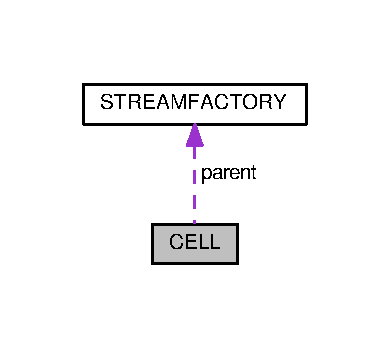
\includegraphics[width=187pt]{classCELL__coll__graph}
\end{center}
\end{figure}
\subsection*{Public Member Functions}
\begin{DoxyCompactItemize}
\item 
\hyperlink{classCELL_a266db2529e185e3f0f653f874c783c54}{C\+E\+L\+L} (\hyperlink{classPIPE}{P\+I\+P\+E} $\ast$inpipe, \hyperlink{classPIPE}{P\+I\+P\+E} $\ast$outpipe, ushort count, \hyperlink{classSTREAMFACTORY}{S\+T\+R\+E\+A\+M\+F\+A\+C\+T\+O\+R\+Y} $\ast$parent, uint X\+I\+X\+O)
\begin{DoxyCompactList}\small\item\em cell을 만드는 생성자 \end{DoxyCompactList}\item 
\hyperlink{classCELL_a8dcb65b2c6869145de9cf5056d7fe356}{C\+E\+L\+L} (\hyperlink{classPIPE}{P\+I\+P\+E} $\ast$inoutpipe, ushort count, \hyperlink{classSTREAMFACTORY}{S\+T\+R\+E\+A\+M\+F\+A\+C\+T\+O\+R\+Y} $\ast$parent, uint X\+I\+X\+O)
\begin{DoxyCompactList}\small\item\em cell을 만드는 생성자. 일반적으로 X\+I\+X\+O가 S\+O, S\+I일때 쓰인다. \end{DoxyCompactList}\item 
\hyperlink{classCELL_ae82291f0f5dd18ef2ba31e6af1a74e09}{C\+E\+L\+L} (\hyperlink{classPIPE}{P\+I\+P\+E} $\ast$inpipe, list$<$ \hyperlink{classPIPE}{P\+I\+P\+E} $\ast$ $>$ $\ast$outpipelist, ushort count, \hyperlink{classSTREAMFACTORY}{S\+T\+R\+E\+A\+M\+F\+A\+C\+T\+O\+R\+Y} $\ast$parent, uint X\+I\+X\+O)
\begin{DoxyCompactList}\small\item\em cell을 만드는 생성자. \end{DoxyCompactList}\item 
\hyperlink{classCELL_a2fad68b40d0adbecfee691618c256518}{C\+E\+L\+L} (list$<$ \hyperlink{classPIPE}{P\+I\+P\+E} $\ast$ $>$ $\ast$outpipelist, ushort count, \hyperlink{classSTREAMFACTORY}{S\+T\+R\+E\+A\+M\+F\+A\+C\+T\+O\+R\+Y} $\ast$parent, uint X\+I\+X\+O)
\begin{DoxyCompactList}\small\item\em cell을 만드는 생성자. 일반적으로 S\+O일때 쓰인다. \end{DoxyCompactList}\item 
\hyperlink{classCELL_a42a40e06fa704cbe13e1a5fbfaaaafdd}{C\+E\+L\+L} (list$<$ \hyperlink{classPIPE}{P\+I\+P\+E} $\ast$ $>$ $\ast$inpipelist, list$<$ \hyperlink{classPIPE}{P\+I\+P\+E} $\ast$ $>$ $\ast$outpipelist, ushort count, \hyperlink{classSTREAMFACTORY}{S\+T\+R\+E\+A\+M\+F\+A\+C\+T\+O\+R\+Y} $\ast$parent, uint X\+I\+X\+O)
\begin{DoxyCompactList}\small\item\em cell을 만드는 생성자. \end{DoxyCompactList}\item 
virtual void \hyperlink{classCELL_a1b048e8ac8cc57bcdff18bbcba6ed975}{make\+Worker} ()=0
\begin{DoxyCompactList}\small\item\em cell의 워커를 만드는 순수 가상 메소드 \end{DoxyCompactList}\item 
void \hyperlink{classCELL_a99661b458e7c235892c9bcd3414f1403}{scheduling\+Start} ()
\begin{DoxyCompactList}\small\item\em cell안의 워커를 스케줄링 및 실행한다. \end{DoxyCompactList}\item 
virtual void $\ast$ \hyperlink{classCELL_adcd2e66700a2c6f0cb234cbe63d2e10c}{scheduling} (void $\ast$arg)=0
\begin{DoxyCompactList}\small\item\em 실제 스케줄러의 내부 알고리즘이다. 순수 가상 메소드이다. \end{DoxyCompactList}\item 
bool \hyperlink{classCELL_a768550329a49aa05ca98f31ab859aac4}{get\+W\+O\+R\+K\+E\+R\+State} ()
\begin{DoxyCompactList}\small\item\em 워커가 하나 이상이 수행중이면 true를 반환한다. 모든 워커가 블록 되어있으면 false를 리턴한다. \end{DoxyCompactList}\item 
list$<$ \hyperlink{classPIPE}{P\+I\+P\+E} $\ast$ $>$ $\ast$ \hyperlink{classCELL_ae9f289599c3fee2e1789b81ff72742e8}{getoutpipelist} ()
\begin{DoxyCompactList}\small\item\em cell에 연결된 outpipe의 list를 반환한다. \end{DoxyCompactList}\item 
void \hyperlink{classCELL_ac9f06814e46403e615afd0a7c43d26f9}{scheduler\+Sleep} ()
\begin{DoxyCompactList}\small\item\em cell의 스케줄러를 블럭한다. \end{DoxyCompactList}\item 
void \hyperlink{classCELL_a70bb6d324838362f2feeb4ba47accc4e}{scheduler\+Wakeup} ()
\begin{DoxyCompactList}\small\item\em cell의 스케줄러를 깨운다. \end{DoxyCompactList}\item 
bool \hyperlink{classCELL_aa9a99d28684e6b16841851f4e42fcc18}{get\+C\+E\+L\+L\+State} ()
\begin{DoxyCompactList}\small\item\em cell의 스케줄러 상태를 반환한다. \end{DoxyCompactList}\item 
ushort \hyperlink{classCELL_a96407db1499c2bd1d03d23c12e7e1821}{get\+X\+I\+X\+O} ()
\begin{DoxyCompactList}\small\item\em cell의 입출력 형태를 반환한다. \end{DoxyCompactList}\end{DoxyCompactItemize}
\subsection*{Static Public Member Functions}
\begin{DoxyCompactItemize}
\item 
static void $\ast$ \hyperlink{classCELL_a9af98a9c48fa039b109f3e7bbdedf3b5}{scheduling\+\_\+wrapper} (void $\ast$context)
\begin{DoxyCompactList}\small\item\em 내부 스케줄링 알고리즘인 scheduling을 호출한다. \end{DoxyCompactList}\end{DoxyCompactItemize}
\subsection*{Protected Attributes}
\begin{DoxyCompactItemize}
\item 
\hypertarget{classCELL_a12af7a46f05c67ea5ad29d436e260897}{}list$<$ \hyperlink{classPIPE}{P\+I\+P\+E} $\ast$ $>$ $\ast$ {\bfseries inpipelist}\label{classCELL_a12af7a46f05c67ea5ad29d436e260897}

\item 
\hypertarget{classCELL_ad352add44722ccba56347f90134294bf}{}list$<$ \hyperlink{classPIPE}{P\+I\+P\+E} $\ast$ $>$ $\ast$ {\bfseries outpipelist}\label{classCELL_ad352add44722ccba56347f90134294bf}

\item 
\hypertarget{classCELL_a9daad014764db889e1eb1ae8e9a3e669}{}ushort {\bfseries count}\label{classCELL_a9daad014764db889e1eb1ae8e9a3e669}

\item 
\hypertarget{classCELL_a2134083623b7adc33f790f1bebd49193}{}\hyperlink{classSTREAMFACTORY}{S\+T\+R\+E\+A\+M\+F\+A\+C\+T\+O\+R\+Y} $\ast$ {\bfseries parent}\label{classCELL_a2134083623b7adc33f790f1bebd49193}

\item 
\hypertarget{classCELL_a5b8c354b0b11bf129bb201867e6ed1f9}{}bool {\bfseries isrun}\label{classCELL_a5b8c354b0b11bf129bb201867e6ed1f9}

\item 
\hypertarget{classCELL_a48ac64047c6cbb13258ed723df05329d}{}bool {\bfseries is\+End}\label{classCELL_a48ac64047c6cbb13258ed723df05329d}

\item 
\hypertarget{classCELL_af34bb74ac1ad036c344ba8924576e6a7}{}pthread\+\_\+t {\bfseries scheduling\+\_\+tid}\label{classCELL_af34bb74ac1ad036c344ba8924576e6a7}

\item 
\hypertarget{classCELL_abf039900f9bb3735e2d0f97d399780cd}{}list$<$ \hyperlink{classWORKER}{W\+O\+R\+K\+E\+R} $\ast$ $>$ {\bfseries workers}\label{classCELL_abf039900f9bb3735e2d0f97d399780cd}

\item 
\hypertarget{classCELL_a089446e6f9d6281652344c0f3fce062b}{}ushort {\bfseries X\+I\+X\+O}\label{classCELL_a089446e6f9d6281652344c0f3fce062b}

\item 
\hypertarget{classCELL_a97db6750f7be9deeba90eb1bf03f7bf7}{}pthread\+\_\+cond\+\_\+t {\bfseries condition}\label{classCELL_a97db6750f7be9deeba90eb1bf03f7bf7}

\item 
\hypertarget{classCELL_a85ebe512fcc57a9e7dba4318e1999cc9}{}pthread\+\_\+mutex\+\_\+t {\bfseries cond\+\_\+mutex}\label{classCELL_a85ebe512fcc57a9e7dba4318e1999cc9}

\item 
\hypertarget{classCELL_a6eb8c2b8eaff0eff3f4bf585132d73b0}{}pthread\+\_\+mutex\+\_\+t {\bfseries mutex}\label{classCELL_a6eb8c2b8eaff0eff3f4bf585132d73b0}

\end{DoxyCompactItemize}


\subsection{Detailed Description}
processing cell의 기본 구현이 들어있는 클래스 

processing cell의 기본 구현이 들어있는 클래스이다. 이 클래스는 파생되는 셀에 상속된다. \begin{DoxyAuthor}{Author}
ysmoon 
\end{DoxyAuthor}
\begin{DoxyDate}{Date}
2016-\/11-\/08 
\end{DoxyDate}
\begin{DoxyVersion}{Version}
0.\+0.\+1 
\end{DoxyVersion}


\subsection{Constructor \& Destructor Documentation}
\hypertarget{classCELL_a266db2529e185e3f0f653f874c783c54}{}\index{C\+E\+L\+L@{C\+E\+L\+L}!C\+E\+L\+L@{C\+E\+L\+L}}
\index{C\+E\+L\+L@{C\+E\+L\+L}!C\+E\+L\+L@{C\+E\+L\+L}}
\subsubsection[{C\+E\+L\+L}]{\setlength{\rightskip}{0pt plus 5cm}C\+E\+L\+L\+::\+C\+E\+L\+L (
\begin{DoxyParamCaption}
\item[{{\bf P\+I\+P\+E} $\ast$}]{inpipe, }
\item[{{\bf P\+I\+P\+E} $\ast$}]{outpipe, }
\item[{ushort}]{count, }
\item[{{\bf S\+T\+R\+E\+A\+M\+F\+A\+C\+T\+O\+R\+Y} $\ast$}]{parent, }
\item[{uint}]{X\+I\+X\+O}
\end{DoxyParamCaption}
)}\label{classCELL_a266db2529e185e3f0f653f874c783c54}


cell을 만드는 생성자 

cell을 만드는 생성자. 보통은 상속할 때 상속 생성자로 불리는 생성자이다. 
\begin{DoxyParams}{Parameters}
{\em inpipe} & cell에 대한 단일 input pipe이다. \\
\hline
{\em outpipe} & cell에 대한 단일 output pipe이다. \\
\hline
{\em count} & cell에 들어있는 worker의 개수를 정의한다. \\
\hline
{\em parent} & cell이 속한 factory를 명시한다. \\
\hline
{\em X\+I\+X\+O} & cell의 input과 output의 형태를 정의한다. S\+I\+S\+O, M\+I\+S\+O, S\+O, S\+I중 선택 \\
\hline
\end{DoxyParams}
\hypertarget{classCELL_a8dcb65b2c6869145de9cf5056d7fe356}{}\index{C\+E\+L\+L@{C\+E\+L\+L}!C\+E\+L\+L@{C\+E\+L\+L}}
\index{C\+E\+L\+L@{C\+E\+L\+L}!C\+E\+L\+L@{C\+E\+L\+L}}
\subsubsection[{C\+E\+L\+L}]{\setlength{\rightskip}{0pt plus 5cm}C\+E\+L\+L\+::\+C\+E\+L\+L (
\begin{DoxyParamCaption}
\item[{{\bf P\+I\+P\+E} $\ast$}]{inoutpipe, }
\item[{ushort}]{count, }
\item[{{\bf S\+T\+R\+E\+A\+M\+F\+A\+C\+T\+O\+R\+Y} $\ast$}]{parent, }
\item[{uint}]{X\+I\+X\+O}
\end{DoxyParamCaption}
)}\label{classCELL_a8dcb65b2c6869145de9cf5056d7fe356}


cell을 만드는 생성자. 일반적으로 X\+I\+X\+O가 S\+O, S\+I일때 쓰인다. 

cell을 만드는 생성자. 일반적으로 X\+I\+X\+O가 S\+O, S\+I일때 쓰인다. 보통은 상속할 때 상속 생성자로 불리는 생성자이다. 
\begin{DoxyParams}{Parameters}
{\em inoutpipe} & input 또는 output pipe로 쓰일 단일 파이프를 지정한다. \\
\hline
{\em count} & cell에 들어있는 worker의 개수를 정의한다. \\
\hline
{\em parent} & cell이 속한 factory를 명시한다. \\
\hline
{\em X\+I\+X\+O} & cell의 input과 output의 형태를 정의한다. S\+I\+S\+O, M\+I\+S\+O, S\+O, S\+I중 선택 \\
\hline
\end{DoxyParams}
\hypertarget{classCELL_ae82291f0f5dd18ef2ba31e6af1a74e09}{}\index{C\+E\+L\+L@{C\+E\+L\+L}!C\+E\+L\+L@{C\+E\+L\+L}}
\index{C\+E\+L\+L@{C\+E\+L\+L}!C\+E\+L\+L@{C\+E\+L\+L}}
\subsubsection[{C\+E\+L\+L}]{\setlength{\rightskip}{0pt plus 5cm}C\+E\+L\+L\+::\+C\+E\+L\+L (
\begin{DoxyParamCaption}
\item[{{\bf P\+I\+P\+E} $\ast$}]{inpipe, }
\item[{list$<$ {\bf P\+I\+P\+E} $\ast$ $>$ $\ast$}]{outpipelist, }
\item[{ushort}]{count, }
\item[{{\bf S\+T\+R\+E\+A\+M\+F\+A\+C\+T\+O\+R\+Y} $\ast$}]{parent, }
\item[{uint}]{X\+I\+X\+O}
\end{DoxyParamCaption}
)}\label{classCELL_ae82291f0f5dd18ef2ba31e6af1a74e09}


cell을 만드는 생성자. 

cell을 만드는 생성자. 보통은 상속할 때 상속 생성자로 불리는 생성자이다. 
\begin{DoxyParams}{Parameters}
{\em inpipe} & cell에 대한 단일 input pipe이다. \\
\hline
{\em outpipelist} & cell에 대한 output pipe list이다. 깊은 복사로 넘어간다. 이후 파라미터로 들어온것은 필요 없으면 메모리 해제 해야 한다. \\
\hline
{\em count} & cell에 들어있는 worker의 개수를 정의한다. \\
\hline
{\em parent} & cell이 속한 factory를 명시한다. \\
\hline
{\em X\+I\+X\+O} & cell의 input과 output의 형태를 정의한다. S\+I\+S\+O, M\+I\+S\+O, S\+O, S\+I중 선택 \\
\hline
\end{DoxyParams}
\hypertarget{classCELL_a2fad68b40d0adbecfee691618c256518}{}\index{C\+E\+L\+L@{C\+E\+L\+L}!C\+E\+L\+L@{C\+E\+L\+L}}
\index{C\+E\+L\+L@{C\+E\+L\+L}!C\+E\+L\+L@{C\+E\+L\+L}}
\subsubsection[{C\+E\+L\+L}]{\setlength{\rightskip}{0pt plus 5cm}C\+E\+L\+L\+::\+C\+E\+L\+L (
\begin{DoxyParamCaption}
\item[{list$<$ {\bf P\+I\+P\+E} $\ast$ $>$ $\ast$}]{outpipelist, }
\item[{ushort}]{count, }
\item[{{\bf S\+T\+R\+E\+A\+M\+F\+A\+C\+T\+O\+R\+Y} $\ast$}]{parent, }
\item[{uint}]{X\+I\+X\+O}
\end{DoxyParamCaption}
)}\label{classCELL_a2fad68b40d0adbecfee691618c256518}


cell을 만드는 생성자. 일반적으로 S\+O일때 쓰인다. 

cell을 만드는 생성자. 일반적으로 S\+O일때 쓰인다. 보통은 상속할 때 상속 생성자로 불리는 생성자이다. 
\begin{DoxyParams}{Parameters}
{\em outpipelist} & cell에 대한 output pipe list이다. 깊은 복사로 넘어간다. 이후 파라미터로 들어온것은 필요 없으면 메모리 해제 해야 한다. \\
\hline
{\em count} & cell에 들어있는 worker의 개수를 정의한다. \\
\hline
{\em parent} & cell이 속한 factory를 명시한다. \\
\hline
{\em X\+I\+X\+O} & cell의 input과 output의 형태를 정의한다. S\+I\+S\+O, M\+I\+S\+O, S\+O, S\+I중 선택 \\
\hline
\end{DoxyParams}
\hypertarget{classCELL_a42a40e06fa704cbe13e1a5fbfaaaafdd}{}\index{C\+E\+L\+L@{C\+E\+L\+L}!C\+E\+L\+L@{C\+E\+L\+L}}
\index{C\+E\+L\+L@{C\+E\+L\+L}!C\+E\+L\+L@{C\+E\+L\+L}}
\subsubsection[{C\+E\+L\+L}]{\setlength{\rightskip}{0pt plus 5cm}C\+E\+L\+L\+::\+C\+E\+L\+L (
\begin{DoxyParamCaption}
\item[{list$<$ {\bf P\+I\+P\+E} $\ast$ $>$ $\ast$}]{inpipelist, }
\item[{list$<$ {\bf P\+I\+P\+E} $\ast$ $>$ $\ast$}]{outpipelist, }
\item[{ushort}]{count, }
\item[{{\bf S\+T\+R\+E\+A\+M\+F\+A\+C\+T\+O\+R\+Y} $\ast$}]{parent, }
\item[{uint}]{X\+I\+X\+O}
\end{DoxyParamCaption}
)}\label{classCELL_a42a40e06fa704cbe13e1a5fbfaaaafdd}


cell을 만드는 생성자. 

cell을 만드는 생성자. 보통은 상속할 때 상속 생성자로 불리는 생성자이다. 
\begin{DoxyParams}{Parameters}
{\em inpipe} & cell에 대한 단일 input pipe list이다. 깊은 복사로 넘어간다. 이후 파라미터로 들어온것은 필요 없으면 메모리 해제 해야 한다. \\
\hline
{\em outpipelist} & cell에 대한 output pipe list이다. 깊은 복사로 넘어간다. 이후 파라미터로 들어온것은 필요 없으면 메모리 해제 해야 한다. \\
\hline
{\em count} & cell에 들어있는 worker의 개수를 정의한다. \\
\hline
{\em parent} & cell이 속한 factory를 명시한다. \\
\hline
{\em X\+I\+X\+O} & cell의 input과 output의 형태를 정의한다. S\+I\+S\+O, M\+I\+S\+O, S\+O, S\+I중 선택 \\
\hline
\end{DoxyParams}


\subsection{Member Function Documentation}
\hypertarget{classCELL_aa9a99d28684e6b16841851f4e42fcc18}{}\index{C\+E\+L\+L@{C\+E\+L\+L}!get\+C\+E\+L\+L\+State@{get\+C\+E\+L\+L\+State}}
\index{get\+C\+E\+L\+L\+State@{get\+C\+E\+L\+L\+State}!C\+E\+L\+L@{C\+E\+L\+L}}
\subsubsection[{get\+C\+E\+L\+L\+State}]{\setlength{\rightskip}{0pt plus 5cm}bool C\+E\+L\+L\+::get\+C\+E\+L\+L\+State (
\begin{DoxyParamCaption}
{}
\end{DoxyParamCaption}
)}\label{classCELL_aa9a99d28684e6b16841851f4e42fcc18}


cell의 스케줄러 상태를 반환한다. 

cell의 스케줄러 상태를 반환한다. cell의 상태는 워커 상태와 다르며 cell의 스케줄러 상태가 러닝 상태이면 true, 블럭 상태면 false를 반환한다. \begin{DoxyReturn}{Returns}
bool 
\end{DoxyReturn}
\hypertarget{classCELL_ae9f289599c3fee2e1789b81ff72742e8}{}\index{C\+E\+L\+L@{C\+E\+L\+L}!getoutpipelist@{getoutpipelist}}
\index{getoutpipelist@{getoutpipelist}!C\+E\+L\+L@{C\+E\+L\+L}}
\subsubsection[{getoutpipelist}]{\setlength{\rightskip}{0pt plus 5cm}list$<$ {\bf P\+I\+P\+E} $\ast$ $>$ $\ast$ C\+E\+L\+L\+::getoutpipelist (
\begin{DoxyParamCaption}
{}
\end{DoxyParamCaption}
)}\label{classCELL_ae9f289599c3fee2e1789b81ff72742e8}


cell에 연결된 outpipe의 list를 반환한다. 

cell에 연결된 outpipe의 list를 반환한다. \begin{DoxyReturn}{Returns}
list$<$\+P\+I\+P\+E$\ast$$>$$\ast$ 리스트 포인터를 반환한다. 
\end{DoxyReturn}
\hypertarget{classCELL_a768550329a49aa05ca98f31ab859aac4}{}\index{C\+E\+L\+L@{C\+E\+L\+L}!get\+W\+O\+R\+K\+E\+R\+State@{get\+W\+O\+R\+K\+E\+R\+State}}
\index{get\+W\+O\+R\+K\+E\+R\+State@{get\+W\+O\+R\+K\+E\+R\+State}!C\+E\+L\+L@{C\+E\+L\+L}}
\subsubsection[{get\+W\+O\+R\+K\+E\+R\+State}]{\setlength{\rightskip}{0pt plus 5cm}bool C\+E\+L\+L\+::get\+W\+O\+R\+K\+E\+R\+State (
\begin{DoxyParamCaption}
{}
\end{DoxyParamCaption}
)}\label{classCELL_a768550329a49aa05ca98f31ab859aac4}


워커가 하나 이상이 수행중이면 true를 반환한다. 모든 워커가 블록 되어있으면 false를 리턴한다. 

워커가 하나 이상이 수행중이면 true를 반환한다. 모든 워커가 블록 되어있으면 false를 리턴한다. \begin{DoxyReturn}{Returns}
bool 
\end{DoxyReturn}
\hypertarget{classCELL_a96407db1499c2bd1d03d23c12e7e1821}{}\index{C\+E\+L\+L@{C\+E\+L\+L}!get\+X\+I\+X\+O@{get\+X\+I\+X\+O}}
\index{get\+X\+I\+X\+O@{get\+X\+I\+X\+O}!C\+E\+L\+L@{C\+E\+L\+L}}
\subsubsection[{get\+X\+I\+X\+O}]{\setlength{\rightskip}{0pt plus 5cm}ushort C\+E\+L\+L\+::get\+X\+I\+X\+O (
\begin{DoxyParamCaption}
{}
\end{DoxyParamCaption}
)}\label{classCELL_a96407db1499c2bd1d03d23c12e7e1821}


cell의 입출력 형태를 반환한다. 

cell의 입출력 형태를 반환한다. S\+I\+S\+O, M\+I\+S\+O, S\+I 그리고 S\+O중 하나를 리턴한다. \begin{DoxyReturn}{Returns}
ushort S\+I\+S\+O(0) M\+I\+S\+O(1) S\+O(2) S\+I(3)을 리턴한다. 
\end{DoxyReturn}
\hypertarget{classCELL_a1b048e8ac8cc57bcdff18bbcba6ed975}{}\index{C\+E\+L\+L@{C\+E\+L\+L}!make\+Worker@{make\+Worker}}
\index{make\+Worker@{make\+Worker}!C\+E\+L\+L@{C\+E\+L\+L}}
\subsubsection[{make\+Worker}]{\setlength{\rightskip}{0pt plus 5cm}virtual void C\+E\+L\+L\+::make\+Worker (
\begin{DoxyParamCaption}
{}
\end{DoxyParamCaption}
)\hspace{0.3cm}{\ttfamily [pure virtual]}}\label{classCELL_a1b048e8ac8cc57bcdff18bbcba6ed975}


cell의 워커를 만드는 순수 가상 메소드 

실제 워커를 쓰레드화 시킨다. 사용자 지정 함수도 여기에서 할당된다. 순수 가상 메소드이므로 상속하면 구현이 필수적이다. \begin{DoxyReturn}{Returns}
void 
\end{DoxyReturn}


Implemented in \hyperlink{classBASICCELL_aacb2fd7565d13f80e407854e0a978d73}{B\+A\+S\+I\+C\+C\+E\+L\+L}, \hyperlink{classSRCCELL_a08f5dfcdead7c32e0de8967b8058f879}{S\+R\+C\+C\+E\+L\+L}, \hyperlink{classUNIONCELL_ac57cb2a3f83bf219133a9d942c24f5aa}{U\+N\+I\+O\+N\+C\+E\+L\+L}, and \hyperlink{classDESTCELL_a98ba282e719612c8dbeaca6037968a6b}{D\+E\+S\+T\+C\+E\+L\+L}.

\hypertarget{classCELL_ac9f06814e46403e615afd0a7c43d26f9}{}\index{C\+E\+L\+L@{C\+E\+L\+L}!scheduler\+Sleep@{scheduler\+Sleep}}
\index{scheduler\+Sleep@{scheduler\+Sleep}!C\+E\+L\+L@{C\+E\+L\+L}}
\subsubsection[{scheduler\+Sleep}]{\setlength{\rightskip}{0pt plus 5cm}void C\+E\+L\+L\+::scheduler\+Sleep (
\begin{DoxyParamCaption}
{}
\end{DoxyParamCaption}
)}\label{classCELL_ac9f06814e46403e615afd0a7c43d26f9}


cell의 스케줄러를 블럭한다. 

cell의 스케줄러를 블럭한다. 동작 즉시 워커가 블럭되지는 않는다. 즉, 스케줄러 블럭 후 워커가 일을 마치면 차례대로 블럭된다. cell의 state를 false로 변환시킨다. \begin{DoxyReturn}{Returns}
void 
\end{DoxyReturn}
\hypertarget{classCELL_a70bb6d324838362f2feeb4ba47accc4e}{}\index{C\+E\+L\+L@{C\+E\+L\+L}!scheduler\+Wakeup@{scheduler\+Wakeup}}
\index{scheduler\+Wakeup@{scheduler\+Wakeup}!C\+E\+L\+L@{C\+E\+L\+L}}
\subsubsection[{scheduler\+Wakeup}]{\setlength{\rightskip}{0pt plus 5cm}void C\+E\+L\+L\+::scheduler\+Wakeup (
\begin{DoxyParamCaption}
{}
\end{DoxyParamCaption}
)}\label{classCELL_a70bb6d324838362f2feeb4ba47accc4e}


cell의 스케줄러를 깨운다. 

cell의 스케줄러를 깨운다. 스케줄러를 깨우면 다시 스케줄러라 input pipe를 풀링한다. \begin{DoxyReturn}{Returns}
void 
\end{DoxyReturn}
\hypertarget{classCELL_adcd2e66700a2c6f0cb234cbe63d2e10c}{}\index{C\+E\+L\+L@{C\+E\+L\+L}!scheduling@{scheduling}}
\index{scheduling@{scheduling}!C\+E\+L\+L@{C\+E\+L\+L}}
\subsubsection[{scheduling}]{\setlength{\rightskip}{0pt plus 5cm}virtual void$\ast$ C\+E\+L\+L\+::scheduling (
\begin{DoxyParamCaption}
\item[{void $\ast$}]{arg}
\end{DoxyParamCaption}
)\hspace{0.3cm}{\ttfamily [pure virtual]}}\label{classCELL_adcd2e66700a2c6f0cb234cbe63d2e10c}


실제 스케줄러의 내부 알고리즘이다. 순수 가상 메소드이다. 

실제 스케줄러의 내부 알고리즘이다. 순수 가상 메소드이다. 즉, 파생 셀마다 스케줄링 내부 알고리즘이 달라질 수 있으므로 상속 대상자에서 함수를 정의해야 한다. 
\begin{DoxyParams}{Parameters}
{\em arg} & cell의 this 포인터이다. 즉, 상속클래스로 포인터 캐스팅하여 이용할 수 있다. 하지만 현재까지 이용하는 경우 없음 \\
\hline
\end{DoxyParams}
\begin{DoxyReturn}{Returns}
void$\ast$ 실제로는 보통 N\+U\+L\+L을 리턴하고 의미는 없다. 
\end{DoxyReturn}


Implemented in \hyperlink{classBASICCELL_a2e910313cdad1651908cca08f89be64c}{B\+A\+S\+I\+C\+C\+E\+L\+L}, \hyperlink{classSRCCELL_afa53082be31a5d956ca4fdc65b606d66}{S\+R\+C\+C\+E\+L\+L}, \hyperlink{classUNIONCELL_a0179dad91d30e7bca318bb7e3b4a4995}{U\+N\+I\+O\+N\+C\+E\+L\+L}, and \hyperlink{classDESTCELL_a19366e1b07246beeff944f5c0c3ca520}{D\+E\+S\+T\+C\+E\+L\+L}.

\hypertarget{classCELL_a9af98a9c48fa039b109f3e7bbdedf3b5}{}\index{C\+E\+L\+L@{C\+E\+L\+L}!scheduling\+\_\+wrapper@{scheduling\+\_\+wrapper}}
\index{scheduling\+\_\+wrapper@{scheduling\+\_\+wrapper}!C\+E\+L\+L@{C\+E\+L\+L}}
\subsubsection[{scheduling\+\_\+wrapper}]{\setlength{\rightskip}{0pt plus 5cm}void $\ast$ C\+E\+L\+L\+::scheduling\+\_\+wrapper (
\begin{DoxyParamCaption}
\item[{void $\ast$}]{context}
\end{DoxyParamCaption}
)\hspace{0.3cm}{\ttfamily [static]}}\label{classCELL_a9af98a9c48fa039b109f3e7bbdedf3b5}


내부 스케줄링 알고리즘인 scheduling을 호출한다. 

내부 스케줄링 알고리즘인 scheduling을 호출한다. 이 래퍼의 존재 의의는 this pointer를 넘겨주기 위함이다. 
\begin{DoxyParams}{Parameters}
{\em context} & cell의 this 포인터이다. \\
\hline
\end{DoxyParams}
\begin{DoxyReturn}{Returns}
void$\ast$ 실제로는 보통 N\+U\+L\+L을 리턴하고 의미는 없다. 
\end{DoxyReturn}
\hypertarget{classCELL_a99661b458e7c235892c9bcd3414f1403}{}\index{C\+E\+L\+L@{C\+E\+L\+L}!scheduling\+Start@{scheduling\+Start}}
\index{scheduling\+Start@{scheduling\+Start}!C\+E\+L\+L@{C\+E\+L\+L}}
\subsubsection[{scheduling\+Start}]{\setlength{\rightskip}{0pt plus 5cm}void C\+E\+L\+L\+::scheduling\+Start (
\begin{DoxyParamCaption}
{}
\end{DoxyParamCaption}
)}\label{classCELL_a99661b458e7c235892c9bcd3414f1403}


cell안의 워커를 스케줄링 및 실행한다. 

cell안의 워커를 스케줄링 및 실행한다. 내부에서 쓰레드를 만들어 최종적으로 scheduling 함수를 호출한다. scheduling\+Start -\/$>$ scheduling\+\_\+wrapper -\/$>$ scheduling 순으로 작동한다. \begin{DoxyReturn}{Returns}
void 
\end{DoxyReturn}


The documentation for this class was generated from the following files\+:\begin{DoxyCompactItemize}
\item 
include/\hyperlink{CELL_8h}{C\+E\+L\+L.\+h}\item 
C\+E\+L\+L.\+cpp\end{DoxyCompactItemize}

\hypertarget{structCLIENT}{}\section{C\+L\+I\+E\+N\+T Struct Reference}
\label{structCLIENT}\index{C\+L\+I\+E\+N\+T@{C\+L\+I\+E\+N\+T}}
\subsection*{Public Attributes}
\begin{DoxyCompactItemize}
\item 
\hypertarget{structCLIENT_a4f168b37dad1643f1fb622e3c72a6ec4}{}int {\bfseries fd}\label{structCLIENT_a4f168b37dad1643f1fb622e3c72a6ec4}

\item 
\hypertarget{structCLIENT_ae249309659a68fe4fb81404cf39a39bc}{}struct sockaddr $\ast$ {\bfseries var\+\_\+sockaddr}\label{structCLIENT_ae249309659a68fe4fb81404cf39a39bc}

\end{DoxyCompactItemize}


The documentation for this struct was generated from the following file\+:\begin{DoxyCompactItemize}
\item 
include/Type.\+h\end{DoxyCompactItemize}

\hypertarget{structCONNDATA}{}\section{C\+O\+N\+N\+D\+A\+T\+A Struct Reference}
\label{structCONNDATA}\index{C\+O\+N\+N\+D\+A\+T\+A@{C\+O\+N\+N\+D\+A\+T\+A}}
\subsection*{Public Attributes}
\begin{DoxyCompactItemize}
\item 
\hypertarget{structCONNDATA_acb00342a3e9e6c5c258f459025eccfe3}{}list$<$ \hyperlink{classPIPE}{P\+I\+P\+E} $\ast$ $>$ $\ast$ {\bfseries inpipelist}\label{structCONNDATA_acb00342a3e9e6c5c258f459025eccfe3}

\item 
\hypertarget{structCONNDATA_ad69f26f865bba9003884e7676483f14c}{}list$<$ \hyperlink{classPIPE}{P\+I\+P\+E} $\ast$ $>$ $\ast$ {\bfseries outpipelist}\label{structCONNDATA_ad69f26f865bba9003884e7676483f14c}

\item 
\hypertarget{structCONNDATA_a54fe88a540fdc7d88b611c89486b5d49}{}int {\bfseries fd}\label{structCONNDATA_a54fe88a540fdc7d88b611c89486b5d49}

\item 
\hypertarget{structCONNDATA_a0464b9e50f672664894e5f02bbd286ab}{}void $\ast$ {\bfseries thispointer}\label{structCONNDATA_a0464b9e50f672664894e5f02bbd286ab}

\end{DoxyCompactItemize}


The documentation for this struct was generated from the following file\+:\begin{DoxyCompactItemize}
\item 
include/Type.\+h\end{DoxyCompactItemize}

\hypertarget{classCONNECTION}{}\section{C\+O\+N\+N\+E\+C\+T\+I\+O\+N Class Reference}
\label{classCONNECTION}\index{C\+O\+N\+N\+E\+C\+T\+I\+O\+N@{C\+O\+N\+N\+E\+C\+T\+I\+O\+N}}
\subsection*{Public Member Functions}
\begin{DoxyCompactItemize}
\item 
\hypertarget{classCONNECTION_a5125726f68f007997156b67a9617b5cf}{}{\bfseries C\+O\+N\+N\+E\+C\+T\+I\+O\+N} (int recvport, \hyperlink{classSTREAMFACTORY}{S\+T\+R\+E\+A\+M\+F\+A\+C\+T\+O\+R\+Y} $\ast$factory)\label{classCONNECTION_a5125726f68f007997156b67a9617b5cf}

\item 
\hypertarget{classCONNECTION_a7ff7ccbd788bd5f7a47ba99530abf3e0}{}void $\ast$ {\bfseries server\+Start\+\_\+internal} (void $\ast$arg)\label{classCONNECTION_a7ff7ccbd788bd5f7a47ba99530abf3e0}

\item 
\hypertarget{classCONNECTION_af2740d50366fca10381c135a09785dd8}{}pthread\+\_\+t {\bfseries server\+Start} (\hyperlink{classPIPE}{P\+I\+P\+E} $\ast$inpipe, list$<$ \hyperlink{classPIPE}{P\+I\+P\+E} $\ast$ $>$ $\ast$outpipelist)\label{classCONNECTION_af2740d50366fca10381c135a09785dd8}

\item 
\hypertarget{classCONNECTION_a43239ade276d44c0a626fe8c4df37a61}{}void $\ast$ {\bfseries get\+\_\+in\+\_\+addr} (struct sockaddr $\ast$sa)\label{classCONNECTION_a43239ade276d44c0a626fe8c4df37a61}

\item 
\hypertarget{classCONNECTION_ab3a8e718ce95d1df393ab7a0ceca0c94}{}void $\ast$ {\bfseries sender} (void $\ast$arg)\label{classCONNECTION_ab3a8e718ce95d1df393ab7a0ceca0c94}

\item 
\hypertarget{classCONNECTION_ab164678ba891b7e205027561677fff52}{}void $\ast$ {\bfseries receiver} (void $\ast$arg)\label{classCONNECTION_ab164678ba891b7e205027561677fff52}

\item 
\hypertarget{classCONNECTION_af515385d3584b6ff051a1c6d33493509}{}void $\ast$ {\bfseries dispatcher} (void $\ast$arg)\label{classCONNECTION_af515385d3584b6ff051a1c6d33493509}

\item 
\hypertarget{classCONNECTION_ac059a7c53e9f22954b9b2060bb739d25}{}void {\bfseries setsender\+\_\+tid} (pthread\+\_\+t tid)\label{classCONNECTION_ac059a7c53e9f22954b9b2060bb739d25}

\item 
\hypertarget{classCONNECTION_a9310770dd036dfcaf531e49cad2a91f3}{}void {\bfseries setdispatcher\+\_\+tid} (pthread\+\_\+t tid)\label{classCONNECTION_a9310770dd036dfcaf531e49cad2a91f3}

\item 
\hypertarget{classCONNECTION_a5858f6269133a43b5dbe7221a78d3d22}{}bool {\bfseries get\+Conn\+State} ()\label{classCONNECTION_a5858f6269133a43b5dbe7221a78d3d22}

\item 
\hypertarget{classCONNECTION_a58b9e421d09110d58a8ee97a0d55378c}{}void {\bfseries sleep\+C\+O\+N\+N\+E\+C\+T\+O\+R} ()\label{classCONNECTION_a58b9e421d09110d58a8ee97a0d55378c}

\item 
\hypertarget{classCONNECTION_a42daf1a6d7e4ae33ed142c077eaf173b}{}void {\bfseries wakeup\+C\+O\+N\+N\+E\+C\+T\+O\+R} ()\label{classCONNECTION_a42daf1a6d7e4ae33ed142c077eaf173b}

\item 
\hypertarget{classCONNECTION_a5820c737079b8699ba43999f45e0f839}{}void {\bfseries assemble\+Packet} (char $\ast$input, uint insize, deque$<$ \hyperlink{classPACKET}{P\+A\+C\+K\+E\+T} $\ast$ $>$ $\ast$packetque, unsigned char $\ast$seq)\label{classCONNECTION_a5820c737079b8699ba43999f45e0f839}

\item 
\hypertarget{classCONNECTION_ad0ba06a5c12ec91ea98b36ad8e5f4979}{}char $\ast$ {\bfseries getassembled\+Packet} (uint $\ast$outsize, deque$<$ \hyperlink{classPACKET}{P\+A\+C\+K\+E\+T} $\ast$ $>$ $\ast$packetque)\label{classCONNECTION_ad0ba06a5c12ec91ea98b36ad8e5f4979}

\item 
\hypertarget{classCONNECTION_abdbd118327c75dca6de3f672671a5f52}{}void {\bfseries register\+\_\+user} (int fd, sockaddr $\ast$client\+\_\+addr)\label{classCONNECTION_abdbd118327c75dca6de3f672671a5f52}

\item 
\hypertarget{classCONNECTION_a4af528016616b4361943b3a086fdf62f}{}unsigned int {\bfseries getipbyfd} (int fd)\label{classCONNECTION_a4af528016616b4361943b3a086fdf62f}

\item 
\hypertarget{classCONNECTION_aa13a749c05b958d46273487de71f4c8e}{}unsigned int {\bfseries getfdbyip} (int ip)\label{classCONNECTION_aa13a749c05b958d46273487de71f4c8e}

\end{DoxyCompactItemize}
\subsection*{Static Public Member Functions}
\begin{DoxyCompactItemize}
\item 
\hypertarget{classCONNECTION_a539285f4c0510d43c6e62346c71fdf44}{}static void $\ast$ {\bfseries server\+Start\+\_\+wrapper} (void $\ast$context)\label{classCONNECTION_a539285f4c0510d43c6e62346c71fdf44}

\item 
\hypertarget{classCONNECTION_a00c2ac9ec4f67ab68ea2c3cae144456e}{}static void $\ast$ {\bfseries sender\+\_\+wrapper} (void $\ast$context)\label{classCONNECTION_a00c2ac9ec4f67ab68ea2c3cae144456e}

\item 
\hypertarget{classCONNECTION_a11682523fefd227c06ff2a9b87f156cd}{}static void $\ast$ {\bfseries receiver\+\_\+wrapper} (void $\ast$context)\label{classCONNECTION_a11682523fefd227c06ff2a9b87f156cd}

\item 
\hypertarget{classCONNECTION_a6ef84a111db27456fa1b6390f5c5e5f0}{}static void $\ast$ {\bfseries dispatcher\+\_\+wrapper} (void $\ast$context)\label{classCONNECTION_a6ef84a111db27456fa1b6390f5c5e5f0}

\end{DoxyCompactItemize}


The documentation for this class was generated from the following files\+:\begin{DoxyCompactItemize}
\item 
srcbackup/C\+O\+N\+N\+E\+C\+T\+I\+O\+N.\+h\item 
srcbackup/C\+O\+N\+N\+E\+C\+T\+I\+O\+N.\+cpp\end{DoxyCompactItemize}

\hypertarget{classDESTCELL}{}\section{D\+E\+S\+T\+C\+E\+L\+L Class Reference}
\label{classDESTCELL}\index{D\+E\+S\+T\+C\+E\+L\+L@{D\+E\+S\+T\+C\+E\+L\+L}}


destcell을 정의해놓은 클래스. factory에서 나가는 데이터의 종말 지점이다.  




{\ttfamily \#include $<$D\+E\+S\+T\+C\+E\+L\+L.\+h$>$}



Inheritance diagram for D\+E\+S\+T\+C\+E\+L\+L\+:\nopagebreak
\begin{figure}[H]
\begin{center}
\leavevmode
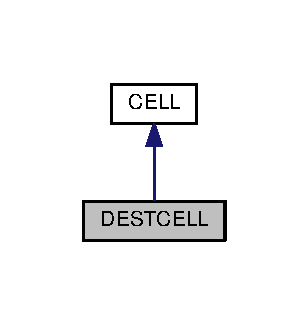
\includegraphics[width=148pt]{classDESTCELL__inherit__graph}
\end{center}
\end{figure}


Collaboration diagram for D\+E\+S\+T\+C\+E\+L\+L\+:\nopagebreak
\begin{figure}[H]
\begin{center}
\leavevmode
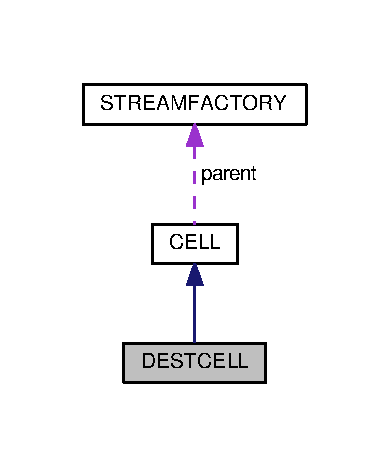
\includegraphics[width=187pt]{classDESTCELL__coll__graph}
\end{center}
\end{figure}
\subsection*{Public Member Functions}
\begin{DoxyCompactItemize}
\item 
\hyperlink{classDESTCELL_ac00a818070523ebc47f8ed37a5f5e052}{D\+E\+S\+T\+C\+E\+L\+L} (\hyperlink{classPIPE}{P\+I\+P\+E} $\ast$inpipe, \hyperlink{classSTREAMFACTORY}{S\+T\+R\+E\+A\+M\+F\+A\+C\+T\+O\+R\+Y} $\ast$parent)
\begin{DoxyCompactList}\small\item\em destcell을 만드는 생성자. \end{DoxyCompactList}\item 
\hyperlink{classDESTCELL_a17a692f1fdb71d88276696a6935032dd}{D\+E\+S\+T\+C\+E\+L\+L} (list$<$ \hyperlink{classPIPE}{P\+I\+P\+E} $\ast$ $>$ $\ast$inpipelist, \hyperlink{classSTREAMFACTORY}{S\+T\+R\+E\+A\+M\+F\+A\+C\+T\+O\+R\+Y} $\ast$parent)
\begin{DoxyCompactList}\small\item\em destcell을 만드는 생성자. \end{DoxyCompactList}\item 
virtual void \hyperlink{classDESTCELL_a98ba282e719612c8dbeaca6037968a6b}{make\+Worker} ()
\begin{DoxyCompactList}\small\item\em dummy \end{DoxyCompactList}\item 
virtual void $\ast$ \hyperlink{classDESTCELL_a19366e1b07246beeff944f5c0c3ca520}{scheduling} (void $\ast$arg)
\begin{DoxyCompactList}\small\item\em scheduling이지만, worker가 내부적으로 1개이므로 worker의 역할을 할 수 있도록 쓰레드를 생성한다. \end{DoxyCompactList}\item 
void $\ast$ \hyperlink{classDESTCELL_aa0a87ac0f210e28a81eda557b86b16d3}{D\+E\+S\+Tbroker\+\_\+start\+\_\+internal} (void $\ast$context)
\begin{DoxyCompactList}\small\item\em 센더 래퍼함수에서 실제로 수행되는 로직이 담긴 함수이다. \end{DoxyCompactList}\end{DoxyCompactItemize}
\subsection*{Static Public Member Functions}
\begin{DoxyCompactItemize}
\item 
static void $\ast$ \hyperlink{classDESTCELL_a478210dc9fb7c6fc1da37a153772464d}{D\+E\+S\+Tbroker\+\_\+start\+\_\+wrapper} (void $\ast$context)
\begin{DoxyCompactList}\small\item\em 센더 스레드를 만들기 위한 래퍼 함수이다. \end{DoxyCompactList}\end{DoxyCompactItemize}
\subsection*{Additional Inherited Members}


\subsection{Detailed Description}
destcell을 정의해놓은 클래스. factory에서 나가는 데이터의 종말 지점이다. 

destcell을 정의해놓은 클래스. factory에서 나가는 데이터의 종말 지점이다. cell의 형태를 상속하며 S\+I의 형태를 갖는다. 현재는 종말지점은 소스셀에서 연결된 디바이스 중 하나로만 한정한다. 만약 여러개의 pipe가 input으로 연결되면 라운드 로빈으로 처리한다. 이 안에서의 워커는 개념상 1만 존재한다. \begin{DoxyAuthor}{Author}
ysmoon 
\end{DoxyAuthor}
\begin{DoxyDate}{Date}
2016-\/11-\/08 
\end{DoxyDate}
\begin{DoxyVersion}{Version}
0.\+0.\+1 
\end{DoxyVersion}
\begin{DoxyRefDesc}{Todo}
\item[\hyperlink{todo__todo000001}{Todo}]D\+B로 보내기, src cell에 연결되지 않은 device도 연결을 받아 보내기 \end{DoxyRefDesc}


\subsection{Constructor \& Destructor Documentation}
\hypertarget{classDESTCELL_ac00a818070523ebc47f8ed37a5f5e052}{}\index{D\+E\+S\+T\+C\+E\+L\+L@{D\+E\+S\+T\+C\+E\+L\+L}!D\+E\+S\+T\+C\+E\+L\+L@{D\+E\+S\+T\+C\+E\+L\+L}}
\index{D\+E\+S\+T\+C\+E\+L\+L@{D\+E\+S\+T\+C\+E\+L\+L}!D\+E\+S\+T\+C\+E\+L\+L@{D\+E\+S\+T\+C\+E\+L\+L}}
\subsubsection[{D\+E\+S\+T\+C\+E\+L\+L}]{\setlength{\rightskip}{0pt plus 5cm}D\+E\+S\+T\+C\+E\+L\+L\+::\+D\+E\+S\+T\+C\+E\+L\+L (
\begin{DoxyParamCaption}
\item[{{\bf P\+I\+P\+E} $\ast$}]{inpipe, }
\item[{{\bf S\+T\+R\+E\+A\+M\+F\+A\+C\+T\+O\+R\+Y} $\ast$}]{parent}
\end{DoxyParamCaption}
)}\label{classDESTCELL_ac00a818070523ebc47f8ed37a5f5e052}


destcell을 만드는 생성자. 

destcell을 만드는 생성자. 단일 inpipe로 연결되어 있다. 
\begin{DoxyParams}{Parameters}
{\em inpipe} & destcell로 데이터를 넘겨주기 위한 pipe \\
\hline
{\em parent} & cell이 속한 factory를 명시한다. \\
\hline
\end{DoxyParams}
\hypertarget{classDESTCELL_a17a692f1fdb71d88276696a6935032dd}{}\index{D\+E\+S\+T\+C\+E\+L\+L@{D\+E\+S\+T\+C\+E\+L\+L}!D\+E\+S\+T\+C\+E\+L\+L@{D\+E\+S\+T\+C\+E\+L\+L}}
\index{D\+E\+S\+T\+C\+E\+L\+L@{D\+E\+S\+T\+C\+E\+L\+L}!D\+E\+S\+T\+C\+E\+L\+L@{D\+E\+S\+T\+C\+E\+L\+L}}
\subsubsection[{D\+E\+S\+T\+C\+E\+L\+L}]{\setlength{\rightskip}{0pt plus 5cm}D\+E\+S\+T\+C\+E\+L\+L\+::\+D\+E\+S\+T\+C\+E\+L\+L (
\begin{DoxyParamCaption}
\item[{list$<$ {\bf P\+I\+P\+E} $\ast$ $>$ $\ast$}]{inpipelist, }
\item[{{\bf S\+T\+R\+E\+A\+M\+F\+A\+C\+T\+O\+R\+Y} $\ast$}]{parent}
\end{DoxyParamCaption}
)}\label{classDESTCELL_a17a692f1fdb71d88276696a6935032dd}


destcell을 만드는 생성자. 

destcell을 만드는 생성자. 단일 inpipe로 연결되어 있다. 
\begin{DoxyParams}{Parameters}
{\em inpipelist} & destcell로 데이터를 넘겨주기 위한 pipe의 리스트. 깊은 복사를 하며 사용 이후 inpipelist가 필요가 없으면 해제하는것이 좋다. \\
\hline
{\em parent} & cell이 속한 factory를 명시한다. \\
\hline
\end{DoxyParams}


\subsection{Member Function Documentation}
\hypertarget{classDESTCELL_aa0a87ac0f210e28a81eda557b86b16d3}{}\index{D\+E\+S\+T\+C\+E\+L\+L@{D\+E\+S\+T\+C\+E\+L\+L}!D\+E\+S\+Tbroker\+\_\+start\+\_\+internal@{D\+E\+S\+Tbroker\+\_\+start\+\_\+internal}}
\index{D\+E\+S\+Tbroker\+\_\+start\+\_\+internal@{D\+E\+S\+Tbroker\+\_\+start\+\_\+internal}!D\+E\+S\+T\+C\+E\+L\+L@{D\+E\+S\+T\+C\+E\+L\+L}}
\subsubsection[{D\+E\+S\+Tbroker\+\_\+start\+\_\+internal}]{\setlength{\rightskip}{0pt plus 5cm}void $\ast$ D\+E\+S\+T\+C\+E\+L\+L\+::\+D\+E\+S\+Tbroker\+\_\+start\+\_\+internal (
\begin{DoxyParamCaption}
\item[{void $\ast$}]{context}
\end{DoxyParamCaption}
)}\label{classDESTCELL_aa0a87ac0f210e28a81eda557b86b16d3}


센더 래퍼함수에서 실제로 수행되는 로직이 담긴 함수이다. 

센더 래퍼함수에서 실제로 수행되는 로직이 담긴 함수이다. 내부에서는 input pipe들을 라운드 로빈으로 읽어 알맞는 디바이스로 데이터를 전송한다. 
\begin{DoxyParams}{Parameters}
{\em context} & (D\+E\+S\+T\+C\+E\+L\+L의) this pointer를 넘긴다. \\
\hline
\end{DoxyParams}
\begin{DoxyReturn}{Returns}
void$\ast$는 의미 없다. 
\end{DoxyReturn}
\hypertarget{classDESTCELL_a478210dc9fb7c6fc1da37a153772464d}{}\index{D\+E\+S\+T\+C\+E\+L\+L@{D\+E\+S\+T\+C\+E\+L\+L}!D\+E\+S\+Tbroker\+\_\+start\+\_\+wrapper@{D\+E\+S\+Tbroker\+\_\+start\+\_\+wrapper}}
\index{D\+E\+S\+Tbroker\+\_\+start\+\_\+wrapper@{D\+E\+S\+Tbroker\+\_\+start\+\_\+wrapper}!D\+E\+S\+T\+C\+E\+L\+L@{D\+E\+S\+T\+C\+E\+L\+L}}
\subsubsection[{D\+E\+S\+Tbroker\+\_\+start\+\_\+wrapper}]{\setlength{\rightskip}{0pt plus 5cm}void $\ast$ D\+E\+S\+T\+C\+E\+L\+L\+::\+D\+E\+S\+Tbroker\+\_\+start\+\_\+wrapper (
\begin{DoxyParamCaption}
\item[{void $\ast$}]{context}
\end{DoxyParamCaption}
)\hspace{0.3cm}{\ttfamily [static]}}\label{classDESTCELL_a478210dc9fb7c6fc1da37a153772464d}


센더 스레드를 만들기 위한 래퍼 함수이다. 

센더 스레드를 만들기 위한 래퍼 함수이다. 
\begin{DoxyParams}{Parameters}
{\em context} & (D\+E\+S\+T\+C\+E\+L\+L의) this pointer를 넘긴다. \\
\hline
\end{DoxyParams}
\begin{DoxyReturn}{Returns}
void$\ast$는 의미 없다. 
\end{DoxyReturn}
\hypertarget{classDESTCELL_a98ba282e719612c8dbeaca6037968a6b}{}\index{D\+E\+S\+T\+C\+E\+L\+L@{D\+E\+S\+T\+C\+E\+L\+L}!make\+Worker@{make\+Worker}}
\index{make\+Worker@{make\+Worker}!D\+E\+S\+T\+C\+E\+L\+L@{D\+E\+S\+T\+C\+E\+L\+L}}
\subsubsection[{make\+Worker}]{\setlength{\rightskip}{0pt plus 5cm}void D\+E\+S\+T\+C\+E\+L\+L\+::make\+Worker (
\begin{DoxyParamCaption}
{}
\end{DoxyParamCaption}
)\hspace{0.3cm}{\ttfamily [virtual]}}\label{classDESTCELL_a98ba282e719612c8dbeaca6037968a6b}


dummy 

dummy 

Implements \hyperlink{classCELL_a1b048e8ac8cc57bcdff18bbcba6ed975}{C\+E\+L\+L}.

\hypertarget{classDESTCELL_a19366e1b07246beeff944f5c0c3ca520}{}\index{D\+E\+S\+T\+C\+E\+L\+L@{D\+E\+S\+T\+C\+E\+L\+L}!scheduling@{scheduling}}
\index{scheduling@{scheduling}!D\+E\+S\+T\+C\+E\+L\+L@{D\+E\+S\+T\+C\+E\+L\+L}}
\subsubsection[{scheduling}]{\setlength{\rightskip}{0pt plus 5cm}void $\ast$ D\+E\+S\+T\+C\+E\+L\+L\+::scheduling (
\begin{DoxyParamCaption}
\item[{void $\ast$}]{arg}
\end{DoxyParamCaption}
)\hspace{0.3cm}{\ttfamily [virtual]}}\label{classDESTCELL_a19366e1b07246beeff944f5c0c3ca520}


scheduling이지만, worker가 내부적으로 1개이므로 worker의 역할을 할 수 있도록 쓰레드를 생성한다. 

scheduling이지만, worker가 내부적으로 1개이므로 worker의 역할을 할 수 있도록 쓰레드를 생성한다. 이 쓰레드에서 최종적으로 데이터를 읽고 보낸다. 
\begin{DoxyParams}{Parameters}
{\em arg} & (D\+E\+S\+T\+C\+E\+L\+L의) this pointer를 넘긴다. \\
\hline
\end{DoxyParams}
\begin{DoxyReturn}{Returns}
void$\ast$는 의미 없다. 
\end{DoxyReturn}


Implements \hyperlink{classCELL_adcd2e66700a2c6f0cb234cbe63d2e10c}{C\+E\+L\+L}.



The documentation for this class was generated from the following files\+:\begin{DoxyCompactItemize}
\item 
include/\hyperlink{DESTCELL_8h}{D\+E\+S\+T\+C\+E\+L\+L.\+h}\item 
D\+E\+S\+T\+C\+E\+L\+L.\+cpp\end{DoxyCompactItemize}

\hypertarget{classFACTORYBUILDER}{}\section{F\+A\+C\+T\+O\+R\+Y\+B\+U\+I\+L\+D\+E\+R Class Reference}
\label{classFACTORYBUILDER}\index{F\+A\+C\+T\+O\+R\+Y\+B\+U\+I\+L\+D\+E\+R@{F\+A\+C\+T\+O\+R\+Y\+B\+U\+I\+L\+D\+E\+R}}


factory builder를 만든다.  




{\ttfamily \#include $<$F\+A\+C\+T\+O\+R\+Y\+B\+U\+I\+L\+D\+E\+R.\+h$>$}

\subsection*{Public Member Functions}
\begin{DoxyCompactItemize}
\item 
void \hyperlink{classFACTORYBUILDER_a102e2a057446a1f767425b59983102df}{submit\+Scriptfor\+Factory} ()
\begin{DoxyCompactList}\small\item\em 팩토리를 만들 수 있게 스크립트를 받을 수 있는 형태가 되도록 만든다. \end{DoxyCompactList}\item 
void \hyperlink{classFACTORYBUILDER_aeb2912e73dafc162b3e0b7cdbc7fe943}{set\+M\+I\+G\+R\+A\+T\+I\+O\+N} (\hyperlink{classMIGRATION}{M\+I\+G\+R\+A\+T\+I\+O\+N} $\ast$mig)
\begin{DoxyCompactList}\small\item\em 팩토리 빌더 모듈과 마이그레이션 모듈을 연결한다. \end{DoxyCompactList}\item 
\hyperlink{classBASICCELL}{B\+A\+S\+I\+C\+C\+E\+L\+L} $\ast$ \hyperlink{classFACTORYBUILDER_ad29f6bcb828945d37bee154b247ded10}{make\+B\+A\+S\+I\+C\+C\+E\+L\+L} (int count, F\+U\+N\+C func, \hyperlink{classSTREAMFACTORY}{S\+T\+R\+E\+A\+M\+F\+A\+C\+T\+O\+R\+Y} $\ast$streamfactory)
\begin{DoxyCompactList}\small\item\em 베이직 셀 (프로세싱 셀)을 만든다. \end{DoxyCompactList}\item 
\hyperlink{classUNIONCELL}{U\+N\+I\+O\+N\+C\+E\+L\+L} $\ast$ \hyperlink{classFACTORYBUILDER_a485976fa00bdee0a822ef949c3db31e0}{make\+U\+N\+I\+O\+N\+C\+E\+L\+L} (int cellid, int count, \hyperlink{classSTREAMFACTORY}{S\+T\+R\+E\+A\+M\+F\+A\+C\+T\+O\+R\+Y} $\ast$streamfactory, int policy)
\begin{DoxyCompactList}\small\item\em 유니언 셀을 만든다. \end{DoxyCompactList}\item 
\hyperlink{classSRCCELL}{S\+R\+C\+C\+E\+L\+L} $\ast$ \hyperlink{classFACTORYBUILDER_a1378efcb11e24157cfbdb325e9cbaf2b}{make\+S\+R\+C\+C\+E\+L\+L} (int recvport, \hyperlink{classSTREAMFACTORY}{S\+T\+R\+E\+A\+M\+F\+A\+C\+T\+O\+R\+Y} $\ast$streamfactory)
\begin{DoxyCompactList}\small\item\em 데이터가 팩토리로 들어오는 소스셀을 만든다. \end{DoxyCompactList}\item 
\hyperlink{classDESTCELL}{D\+E\+S\+T\+C\+E\+L\+L} $\ast$ \hyperlink{classFACTORYBUILDER_ab56a2ef6e49fa0370c3b1138e2350d01}{make\+D\+E\+S\+T\+C\+E\+L\+L} (\hyperlink{classSTREAMFACTORY}{S\+T\+R\+E\+A\+M\+F\+A\+C\+T\+O\+R\+Y} $\ast$streamfactory)
\begin{DoxyCompactList}\small\item\em 데이터가 팩토리에서 나가는 데스티네이션셀을 만든다. \end{DoxyCompactList}\item 
void \hyperlink{classFACTORYBUILDER_ae81ea804ccbb07ef47f94c65e913d597}{linking} (\hyperlink{classCELL}{C\+E\+L\+L} $\ast$cell1, \hyperlink{classCELL}{C\+E\+L\+L} $\ast$cell2)
\begin{DoxyCompactList}\small\item\em 셀(cell1)과 셀(cell2)을 링킹한다. \end{DoxyCompactList}\item 
void \hyperlink{classFACTORYBUILDER_a47d4f78877f1fa2a6b4bc00a4c5c4471}{run\+S\+T\+R\+E\+A\+M\+F\+A\+C\+T\+O\+R\+Y} (\hyperlink{classSTREAMFACTORY}{S\+T\+R\+E\+A\+M\+F\+A\+C\+T\+O\+R\+Y} $\ast$factory)
\begin{DoxyCompactList}\small\item\em 팩토리를 가동한다. \end{DoxyCompactList}\item 
\hypertarget{classFACTORYBUILDER_a1f2abb3549a23a2fc2e25c361ad3f2fa}{}\hyperlink{classSTREAMFACTORY}{S\+T\+R\+E\+A\+M\+F\+A\+C\+T\+O\+R\+Y} $\ast$ {\bfseries create\+S\+T\+R\+E\+A\+M\+F\+A\+C\+T\+O\+R\+Y} (ushort recvport)\label{classFACTORYBUILDER_a1f2abb3549a23a2fc2e25c361ad3f2fa}

\item 
\hypertarget{classFACTORYBUILDER_a47d4f78877f1fa2a6b4bc00a4c5c4471}{}void {\bfseries run\+S\+T\+R\+E\+A\+M\+F\+A\+C\+T\+O\+R\+Y} (\hyperlink{classSTREAMFACTORY}{S\+T\+R\+E\+A\+M\+F\+A\+C\+T\+O\+R\+Y} $\ast$factory)\label{classFACTORYBUILDER_a47d4f78877f1fa2a6b4bc00a4c5c4471}

\item 
\hypertarget{classFACTORYBUILDER_a9c5c5c444ed7a2d1dc2c098793fb10a6}{}\hyperlink{classSTREAMFACTORY}{S\+T\+R\+E\+A\+M\+F\+A\+C\+T\+O\+R\+Y} $\ast$ {\bfseries get\+Stream\+Factorybyid} (int id)\label{classFACTORYBUILDER_a9c5c5c444ed7a2d1dc2c098793fb10a6}

\item 
\hypertarget{classFACTORYBUILDER_a457513572fcf3e64bee6cac741df0a3f}{}\hyperlink{classPIPE}{P\+I\+P\+E} $\ast$ {\bfseries make\+P\+I\+P\+E} (void $\ast$powner, int type, \hyperlink{classSTREAMFACTORY}{S\+T\+R\+E\+A\+M\+F\+A\+C\+T\+O\+R\+Y} $\ast$parent)\label{classFACTORYBUILDER_a457513572fcf3e64bee6cac741df0a3f}

\item 
\hypertarget{classFACTORYBUILDER_ac9de10dd42a596ef75df704e19cd2ce2}{}\hyperlink{classPIPE}{P\+I\+P\+E} $\ast$ {\bfseries find\+P\+I\+P\+E} (unsigned int id)\label{classFACTORYBUILDER_ac9de10dd42a596ef75df704e19cd2ce2}

\item 
\hypertarget{classFACTORYBUILDER_aeb2912e73dafc162b3e0b7cdbc7fe943}{}void {\bfseries set\+M\+I\+G\+R\+A\+T\+I\+O\+N} (\hyperlink{classMIGRATION}{M\+I\+G\+R\+A\+T\+I\+O\+N} $\ast$mig)\label{classFACTORYBUILDER_aeb2912e73dafc162b3e0b7cdbc7fe943}

\item 
\hypertarget{classFACTORYBUILDER_a9af3fdebefbbde78627bcb1dd11d2ede}{}\hyperlink{classMIGRATION}{M\+I\+G\+R\+A\+T\+I\+O\+N} $\ast$ {\bfseries get\+M\+I\+G\+R\+A\+T\+I\+O\+N} ()\label{classFACTORYBUILDER_a9af3fdebefbbde78627bcb1dd11d2ede}

\item 
\hypertarget{classFACTORYBUILDER_abee07310623351029b708dbd38210cc2}{}void {\bfseries start\+M\+I\+G\+R\+A\+T\+I\+O\+N} ()\label{classFACTORYBUILDER_abee07310623351029b708dbd38210cc2}

\end{DoxyCompactItemize}


\subsection{Detailed Description}
factory builder를 만든다. 

factory builder를 통해 factory를 만들 수 있다. factory builder은 전체적인 factory 관리 또한 포함한다. \begin{DoxyAuthor}{Author}
ysmoon 
\end{DoxyAuthor}
\begin{DoxyDate}{Date}
2016-\/11-\/08 
\end{DoxyDate}
\begin{DoxyVersion}{Version}
0.\+0.\+1 
\end{DoxyVersion}


\subsection{Member Function Documentation}
\hypertarget{classFACTORYBUILDER_ae81ea804ccbb07ef47f94c65e913d597}{}\index{F\+A\+C\+T\+O\+R\+Y\+B\+U\+I\+L\+D\+E\+R@{F\+A\+C\+T\+O\+R\+Y\+B\+U\+I\+L\+D\+E\+R}!linking@{linking}}
\index{linking@{linking}!F\+A\+C\+T\+O\+R\+Y\+B\+U\+I\+L\+D\+E\+R@{F\+A\+C\+T\+O\+R\+Y\+B\+U\+I\+L\+D\+E\+R}}
\subsubsection[{linking}]{\setlength{\rightskip}{0pt plus 5cm}void F\+A\+C\+T\+O\+R\+Y\+B\+U\+I\+L\+D\+E\+R\+::linking (
\begin{DoxyParamCaption}
\item[{{\bf C\+E\+L\+L} $\ast$}]{cell1, }
\item[{{\bf C\+E\+L\+L} $\ast$}]{cell2}
\end{DoxyParamCaption}
)}\label{classFACTORYBUILDER_ae81ea804ccbb07ef47f94c65e913d597}


셀(cell1)과 셀(cell2)을 링킹한다. 

실제 내부로는 셀과 셀을 링킹할 때, 파이프가 생성된다. 
\begin{DoxyParams}{Parameters}
{\em cell1} & 튜플을 출력하는 셀 \\
\hline
{\em cell2} & 튜플을 입력받는 셀 \\
\hline
\end{DoxyParams}
\hypertarget{classFACTORYBUILDER_ad29f6bcb828945d37bee154b247ded10}{}\index{F\+A\+C\+T\+O\+R\+Y\+B\+U\+I\+L\+D\+E\+R@{F\+A\+C\+T\+O\+R\+Y\+B\+U\+I\+L\+D\+E\+R}!make\+B\+A\+S\+I\+C\+C\+E\+L\+L@{make\+B\+A\+S\+I\+C\+C\+E\+L\+L}}
\index{make\+B\+A\+S\+I\+C\+C\+E\+L\+L@{make\+B\+A\+S\+I\+C\+C\+E\+L\+L}!F\+A\+C\+T\+O\+R\+Y\+B\+U\+I\+L\+D\+E\+R@{F\+A\+C\+T\+O\+R\+Y\+B\+U\+I\+L\+D\+E\+R}}
\subsubsection[{make\+B\+A\+S\+I\+C\+C\+E\+L\+L}]{\setlength{\rightskip}{0pt plus 5cm}{\bf B\+A\+S\+I\+C\+C\+E\+L\+L}$\ast$ F\+A\+C\+T\+O\+R\+Y\+B\+U\+I\+L\+D\+E\+R\+::make\+B\+A\+S\+I\+C\+C\+E\+L\+L (
\begin{DoxyParamCaption}
\item[{int}]{count, }
\item[{F\+U\+N\+C}]{func, }
\item[{{\bf S\+T\+R\+E\+A\+M\+F\+A\+C\+T\+O\+R\+Y} $\ast$}]{streamfactory}
\end{DoxyParamCaption}
)}\label{classFACTORYBUILDER_ad29f6bcb828945d37bee154b247ded10}


베이직 셀 (프로세싱 셀)을 만든다. 

베이직 셀은 기본 프로세싱 유닛을 담당하며, 입력 파이프에서 튜플을 읽어 출력 파이프로 튜플을 출력한다. 이때, 출력 파이프가 여러개라면 같은 튜플을 모든 출력파이프에 넣는다. 
\begin{DoxyParams}{Parameters}
{\em count} & 셀 내부에 생성될 워커의 개수 \\
\hline
{\em func} & T\+U\+P\+L\+E$\ast$ ($\ast$\+C\+O\+D\+E)(T\+U\+P\+L\+E$\ast$) 형태의 튜플을 처리할 코드 세그먼트를 전달한다. \\
\hline
{\em streamfactory} & 셀을 소유 할 부모 팩토리 \\
\hline
\end{DoxyParams}
\begin{DoxyRefDesc}{Todo}
\item[\hyperlink{todo__todo000002}{Todo}]processing rate와 튜플당 처리되야 하는 deadline을 정할 수 있는 파라미터 도입 예정 \begin{DoxyReturn}{Returns}
생성된 베이직 셀의 객체 포인터 
\end{DoxyReturn}
\end{DoxyRefDesc}
\hypertarget{classFACTORYBUILDER_ab56a2ef6e49fa0370c3b1138e2350d01}{}\index{F\+A\+C\+T\+O\+R\+Y\+B\+U\+I\+L\+D\+E\+R@{F\+A\+C\+T\+O\+R\+Y\+B\+U\+I\+L\+D\+E\+R}!make\+D\+E\+S\+T\+C\+E\+L\+L@{make\+D\+E\+S\+T\+C\+E\+L\+L}}
\index{make\+D\+E\+S\+T\+C\+E\+L\+L@{make\+D\+E\+S\+T\+C\+E\+L\+L}!F\+A\+C\+T\+O\+R\+Y\+B\+U\+I\+L\+D\+E\+R@{F\+A\+C\+T\+O\+R\+Y\+B\+U\+I\+L\+D\+E\+R}}
\subsubsection[{make\+D\+E\+S\+T\+C\+E\+L\+L}]{\setlength{\rightskip}{0pt plus 5cm}{\bf D\+E\+S\+T\+C\+E\+L\+L}$\ast$ F\+A\+C\+T\+O\+R\+Y\+B\+U\+I\+L\+D\+E\+R\+::make\+D\+E\+S\+T\+C\+E\+L\+L (
\begin{DoxyParamCaption}
\item[{{\bf S\+T\+R\+E\+A\+M\+F\+A\+C\+T\+O\+R\+Y} $\ast$}]{streamfactory}
\end{DoxyParamCaption}
)}\label{classFACTORYBUILDER_ab56a2ef6e49fa0370c3b1138e2350d01}


데이터가 팩토리에서 나가는 데스티네이션셀을 만든다. 

데스티네이션 셀(이하 데스트셀)은 데이터가 팩토리 밖으로 나가는 경로이다. 현재 구현은 소스셀에서 접속된 디바이스에만 데이터를 보낼 수 있다. 
\begin{DoxyParams}{Parameters}
{\em streamfactory} & 셀을 소유 할 부모 팩토리 \\
\hline
\end{DoxyParams}
\begin{DoxyReturn}{Returns}
생성된 데스트 셀의 객체 포인터 
\end{DoxyReturn}
\begin{DoxyRefDesc}{Todo}
\item[\hyperlink{todo__todo000005}{Todo}]추후 D\+B과의 출력을 담당할 예정이다. \end{DoxyRefDesc}
\hypertarget{classFACTORYBUILDER_a1378efcb11e24157cfbdb325e9cbaf2b}{}\index{F\+A\+C\+T\+O\+R\+Y\+B\+U\+I\+L\+D\+E\+R@{F\+A\+C\+T\+O\+R\+Y\+B\+U\+I\+L\+D\+E\+R}!make\+S\+R\+C\+C\+E\+L\+L@{make\+S\+R\+C\+C\+E\+L\+L}}
\index{make\+S\+R\+C\+C\+E\+L\+L@{make\+S\+R\+C\+C\+E\+L\+L}!F\+A\+C\+T\+O\+R\+Y\+B\+U\+I\+L\+D\+E\+R@{F\+A\+C\+T\+O\+R\+Y\+B\+U\+I\+L\+D\+E\+R}}
\subsubsection[{make\+S\+R\+C\+C\+E\+L\+L}]{\setlength{\rightskip}{0pt plus 5cm}{\bf S\+R\+C\+C\+E\+L\+L}$\ast$ F\+A\+C\+T\+O\+R\+Y\+B\+U\+I\+L\+D\+E\+R\+::make\+S\+R\+C\+C\+E\+L\+L (
\begin{DoxyParamCaption}
\item[{int}]{recvport, }
\item[{{\bf S\+T\+R\+E\+A\+M\+F\+A\+C\+T\+O\+R\+Y} $\ast$}]{streamfactory}
\end{DoxyParamCaption}
)}\label{classFACTORYBUILDER_a1378efcb11e24157cfbdb325e9cbaf2b}


데이터가 팩토리로 들어오는 소스셀을 만든다. 

소스셀은 팩토리로 데이터가 유입되는 경로이다. 현재 구현은 디바이스와의 통신이 이루어 질때, 디바이스가 보낸 데이터를 받는 경로이다. 
\begin{DoxyParams}{Parameters}
{\em recvport} & 연결을 대기할 리시브 포트 \\
\hline
{\em streamfactory} & 셀을 소유 할 부모 팩토리 \\
\hline
\end{DoxyParams}
\begin{DoxyReturn}{Returns}
생성된 소스 셀의 객체 포인터 
\end{DoxyReturn}
\begin{DoxyRefDesc}{Todo}
\item[\hyperlink{todo__todo000004}{Todo}]추후 D\+B등과의 입력을 담당할 예정이다. \end{DoxyRefDesc}
\hypertarget{classFACTORYBUILDER_a485976fa00bdee0a822ef949c3db31e0}{}\index{F\+A\+C\+T\+O\+R\+Y\+B\+U\+I\+L\+D\+E\+R@{F\+A\+C\+T\+O\+R\+Y\+B\+U\+I\+L\+D\+E\+R}!make\+U\+N\+I\+O\+N\+C\+E\+L\+L@{make\+U\+N\+I\+O\+N\+C\+E\+L\+L}}
\index{make\+U\+N\+I\+O\+N\+C\+E\+L\+L@{make\+U\+N\+I\+O\+N\+C\+E\+L\+L}!F\+A\+C\+T\+O\+R\+Y\+B\+U\+I\+L\+D\+E\+R@{F\+A\+C\+T\+O\+R\+Y\+B\+U\+I\+L\+D\+E\+R}}
\subsubsection[{make\+U\+N\+I\+O\+N\+C\+E\+L\+L}]{\setlength{\rightskip}{0pt plus 5cm}{\bf U\+N\+I\+O\+N\+C\+E\+L\+L}$\ast$ F\+A\+C\+T\+O\+R\+Y\+B\+U\+I\+L\+D\+E\+R\+::make\+U\+N\+I\+O\+N\+C\+E\+L\+L (
\begin{DoxyParamCaption}
\item[{int}]{cellid, }
\item[{int}]{count, }
\item[{{\bf S\+T\+R\+E\+A\+M\+F\+A\+C\+T\+O\+R\+Y} $\ast$}]{streamfactory, }
\item[{int}]{policy}
\end{DoxyParamCaption}
)}\label{classFACTORYBUILDER_a485976fa00bdee0a822ef949c3db31e0}


유니언 셀을 만든다. 

유니언 셀은 두개 이상의 튜플을 합치는 기능을 한다. 튜플의 속성은 cellid에 해당하는 셀로부터 나온 튜플의 속성을 상속받는다. 
\begin{DoxyParams}{Parameters}
{\em cellid} & 합친 튜플의 속성을 정의할 셀 아이디 (그 셀 로부터 나온 튜플의 속성을 따라간다.) \\
\hline
{\em count} & 유니언 작업을 할 워커의 개수 \\
\hline
{\em streamfactory} & 셀을 소유 할 부모 팩토리 \\
\hline
{\em policy} & P\+O\+L\+I\+C\+Y\+\_\+\+A\+L\+L\+R\+E\+A\+D\+Y인 경우, 입력 파이프에 모두 튜플을 갖고 있어 합칠 수 있을때까지 기다린다. ~\newline
 P\+O\+L\+I\+C\+Y\+\_\+\+P\+A\+R\+T\+I\+A\+L\+R\+E\+A\+D\+Y인경우, 입력 파이프에 모든 튜플을 대기하지 않는다. 단, 일부 파이프에 합칠 튜플이 없는 경우 이전에 들어온 최신 튜플을 이용해 합친다. \\
\hline
\end{DoxyParams}
\begin{DoxyRefDesc}{Todo}
\item[\hyperlink{todo__todo000003}{Todo}]processing rate와 튜플당 처리되야 하는 deadline을 정할 수 있는 파라미터 도입 예정 \begin{DoxyReturn}{Returns}
생성된 유니언 셀의 객체 포인터 
\end{DoxyReturn}
\end{DoxyRefDesc}
\hypertarget{classFACTORYBUILDER_a47d4f78877f1fa2a6b4bc00a4c5c4471}{}\index{F\+A\+C\+T\+O\+R\+Y\+B\+U\+I\+L\+D\+E\+R@{F\+A\+C\+T\+O\+R\+Y\+B\+U\+I\+L\+D\+E\+R}!run\+S\+T\+R\+E\+A\+M\+F\+A\+C\+T\+O\+R\+Y@{run\+S\+T\+R\+E\+A\+M\+F\+A\+C\+T\+O\+R\+Y}}
\index{run\+S\+T\+R\+E\+A\+M\+F\+A\+C\+T\+O\+R\+Y@{run\+S\+T\+R\+E\+A\+M\+F\+A\+C\+T\+O\+R\+Y}!F\+A\+C\+T\+O\+R\+Y\+B\+U\+I\+L\+D\+E\+R@{F\+A\+C\+T\+O\+R\+Y\+B\+U\+I\+L\+D\+E\+R}}
\subsubsection[{run\+S\+T\+R\+E\+A\+M\+F\+A\+C\+T\+O\+R\+Y}]{\setlength{\rightskip}{0pt plus 5cm}void F\+A\+C\+T\+O\+R\+Y\+B\+U\+I\+L\+D\+E\+R\+::run\+S\+T\+R\+E\+A\+M\+F\+A\+C\+T\+O\+R\+Y (
\begin{DoxyParamCaption}
\item[{{\bf S\+T\+R\+E\+A\+M\+F\+A\+C\+T\+O\+R\+Y} $\ast$}]{factory}
\end{DoxyParamCaption}
)}\label{classFACTORYBUILDER_a47d4f78877f1fa2a6b4bc00a4c5c4471}


팩토리를 가동한다. 

팩토리 내부에 등록된 모든 셀을 가동한다. \hypertarget{classFACTORYBUILDER_aeb2912e73dafc162b3e0b7cdbc7fe943}{}\index{F\+A\+C\+T\+O\+R\+Y\+B\+U\+I\+L\+D\+E\+R@{F\+A\+C\+T\+O\+R\+Y\+B\+U\+I\+L\+D\+E\+R}!set\+M\+I\+G\+R\+A\+T\+I\+O\+N@{set\+M\+I\+G\+R\+A\+T\+I\+O\+N}}
\index{set\+M\+I\+G\+R\+A\+T\+I\+O\+N@{set\+M\+I\+G\+R\+A\+T\+I\+O\+N}!F\+A\+C\+T\+O\+R\+Y\+B\+U\+I\+L\+D\+E\+R@{F\+A\+C\+T\+O\+R\+Y\+B\+U\+I\+L\+D\+E\+R}}
\subsubsection[{set\+M\+I\+G\+R\+A\+T\+I\+O\+N}]{\setlength{\rightskip}{0pt plus 5cm}void F\+A\+C\+T\+O\+R\+Y\+B\+U\+I\+L\+D\+E\+R\+::set\+M\+I\+G\+R\+A\+T\+I\+O\+N (
\begin{DoxyParamCaption}
\item[{{\bf M\+I\+G\+R\+A\+T\+I\+O\+N} $\ast$}]{mig}
\end{DoxyParamCaption}
)}\label{classFACTORYBUILDER_aeb2912e73dafc162b3e0b7cdbc7fe943}


팩토리 빌더 모듈과 마이그레이션 모듈을 연결한다. 

마이그레이션 모듈은 팩토리빌더가 만든 모든 팩토리의 마이그레이션을 지원한다. 
\begin{DoxyParams}{Parameters}
{\em mig} & 마이그레이션 객체 포인터 \\
\hline
\end{DoxyParams}
\hypertarget{classFACTORYBUILDER_a102e2a057446a1f767425b59983102df}{}\index{F\+A\+C\+T\+O\+R\+Y\+B\+U\+I\+L\+D\+E\+R@{F\+A\+C\+T\+O\+R\+Y\+B\+U\+I\+L\+D\+E\+R}!submit\+Scriptfor\+Factory@{submit\+Scriptfor\+Factory}}
\index{submit\+Scriptfor\+Factory@{submit\+Scriptfor\+Factory}!F\+A\+C\+T\+O\+R\+Y\+B\+U\+I\+L\+D\+E\+R@{F\+A\+C\+T\+O\+R\+Y\+B\+U\+I\+L\+D\+E\+R}}
\subsubsection[{submit\+Scriptfor\+Factory}]{\setlength{\rightskip}{0pt plus 5cm}void F\+A\+C\+T\+O\+R\+Y\+B\+U\+I\+L\+D\+E\+R\+::submit\+Scriptfor\+Factory (
\begin{DoxyParamCaption}
{}
\end{DoxyParamCaption}
)}\label{classFACTORYBUILDER_a102e2a057446a1f767425b59983102df}


팩토리를 만들 수 있게 스크립트를 받을 수 있는 형태가 되도록 만든다. 

이 함수를 실행하면 스크립트를 입력 받을 수 있는 형태가 된다. 메인 스크립트 당 하나의 팩토리를 확보하고 스크립트를 통해 셀들을 설치하여 완전한 하나의 팩토리를 구성해야 한다. 

The documentation for this class was generated from the following files\+:\begin{DoxyCompactItemize}
\item 
include/\hyperlink{FACTORYBUILDER_8h}{F\+A\+C\+T\+O\+R\+Y\+B\+U\+I\+L\+D\+E\+R.\+h}\item 
F\+A\+C\+T\+O\+R\+Y\+B\+U\+I\+L\+D\+E\+R.\+cpp\end{DoxyCompactItemize}

\hypertarget{classMIGRATION}{}\section{M\+I\+G\+R\+A\+T\+I\+O\+N Class Reference}
\label{classMIGRATION}\index{M\+I\+G\+R\+A\+T\+I\+O\+N@{M\+I\+G\+R\+A\+T\+I\+O\+N}}
\subsection*{Public Member Functions}
\begin{DoxyCompactItemize}
\item 
\hypertarget{classMIGRATION_aecd77ec132b2b7b8d8504d3502524e10}{}{\bfseries M\+I\+G\+R\+A\+T\+I\+O\+N} (int port, char comm)\label{classMIGRATION_aecd77ec132b2b7b8d8504d3502524e10}

\item 
\hypertarget{classMIGRATION_a1006cf4d6cb170d17dda179445125d14}{}list$<$ \hyperlink{structSERVER}{Server} $\ast$ $>$ {\bfseries getnearserver} ()\label{classMIGRATION_a1006cf4d6cb170d17dda179445125d14}

\item 
\hypertarget{classMIGRATION_a25103492408e6f7e7c5f26627d229804}{}int {\bfseries make\+Server} (ushort port)\label{classMIGRATION_a25103492408e6f7e7c5f26627d229804}

\item 
\hypertarget{classMIGRATION_a60edaac3b8203c13cf09353c678fe669}{}int {\bfseries make\+Connection} (unsigned int ip, ushort port, bool is\+Installed)\label{classMIGRATION_a60edaac3b8203c13cf09353c678fe669}

\item 
\hypertarget{classMIGRATION_a2c4e73d67f260b7a0c39192f4ad451f5}{}void {\bfseries start\+M\+I\+G\+R\+A\+T\+I\+O\+N} (int id, \hyperlink{classSTREAMFACTORY}{S\+T\+R\+E\+A\+M\+F\+A\+C\+T\+O\+R\+Y} $\ast$factory)\label{classMIGRATION_a2c4e73d67f260b7a0c39192f4ad451f5}

\item 
\hypertarget{classMIGRATION_aad4b3940495672fde4e12c894ab955c8}{}void {\bfseries waitfor\+Migration} ()\label{classMIGRATION_aad4b3940495672fde4e12c894ab955c8}

\item 
\hypertarget{classMIGRATION_ae24b1d486e36d7e505920a1980d84e6b}{}void {\bfseries setserver\+\_\+fd} (int fd)\label{classMIGRATION_ae24b1d486e36d7e505920a1980d84e6b}

\item 
\hypertarget{classMIGRATION_a59ced836a15663d210c596be12557f2f}{}int {\bfseries getserver\+\_\+fd} ()\label{classMIGRATION_a59ced836a15663d210c596be12557f2f}

\item 
\hypertarget{classMIGRATION_a3a489b688757ce0bc03a838cc63656bf}{}void {\bfseries setport} (ushort port)\label{classMIGRATION_a3a489b688757ce0bc03a838cc63656bf}

\item 
\hypertarget{classMIGRATION_a3785c32dec8ded19719f3cc9f6ab91a0}{}void {\bfseries register\+Client} (int fd)\label{classMIGRATION_a3785c32dec8ded19719f3cc9f6ab91a0}

\item 
\hypertarget{classMIGRATION_a26c622c381c8aa0e65fe5d0a1efe2a7f}{}void {\bfseries register\+Server} (int fd)\label{classMIGRATION_a26c622c381c8aa0e65fe5d0a1efe2a7f}

\item 
\hypertarget{classMIGRATION_a3936956ccc2eb23b8ae8b76a0c379d6f}{}ushort {\bfseries getport} ()\label{classMIGRATION_a3936956ccc2eb23b8ae8b76a0c379d6f}

\item 
\hypertarget{classMIGRATION_ade09b9a70f9c38106bb524e1d2190313}{}bool {\bfseries getis\+Installed} ()\label{classMIGRATION_ade09b9a70f9c38106bb524e1d2190313}

\item 
\hypertarget{classMIGRATION_a78e931d01f12c152c963ff01a95bc1a2}{}void {\bfseries setis\+Installed} (bool sw)\label{classMIGRATION_a78e931d01f12c152c963ff01a95bc1a2}

\item 
\hypertarget{classMIGRATION_a6ab6735bee3820f4f9b7109948e776ae}{}int {\bfseries get\+Clienct\+C\+E\+C} (int n)\label{classMIGRATION_a6ab6735bee3820f4f9b7109948e776ae}

\item 
\hypertarget{classMIGRATION_a1ca05f1ed042a5bd72c7f1c9f2eacfba}{}int {\bfseries get\+Server\+C\+E\+C} (int n)\label{classMIGRATION_a1ca05f1ed042a5bd72c7f1c9f2eacfba}

\end{DoxyCompactItemize}


The documentation for this class was generated from the following files\+:\begin{DoxyCompactItemize}
\item 
include/M\+I\+G\+R\+A\+T\+I\+O\+N.\+h\item 
M\+I\+G\+R\+A\+T\+I\+O\+N.\+cpp\end{DoxyCompactItemize}

\hypertarget{classPACKET}{}\section{P\+A\+C\+K\+E\+T Class Reference}
\label{classPACKET}\index{P\+A\+C\+K\+E\+T@{P\+A\+C\+K\+E\+T}}
\subsection*{Public Member Functions}
\begin{DoxyCompactItemize}
\item 
\hypertarget{classPACKET_a85db1c47f3f84b9950163c250f5736b3}{}{\bfseries P\+A\+C\+K\+E\+T} (char $\ast$in\+\_\+array, unsigned int size, unsigned char seq)\label{classPACKET_a85db1c47f3f84b9950163c250f5736b3}

\item 
\hypertarget{classPACKET_a291b51f3c7bcade7fa3029c9d3a5efbe}{}char $\ast$ {\bfseries get\+Array} ()\label{classPACKET_a291b51f3c7bcade7fa3029c9d3a5efbe}

\item 
\hypertarget{classPACKET_ab198b52f5ff4cfd7108dbe7a2e90a8f6}{}unsigned int {\bfseries get\+Size} ()\label{classPACKET_ab198b52f5ff4cfd7108dbe7a2e90a8f6}

\item 
\hypertarget{classPACKET_a2a7cdcb17df7cf81de4f047327dfb385}{}unsigned char {\bfseries get\+Seq} ()\label{classPACKET_a2a7cdcb17df7cf81de4f047327dfb385}

\item 
\hypertarget{classPACKET_ae15559d044169fe79f0f420de8503a1f}{}void {\bfseries set\+Array} (char $\ast$arr)\label{classPACKET_ae15559d044169fe79f0f420de8503a1f}

\item 
\hypertarget{classPACKET_a037feea9c09f52f6fd4ac31faa7d0540}{}void {\bfseries set\+Size} (unsigned int size)\label{classPACKET_a037feea9c09f52f6fd4ac31faa7d0540}

\end{DoxyCompactItemize}


The documentation for this class was generated from the following files\+:\begin{DoxyCompactItemize}
\item 
include/P\+A\+C\+K\+E\+T.\+h\item 
P\+A\+C\+K\+E\+T.\+cpp\end{DoxyCompactItemize}

\hypertarget{classPIPE}{}\section{P\+I\+P\+E Class Reference}
\label{classPIPE}\index{P\+I\+P\+E@{P\+I\+P\+E}}
\subsection*{Public Member Functions}
\begin{DoxyCompactItemize}
\item 
\hypertarget{classPIPE_a8c01b0df984b8c440bbcbf65d18adfa0}{}{\bfseries P\+I\+P\+E} (lockfreeq $\ast$queue, void $\ast$owner, int type, int id, \hyperlink{classSTREAMFACTORY}{S\+T\+R\+E\+A\+M\+F\+A\+C\+T\+O\+R\+Y} $\ast$parent)\label{classPIPE_a8c01b0df984b8c440bbcbf65d18adfa0}

\item 
\hypertarget{classPIPE_aa75850c5323977b0addd8b82ded50c5c}{}lockfreeq $\ast$ {\bfseries get\+Queue} ()\label{classPIPE_aa75850c5323977b0addd8b82ded50c5c}

\item 
\hypertarget{classPIPE_afb6cf810e2f2bbf4b6d6dde612fa7e4a}{}void {\bfseries registerback\+Dependency} (void $\ast$dependency, int type)\label{classPIPE_afb6cf810e2f2bbf4b6d6dde612fa7e4a}

\item 
\hypertarget{classPIPE_aa824d974401a7eb2234fb68c347ef085}{}void {\bfseries registerforward\+Dependency} (void $\ast$dependency, int type)\label{classPIPE_aa824d974401a7eb2234fb68c347ef085}

\item 
\hypertarget{classPIPE_acdd22218d8c907b07e90c99d52fc8bad}{}bool {\bfseries send\+Queue} (int fd)\label{classPIPE_acdd22218d8c907b07e90c99d52fc8bad}

\item 
\hypertarget{classPIPE_ab60c7b12bb095d63948f61b38169d9ce}{}unsigned int {\bfseries getid} ()\label{classPIPE_ab60c7b12bb095d63948f61b38169d9ce}

\item 
\hypertarget{classPIPE_a3d569671bae10ff29646feed8b495451}{}void {\bfseries install\+\_\+comp\+\_\+signal} ()\label{classPIPE_a3d569671bae10ff29646feed8b495451}

\item 
\hypertarget{classPIPE_a6608edddd645df5a90bcd22ce1391c30}{}void {\bfseries clear\+Migration} ()\label{classPIPE_a6608edddd645df5a90bcd22ce1391c30}

\item 
\hypertarget{classPIPE_a2a9c98b1de4c40e429e7c0d3745f8995}{}void {\bfseries setnewest} (\hyperlink{classTUPLE}{T\+U\+P\+L\+E} $\ast$tuple)\label{classPIPE_a2a9c98b1de4c40e429e7c0d3745f8995}

\item 
\hypertarget{classPIPE_abc831e1e81ea1355c98e0fad399ed601}{}\hyperlink{classTUPLE}{T\+U\+P\+L\+E} $\ast$ {\bfseries getnewest} (bool copied)\label{classPIPE_abc831e1e81ea1355c98e0fad399ed601}

\item 
\hypertarget{classPIPE_a25ace21c01a91d90883bd8467984f9d5}{}void {\bfseries deletenewest} ()\label{classPIPE_a25ace21c01a91d90883bd8467984f9d5}

\end{DoxyCompactItemize}


The documentation for this class was generated from the following files\+:\begin{DoxyCompactItemize}
\item 
include/P\+I\+P\+E.\+h\item 
P\+I\+P\+E.\+cpp\end{DoxyCompactItemize}

\hypertarget{structSERVER}{}\section{S\+E\+R\+V\+E\+R Struct Reference}
\label{structSERVER}\index{S\+E\+R\+V\+E\+R@{S\+E\+R\+V\+E\+R}}
\subsection*{Public Attributes}
\begin{DoxyCompactItemize}
\item 
\hypertarget{structSERVER_a5d9fee6507eb1236d34550abfd235e4b}{}unsigned int {\bfseries ip}\label{structSERVER_a5d9fee6507eb1236d34550abfd235e4b}

\item 
\hypertarget{structSERVER_acd9b37bec0e6b1360700b49daf1f95b1}{}ushort {\bfseries port}\label{structSERVER_acd9b37bec0e6b1360700b49daf1f95b1}

\item 
\hypertarget{structSERVER_af4d87b23642332eb97d95a9888ce4d1c}{}bool {\bfseries is\+Installed}\label{structSERVER_af4d87b23642332eb97d95a9888ce4d1c}

\end{DoxyCompactItemize}


The documentation for this struct was generated from the following file\+:\begin{DoxyCompactItemize}
\item 
include/M\+I\+G\+R\+A\+T\+I\+O\+N.\+h\end{DoxyCompactItemize}

\hypertarget{classSRCCELL}{}\section{S\+R\+C\+C\+E\+L\+L Class Reference}
\label{classSRCCELL}\index{S\+R\+C\+C\+E\+L\+L@{S\+R\+C\+C\+E\+L\+L}}


srccell을 정의해놓은 클래스. factory로 들어오는 데이터의 시작 지점이다. cell의 형태를 상속하며 S\+O의 형태를 갖는다.  




{\ttfamily \#include $<$S\+R\+C\+C\+E\+L\+L.\+h$>$}



Inheritance diagram for S\+R\+C\+C\+E\+L\+L\+:\nopagebreak
\begin{figure}[H]
\begin{center}
\leavevmode
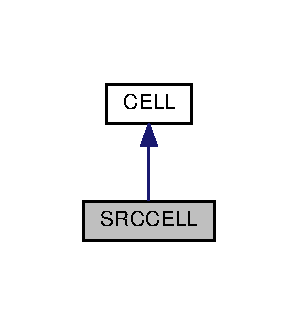
\includegraphics[width=143pt]{classSRCCELL__inherit__graph}
\end{center}
\end{figure}


Collaboration diagram for S\+R\+C\+C\+E\+L\+L\+:\nopagebreak
\begin{figure}[H]
\begin{center}
\leavevmode
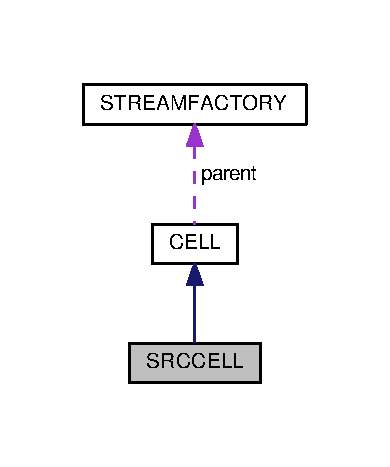
\includegraphics[width=187pt]{classSRCCELL__coll__graph}
\end{center}
\end{figure}
\subsection*{Public Member Functions}
\begin{DoxyCompactItemize}
\item 
\hyperlink{classSRCCELL_aedfd1c4aaa22c4e44ec89d2c49d67fbb}{S\+R\+C\+C\+E\+L\+L} (int recvport, \hyperlink{classPIPE}{P\+I\+P\+E} $\ast$outpipe, \hyperlink{classSTREAMFACTORY}{S\+T\+R\+E\+A\+M\+F\+A\+C\+T\+O\+R\+Y} $\ast$parent)
\begin{DoxyCompactList}\small\item\em srccell을 만드는 생성자. \end{DoxyCompactList}\item 
\hyperlink{classSRCCELL_a5c02cc02b621822b707a144aedbf5464}{S\+R\+C\+C\+E\+L\+L} (int recvport, list$<$ \hyperlink{classPIPE}{P\+I\+P\+E} $\ast$ $>$ $\ast$outpipelist, \hyperlink{classSTREAMFACTORY}{S\+T\+R\+E\+A\+M\+F\+A\+C\+T\+O\+R\+Y} $\ast$parent)
\begin{DoxyCompactList}\small\item\em srccell을 만드는 생성자. \end{DoxyCompactList}\item 
virtual void \hyperlink{classSRCCELL_a08f5dfcdead7c32e0de8967b8058f879}{make\+Worker} ()
\begin{DoxyCompactList}\small\item\em srccell의 워커(리시버)를 만들기 위해 설정한다. \end{DoxyCompactList}\item 
virtual void $\ast$ \hyperlink{classSRCCELL_afa53082be31a5d956ca4fdc65b606d66}{scheduling} (void $\ast$arg)
\begin{DoxyCompactList}\small\item\em 이름은 스케줄링이지만 리시버 브로커 쓰레드를 하나 만드는 함수이다. 브로커 쓰레드는 결국 accept를 부르며 클라이언트 연결 대기상태로 만든다. \end{DoxyCompactList}\item 
void $\ast$ \hyperlink{classSRCCELL_a895f7188ce30ab376543a63d9b40740a}{S\+R\+Cbroker\+\_\+start\+\_\+internal} (void $\ast$context)
\begin{DoxyCompactList}\small\item\em S\+R\+C\+C\+E\+L\+L에서 연결 대기를 실제로 수행하는 함수 \end{DoxyCompactList}\item 
void $\ast$ \hyperlink{classSRCCELL_acb7e9826f55fb07c8bae67889ae2d671}{S\+R\+Crecv\+\_\+start\+\_\+internal} (void $\ast$context)
\begin{DoxyCompactList}\small\item\em 실제 리시버 쓰레드에서 데이터를 받는 함수 \end{DoxyCompactList}\item 
void \hyperlink{classSRCCELL_a098c577b87319d7f5adb914e6567c7e9}{push\+Packet} (char $\ast$input, int size, deque$<$ \hyperlink{classPACKET}{P\+A\+C\+K\+E\+T} $\ast$ $>$ $\ast$packetque, unsigned char $\ast$seq)
\begin{DoxyCompactList}\small\item\em 들어온 패킷을 넣는다. \end{DoxyCompactList}\item 
char $\ast$ \hyperlink{classSRCCELL_a8e3afdc9b6c09200cd78225ded9425c0}{get\+Packetassembled} (int $\ast$size, deque$<$ \hyperlink{classPACKET}{P\+A\+C\+K\+E\+T} $\ast$ $>$ $\ast$packetque)
\begin{DoxyCompactList}\small\item\em 넣은 패킷을 하나의 처리 가능한 패킷으로 돌려 받는다. \end{DoxyCompactList}\item 
void \hyperlink{classSRCCELL_a0b41dd4b175c06ce862c4fc3d5ba10a2}{register\+Device} (\hyperlink{structCLIENT}{C\+L\+I\+E\+N\+T} $\ast$client)
\begin{DoxyCompactList}\small\item\em 디바이스와 현재 연결된 정보를 저장한다. \end{DoxyCompactList}\end{DoxyCompactItemize}
\subsection*{Static Public Member Functions}
\begin{DoxyCompactItemize}
\item 
static void $\ast$ \hyperlink{classSRCCELL_a2be96e34bed6a9186ec85772febdd50b}{S\+R\+Cbroker\+\_\+start\+\_\+wrapper} (void $\ast$context)
\begin{DoxyCompactList}\small\item\em 브로커 쓰레드에서 실제로 실행되는 래퍼 함수. \end{DoxyCompactList}\item 
static void $\ast$ \hyperlink{classSRCCELL_a7957253a55cddb0c37d3db9c39077387}{S\+R\+Crecv\+\_\+start\+\_\+wrapper} (void $\ast$context)
\begin{DoxyCompactList}\small\item\em S\+R\+C\+C\+E\+L\+L에서 대기상태에서 연결요청이 들어왔을 때 만드는 리시버 쓰레드에 들어가는 함수 \end{DoxyCompactList}\end{DoxyCompactItemize}
\subsection*{Additional Inherited Members}


\subsection{Detailed Description}
srccell을 정의해놓은 클래스. factory로 들어오는 데이터의 시작 지점이다. cell의 형태를 상속하며 S\+O의 형태를 갖는다. 

srccell을 정의해놓은 클래스. cell의 형태를 상속하며 S\+O의 형태를 갖는다. 현재는 하나의 소스셀은 서버를 만들고 여기에 디바이스가 접속할 수 있게만 되어 있다. \begin{DoxyAuthor}{Author}
ysmoon 
\end{DoxyAuthor}
\begin{DoxyDate}{Date}
2016-\/11-\/08 
\end{DoxyDate}
\begin{DoxyVersion}{Version}
0.\+0.\+1 
\end{DoxyVersion}


\subsection{Constructor \& Destructor Documentation}
\hypertarget{classSRCCELL_aedfd1c4aaa22c4e44ec89d2c49d67fbb}{}\index{S\+R\+C\+C\+E\+L\+L@{S\+R\+C\+C\+E\+L\+L}!S\+R\+C\+C\+E\+L\+L@{S\+R\+C\+C\+E\+L\+L}}
\index{S\+R\+C\+C\+E\+L\+L@{S\+R\+C\+C\+E\+L\+L}!S\+R\+C\+C\+E\+L\+L@{S\+R\+C\+C\+E\+L\+L}}
\subsubsection[{S\+R\+C\+C\+E\+L\+L}]{\setlength{\rightskip}{0pt plus 5cm}S\+R\+C\+C\+E\+L\+L\+::\+S\+R\+C\+C\+E\+L\+L (
\begin{DoxyParamCaption}
\item[{int}]{recvport, }
\item[{{\bf P\+I\+P\+E} $\ast$}]{outpipe, }
\item[{{\bf S\+T\+R\+E\+A\+M\+F\+A\+C\+T\+O\+R\+Y} $\ast$}]{parent}
\end{DoxyParamCaption}
)}\label{classSRCCELL_aedfd1c4aaa22c4e44ec89d2c49d67fbb}


srccell을 만드는 생성자. 

dsetcell을 만드는 생성자. 워커는 srccell에 연결된 디바이스당 하나가 생긴다. 스케줄링 개념은 없으며 일반적 서버-\/클라이언트 모델에 서버에서의 리시버 스레드 형태를 워커로써 갖는다. 
\begin{DoxyParams}{Parameters}
{\em recvport} & 소스셀에 접속할 때의 포트를 정의한다. \\
\hline
{\em outpipe} & cell에 대한 단일 output pipe이다. \\
\hline
{\em parent} & cell이 속한 factory를 명시한다. \\
\hline
\end{DoxyParams}
\hypertarget{classSRCCELL_a5c02cc02b621822b707a144aedbf5464}{}\index{S\+R\+C\+C\+E\+L\+L@{S\+R\+C\+C\+E\+L\+L}!S\+R\+C\+C\+E\+L\+L@{S\+R\+C\+C\+E\+L\+L}}
\index{S\+R\+C\+C\+E\+L\+L@{S\+R\+C\+C\+E\+L\+L}!S\+R\+C\+C\+E\+L\+L@{S\+R\+C\+C\+E\+L\+L}}
\subsubsection[{S\+R\+C\+C\+E\+L\+L}]{\setlength{\rightskip}{0pt plus 5cm}S\+R\+C\+C\+E\+L\+L\+::\+S\+R\+C\+C\+E\+L\+L (
\begin{DoxyParamCaption}
\item[{int}]{recvport, }
\item[{list$<$ {\bf P\+I\+P\+E} $\ast$ $>$ $\ast$}]{outpipelist, }
\item[{{\bf S\+T\+R\+E\+A\+M\+F\+A\+C\+T\+O\+R\+Y} $\ast$}]{parent}
\end{DoxyParamCaption}
)}\label{classSRCCELL_a5c02cc02b621822b707a144aedbf5464}


srccell을 만드는 생성자. 

destcell을 만드는 생성자. 워커는 srccell에 연결된 디바이스당 하나가 생긴다. 스케줄링 개념은 없으며 일반적 서버-\/클라이언트 모델에 서버에서의 리시버 스레드 형태를 워커로써 갖는다. 
\begin{DoxyParams}{Parameters}
{\em recvport} & 소스셀에 접속할 때의 포트를 정의한다. \\
\hline
{\em outpipelist} & cell에 대한 output pipe list를 넘겨준다. 포인터이며 안에서는 깊은복사가 일어난다. 파라미터로 들어온 포인터는 필요없으면 해제하는것이 좋다. \\
\hline
{\em parent} & cell이 속한 factory를 명시한다. \\
\hline
\end{DoxyParams}


\subsection{Member Function Documentation}
\hypertarget{classSRCCELL_a8e3afdc9b6c09200cd78225ded9425c0}{}\index{S\+R\+C\+C\+E\+L\+L@{S\+R\+C\+C\+E\+L\+L}!get\+Packetassembled@{get\+Packetassembled}}
\index{get\+Packetassembled@{get\+Packetassembled}!S\+R\+C\+C\+E\+L\+L@{S\+R\+C\+C\+E\+L\+L}}
\subsubsection[{get\+Packetassembled}]{\setlength{\rightskip}{0pt plus 5cm}char $\ast$ S\+R\+C\+C\+E\+L\+L\+::get\+Packetassembled (
\begin{DoxyParamCaption}
\item[{int $\ast$}]{size, }
\item[{deque$<$ {\bf P\+A\+C\+K\+E\+T} $\ast$ $>$ $\ast$}]{packetque}
\end{DoxyParamCaption}
)}\label{classSRCCELL_a8e3afdc9b6c09200cd78225ded9425c0}


넣은 패킷을 하나의 처리 가능한 패킷으로 돌려 받는다. 

넣은 패킷을 하나의 처리 가능한 패킷으로 돌려받는다. 처리 가능한 패킷이란 프로토콜을 완벽히 가지고 있고, 프로토콜만큼의 데이터 사이즈를 가진 패킷을 말한다. 
\begin{DoxyParams}{Parameters}
{\em size} & 하나의 처리 가능한 패킷의 전체 사이즈 \\
\hline
{\em packetque} & 들어온 패킷을 저장해놓은 큐 \\
\hline
\end{DoxyParams}
\hypertarget{classSRCCELL_a08f5dfcdead7c32e0de8967b8058f879}{}\index{S\+R\+C\+C\+E\+L\+L@{S\+R\+C\+C\+E\+L\+L}!make\+Worker@{make\+Worker}}
\index{make\+Worker@{make\+Worker}!S\+R\+C\+C\+E\+L\+L@{S\+R\+C\+C\+E\+L\+L}}
\subsubsection[{make\+Worker}]{\setlength{\rightskip}{0pt plus 5cm}void S\+R\+C\+C\+E\+L\+L\+::make\+Worker (
\begin{DoxyParamCaption}
{}
\end{DoxyParamCaption}
)\hspace{0.3cm}{\ttfamily [virtual]}}\label{classSRCCELL_a08f5dfcdead7c32e0de8967b8058f879}


srccell의 워커(리시버)를 만들기 위해 설정한다. 

srccell의 워커(리시버)를 만들기 위해 설정한다. \begin{DoxyReturn}{Returns}
void 의미 없음 
\end{DoxyReturn}


Implements \hyperlink{classCELL_a1b048e8ac8cc57bcdff18bbcba6ed975}{C\+E\+L\+L}.

\hypertarget{classSRCCELL_a098c577b87319d7f5adb914e6567c7e9}{}\index{S\+R\+C\+C\+E\+L\+L@{S\+R\+C\+C\+E\+L\+L}!push\+Packet@{push\+Packet}}
\index{push\+Packet@{push\+Packet}!S\+R\+C\+C\+E\+L\+L@{S\+R\+C\+C\+E\+L\+L}}
\subsubsection[{push\+Packet}]{\setlength{\rightskip}{0pt plus 5cm}void S\+R\+C\+C\+E\+L\+L\+::push\+Packet (
\begin{DoxyParamCaption}
\item[{char $\ast$}]{input, }
\item[{int}]{size, }
\item[{deque$<$ {\bf P\+A\+C\+K\+E\+T} $\ast$ $>$ $\ast$}]{packetque, }
\item[{unsigned char $\ast$}]{seq}
\end{DoxyParamCaption}
)}\label{classSRCCELL_a098c577b87319d7f5adb914e6567c7e9}


들어온 패킷을 넣는다. 

들어온 패킷을 넣는다. 이 패킷들은 get\+Packetassembled에서 조립되어 받을 수 있다. 
\begin{DoxyParams}{Parameters}
{\em input} & 패킷의 바이트 스트림 \\
\hline
{\em size} & 들어온 패킷의 사이즈 \\
\hline
{\em packetque} & 들어온 패킷을 저장해놓은 큐 \\
\hline
{\em seq} & 패킷의 시퀀스 넘버를 할당하기 위한 공유변수 \\
\hline
\end{DoxyParams}
\hypertarget{classSRCCELL_a0b41dd4b175c06ce862c4fc3d5ba10a2}{}\index{S\+R\+C\+C\+E\+L\+L@{S\+R\+C\+C\+E\+L\+L}!register\+Device@{register\+Device}}
\index{register\+Device@{register\+Device}!S\+R\+C\+C\+E\+L\+L@{S\+R\+C\+C\+E\+L\+L}}
\subsubsection[{register\+Device}]{\setlength{\rightskip}{0pt plus 5cm}void S\+R\+C\+C\+E\+L\+L\+::register\+Device (
\begin{DoxyParamCaption}
\item[{{\bf C\+L\+I\+E\+N\+T} $\ast$}]{client}
\end{DoxyParamCaption}
)}\label{classSRCCELL_a0b41dd4b175c06ce862c4fc3d5ba10a2}


디바이스와 현재 연결된 정보를 저장한다. 

디바이스와 현재 연결된 정보를 저장한다. 이 정보는 나중에 destcell에서 데이터를 보낼 때 사용된다. 
\begin{DoxyParams}{Parameters}
{\em client} & 디바이스의 접속 정보이다. 연결 시 필요한 sockaddr과 fd을 가지고 있다. \\
\hline
\end{DoxyParams}
\hypertarget{classSRCCELL_afa53082be31a5d956ca4fdc65b606d66}{}\index{S\+R\+C\+C\+E\+L\+L@{S\+R\+C\+C\+E\+L\+L}!scheduling@{scheduling}}
\index{scheduling@{scheduling}!S\+R\+C\+C\+E\+L\+L@{S\+R\+C\+C\+E\+L\+L}}
\subsubsection[{scheduling}]{\setlength{\rightskip}{0pt plus 5cm}void $\ast$ S\+R\+C\+C\+E\+L\+L\+::scheduling (
\begin{DoxyParamCaption}
\item[{void $\ast$}]{arg}
\end{DoxyParamCaption}
)\hspace{0.3cm}{\ttfamily [virtual]}}\label{classSRCCELL_afa53082be31a5d956ca4fdc65b606d66}


이름은 스케줄링이지만 리시버 브로커 쓰레드를 하나 만드는 함수이다. 브로커 쓰레드는 결국 accept를 부르며 클라이언트 연결 대기상태로 만든다. 

이름은 스케줄링이지만 리시버 브로커 쓰레드를 하나 만드는 함수이다. 브로커 쓰레드는 결국 accept를 부르며 클라이언트 연결 대기상태로 만든다. \begin{DoxyReturn}{Returns}
void 의미 없음 
\end{DoxyReturn}


Implements \hyperlink{classCELL_adcd2e66700a2c6f0cb234cbe63d2e10c}{C\+E\+L\+L}.

\hypertarget{classSRCCELL_a895f7188ce30ab376543a63d9b40740a}{}\index{S\+R\+C\+C\+E\+L\+L@{S\+R\+C\+C\+E\+L\+L}!S\+R\+Cbroker\+\_\+start\+\_\+internal@{S\+R\+Cbroker\+\_\+start\+\_\+internal}}
\index{S\+R\+Cbroker\+\_\+start\+\_\+internal@{S\+R\+Cbroker\+\_\+start\+\_\+internal}!S\+R\+C\+C\+E\+L\+L@{S\+R\+C\+C\+E\+L\+L}}
\subsubsection[{S\+R\+Cbroker\+\_\+start\+\_\+internal}]{\setlength{\rightskip}{0pt plus 5cm}void $\ast$ S\+R\+C\+C\+E\+L\+L\+::\+S\+R\+Cbroker\+\_\+start\+\_\+internal (
\begin{DoxyParamCaption}
\item[{void $\ast$}]{context}
\end{DoxyParamCaption}
)}\label{classSRCCELL_a895f7188ce30ab376543a63d9b40740a}


S\+R\+C\+C\+E\+L\+L에서 연결 대기를 실제로 수행하는 함수 

S\+R\+C\+C\+E\+L\+L에서 연결 대기를 실제로 수행하는 함수 this pointer를 이용할 수 있다. 
\begin{DoxyParams}{Parameters}
{\em context} & (S\+R\+C\+E\+L\+L의)this pointer가 들어온다. \\
\hline
\end{DoxyParams}
\begin{DoxyReturn}{Returns}
void$\ast$ 의미 없음 
\end{DoxyReturn}
\hypertarget{classSRCCELL_a2be96e34bed6a9186ec85772febdd50b}{}\index{S\+R\+C\+C\+E\+L\+L@{S\+R\+C\+C\+E\+L\+L}!S\+R\+Cbroker\+\_\+start\+\_\+wrapper@{S\+R\+Cbroker\+\_\+start\+\_\+wrapper}}
\index{S\+R\+Cbroker\+\_\+start\+\_\+wrapper@{S\+R\+Cbroker\+\_\+start\+\_\+wrapper}!S\+R\+C\+C\+E\+L\+L@{S\+R\+C\+C\+E\+L\+L}}
\subsubsection[{S\+R\+Cbroker\+\_\+start\+\_\+wrapper}]{\setlength{\rightskip}{0pt plus 5cm}void $\ast$ S\+R\+C\+C\+E\+L\+L\+::\+S\+R\+Cbroker\+\_\+start\+\_\+wrapper (
\begin{DoxyParamCaption}
\item[{void $\ast$}]{context}
\end{DoxyParamCaption}
)\hspace{0.3cm}{\ttfamily [static]}}\label{classSRCCELL_a2be96e34bed6a9186ec85772febdd50b}


브로커 쓰레드에서 실제로 실행되는 래퍼 함수. 

브로커 쓰레드에서 실제로 실행되는 래퍼 함수. 존재 의의는 this 포인터를 넘기고 사용하기 위한 trick함수이다. 
\begin{DoxyParams}{Parameters}
{\em arg} & (S\+R\+C\+E\+L\+L의)this pointer가 들어온다. \\
\hline
\end{DoxyParams}
\begin{DoxyReturn}{Returns}
void$\ast$ 의미 없음 
\end{DoxyReturn}
\hypertarget{classSRCCELL_acb7e9826f55fb07c8bae67889ae2d671}{}\index{S\+R\+C\+C\+E\+L\+L@{S\+R\+C\+C\+E\+L\+L}!S\+R\+Crecv\+\_\+start\+\_\+internal@{S\+R\+Crecv\+\_\+start\+\_\+internal}}
\index{S\+R\+Crecv\+\_\+start\+\_\+internal@{S\+R\+Crecv\+\_\+start\+\_\+internal}!S\+R\+C\+C\+E\+L\+L@{S\+R\+C\+C\+E\+L\+L}}
\subsubsection[{S\+R\+Crecv\+\_\+start\+\_\+internal}]{\setlength{\rightskip}{0pt plus 5cm}void $\ast$ S\+R\+C\+C\+E\+L\+L\+::\+S\+R\+Crecv\+\_\+start\+\_\+internal (
\begin{DoxyParamCaption}
\item[{void $\ast$}]{context}
\end{DoxyParamCaption}
)}\label{classSRCCELL_acb7e9826f55fb07c8bae67889ae2d671}


실제 리시버 쓰레드에서 데이터를 받는 함수 

실제 리시버 쓰레드에서 데이터를 받는 함수. wrapper 함수에서 부른다. 
\begin{DoxyParams}{Parameters}
{\em context} & (S\+R\+C\+E\+L\+L의)this pointer가 들어온다. \\
\hline
\end{DoxyParams}
\begin{DoxyReturn}{Returns}
void$\ast$ 의미 없음 
\end{DoxyReturn}
\hypertarget{classSRCCELL_a7957253a55cddb0c37d3db9c39077387}{}\index{S\+R\+C\+C\+E\+L\+L@{S\+R\+C\+C\+E\+L\+L}!S\+R\+Crecv\+\_\+start\+\_\+wrapper@{S\+R\+Crecv\+\_\+start\+\_\+wrapper}}
\index{S\+R\+Crecv\+\_\+start\+\_\+wrapper@{S\+R\+Crecv\+\_\+start\+\_\+wrapper}!S\+R\+C\+C\+E\+L\+L@{S\+R\+C\+C\+E\+L\+L}}
\subsubsection[{S\+R\+Crecv\+\_\+start\+\_\+wrapper}]{\setlength{\rightskip}{0pt plus 5cm}void $\ast$ S\+R\+C\+C\+E\+L\+L\+::\+S\+R\+Crecv\+\_\+start\+\_\+wrapper (
\begin{DoxyParamCaption}
\item[{void $\ast$}]{context}
\end{DoxyParamCaption}
)\hspace{0.3cm}{\ttfamily [static]}}\label{classSRCCELL_a7957253a55cddb0c37d3db9c39077387}


S\+R\+C\+C\+E\+L\+L에서 대기상태에서 연결요청이 들어왔을 때 만드는 리시버 쓰레드에 들어가는 함수 

S\+R\+C\+C\+E\+L\+L에서 대기상태에서 연결요청이 들어왔을 때 만드는 리시버 쓰레드에 들어가는 함수. 쓰레드당 디바이스가 1\+:1로 매핑되어 생성된다. 
\begin{DoxyParams}{Parameters}
{\em context} & (S\+R\+C\+E\+L\+L의)this pointer가 들어온다. \\
\hline
\end{DoxyParams}
\begin{DoxyReturn}{Returns}
void$\ast$ 의미 없음 
\end{DoxyReturn}


The documentation for this class was generated from the following files\+:\begin{DoxyCompactItemize}
\item 
include/\hyperlink{SRCCELL_8h}{S\+R\+C\+C\+E\+L\+L.\+h}\item 
S\+R\+C\+C\+E\+L\+L.\+cpp\end{DoxyCompactItemize}

\hypertarget{classSTREAMFACTORY}{}\section{S\+T\+R\+E\+A\+M\+F\+A\+C\+T\+O\+R\+Y Class Reference}
\label{classSTREAMFACTORY}\index{S\+T\+R\+E\+A\+M\+F\+A\+C\+T\+O\+R\+Y@{S\+T\+R\+E\+A\+M\+F\+A\+C\+T\+O\+R\+Y}}
\subsection*{Public Member Functions}
\begin{DoxyCompactItemize}
\item 
\hypertarget{classSTREAMFACTORY_adb6e711f4314ea889cb77d26c1d11401}{}void {\bfseries factory\+Start} ()\label{classSTREAMFACTORY_adb6e711f4314ea889cb77d26c1d11401}

\item 
\hypertarget{classSTREAMFACTORY_a048304e01d2af328ab82a4057b3f4e6e}{}list$<$ \hyperlink{classCELL}{C\+E\+L\+L} $\ast$ $>$ {\bfseries get\+C\+E\+L\+Ls} ()\label{classSTREAMFACTORY_a048304e01d2af328ab82a4057b3f4e6e}

\item 
\hypertarget{classSTREAMFACTORY_aee1d4f9e86a437a9863a344ea2c60343}{}void {\bfseries register\+C\+E\+L\+L} (\hyperlink{classCELL}{C\+E\+L\+L} $\ast$cell)\label{classSTREAMFACTORY_aee1d4f9e86a437a9863a344ea2c60343}

\item 
\hypertarget{classSTREAMFACTORY_adebc3a141db55b66ffeebc3ee36fd50d}{}bool {\bfseries get\+S\+T\+R\+E\+A\+M\+F\+A\+C\+T\+O\+R\+Y\+State} ()\label{classSTREAMFACTORY_adebc3a141db55b66ffeebc3ee36fd50d}

\item 
\hypertarget{classSTREAMFACTORY_af3c34f23b441fd0a5715a2d3e7540aaa}{}bool {\bfseries set\+S\+T\+R\+E\+A\+M\+F\+A\+C\+T\+O\+R\+Y\+State} (bool state)\label{classSTREAMFACTORY_af3c34f23b441fd0a5715a2d3e7540aaa}

\item 
\hypertarget{classSTREAMFACTORY_a20b9cfa0733b72f5f5be02b4d3e6f599}{}void {\bfseries install\+Received\+Data} (\hyperlink{classTUPLE}{T\+U\+P\+L\+E} $\ast$data)\label{classSTREAMFACTORY_a20b9cfa0733b72f5f5be02b4d3e6f599}

\item 
\hypertarget{classSTREAMFACTORY_a5e0920b25ff163b4e4c2df71a2e4f07d}{}list$<$ \hyperlink{structCLIENT}{C\+L\+I\+E\+N\+T} $\ast$ $>$ $\ast$ {\bfseries getsrcdevices} ()\label{classSTREAMFACTORY_a5e0920b25ff163b4e4c2df71a2e4f07d}

\item 
\hypertarget{classSTREAMFACTORY_ac4b55aa4e63f0fdd448b868fd8b64b09}{}\hyperlink{structCLIENT}{C\+L\+I\+E\+N\+T} $\ast$ {\bfseries get\+Clientbyip} (unsigned int ip)\label{classSTREAMFACTORY_ac4b55aa4e63f0fdd448b868fd8b64b09}

\item 
\hypertarget{classSTREAMFACTORY_ad9090e3e710248bdf02df4b12f608f95}{}\hyperlink{structCLIENT}{C\+L\+I\+E\+N\+T} $\ast$ {\bfseries get\+Clientbyfd} (unsigned int fd)\label{classSTREAMFACTORY_ad9090e3e710248bdf02df4b12f608f95}

\item 
\hypertarget{classSTREAMFACTORY_a6f8e47599501134534b0957a8c2cd6dc}{}void {\bfseries printtasks} ()\label{classSTREAMFACTORY_a6f8e47599501134534b0957a8c2cd6dc}

\end{DoxyCompactItemize}


The documentation for this class was generated from the following files\+:\begin{DoxyCompactItemize}
\item 
include/S\+T\+R\+E\+A\+M\+F\+A\+C\+T\+O\+R\+Y.\+h\item 
S\+T\+R\+E\+A\+M\+F\+A\+C\+T\+O\+R\+Y.\+cpp\end{DoxyCompactItemize}

\hypertarget{classTUPLE}{}\section{T\+U\+P\+L\+E Class Reference}
\label{classTUPLE}\index{T\+U\+P\+L\+E@{T\+U\+P\+L\+E}}


data의 교환단위인 tuple을 정의한 클래스이다.  




{\ttfamily \#include $<$T\+U\+P\+L\+E.\+h$>$}

\subsection*{Public Member Functions}
\begin{DoxyCompactItemize}
\item 
\hyperlink{classTUPLE_aed245ec6fb2cd8e94cd9bc1e7eb4a86d}{T\+U\+P\+L\+E} (char $\ast$data, ushort n\+Len, ushort seq, int fd)
\begin{DoxyCompactList}\small\item\em T\+U\+P\+L\+E을 만드는 생성자. 이 생성자는 프로토콜을 가진 raw data에서 tuple로 전환하기 위한 생성자이다. \end{DoxyCompactList}\item 
\hyperlink{classTUPLE_a00b079f9d403adb63356880c62d48e22}{T\+U\+P\+L\+E} (ushort n\+Len, int fd, int type)
\begin{DoxyCompactList}\small\item\em T\+U\+P\+L\+E을 만드는 생성자. 이 생성자는 새로운 튜플을 만들어야 할 때 쓰인다. \end{DoxyCompactList}\item 
\hyperlink{classTUPLE_ac92a492d3f8a793fe02fe364244c34af}{T\+U\+P\+L\+E} (char $\ast$packet, bool is\+Special)
\begin{DoxyCompactList}\small\item\em T\+U\+P\+L\+E을 만드는 생성자. 이 생성자는 migration에 쓰인다. (migration은 특수 프로토콜을 쓰기 때문..) \end{DoxyCompactList}\item 
bool \hyperlink{classTUPLE_a15e6fe7915b00b6fce4842630dc3bbb0}{validity} ()
\begin{DoxyCompactList}\small\item\em 튜플이 유효한 튜플인지 체크한다. \end{DoxyCompactList}\item 
uchar \hyperlink{classTUPLE_a6616af9acaa70eadc0d4110a6b81a642}{gettype} ()
\begin{DoxyCompactList}\small\item\em 튜플의 type 또는 attribute를 가져온다. \end{DoxyCompactList}\item 
char $\ast$ \hyperlink{classTUPLE_a92c2046bfd6da6f0cfee98f3eb79a16b}{getcontent} ()
\begin{DoxyCompactList}\small\item\em 튜플이 가지고 있는 프로토콜을 제외한 byte array의 포인터를 받아온다. \end{DoxyCompactList}\item 
char $\ast$ \hyperlink{classTUPLE_aee1504a1fcdc572c7882a3a2bfdb68c1}{getdata} ()
\begin{DoxyCompactList}\small\item\em 튜플이 가지고 있는 프로토콜을 포함한 byte array의 포인터를 받아온다. \end{DoxyCompactList}\item 
ushort \hyperlink{classTUPLE_ab76925f0b573319312d68b99b01c430b}{get\+Len} ()
\begin{DoxyCompactList}\small\item\em 튜플이 가지고 있는 프로토콜을 제외한 byte array의 사이즈를 받아온다. \end{DoxyCompactList}\item 
int \hyperlink{classTUPLE_aceaeef41e02218844ec771742ce58cb8}{getfd} ()
\begin{DoxyCompactList}\small\item\em 튜플을 디바이스에게 보낼 때 소켓을 이용하는데, 그 소켓의 디스크립터를 받아온다. \end{DoxyCompactList}\item 
void \hyperlink{classTUPLE_af8d5f46162486df038818d8dc70dcc49}{setfd} (int fd)
\begin{DoxyCompactList}\small\item\em 튜플을 디바이스에게 보낼 때 소켓을 이용하는데, 그 소켓의 디스크립터를 세팅하거나 바꾼다. \end{DoxyCompactList}\item 
void \hyperlink{classTUPLE_acd1a1ae03890b2c6a732357b353c31a0}{setpipeid} (uint pipeid)
\begin{DoxyCompactList}\small\item\em T\+U\+P\+L\+E이 현재 존재하거나 존재 했던 파이프의 최신 아이디를 세팅한다. \end{DoxyCompactList}\item 
uint \hyperlink{classTUPLE_aa9626dd889eecbc754ed339edd4adefc}{getpipeid} ()
\begin{DoxyCompactList}\small\item\em T\+U\+P\+L\+E이 현재 존재하거나 존재 했던 파이프의 최신 아이디를 받아온다. \end{DoxyCompactList}\item 
int \hyperlink{classTUPLE_a7acd2309510ebffdb18f017305d19eae}{get\+Int} ()
\begin{DoxyCompactList}\small\item\em 실제 프로토콜을 제외한 데이터에서 앞에서 4byte를 빼서 integer로 받아온다. \end{DoxyCompactList}\item 
void \hyperlink{classTUPLE_aa63aa375cc37d317e7285ee981633bf4}{get\+String} (char $\ast$str, int n\+Size)
\begin{DoxyCompactList}\small\item\em 실제 프로토콜을 제외한 데이터에서 앞에서 정해진 사이즈만큼 빼서 byte array로 받아온다. \end{DoxyCompactList}\item 
short \hyperlink{classTUPLE_a823b939e5468a2eed9a5aa0f8b146386}{get\+Short} ()
\begin{DoxyCompactList}\small\item\em 실제 프로토콜을 제외한 데이터에서 앞에서 2byte를 빼서 short로 받아온다. \end{DoxyCompactList}\item 
char \hyperlink{classTUPLE_a043493af57989a416ea5720ac33f1c4b}{get\+Char} ()
\begin{DoxyCompactList}\small\item\em 실제 프로토콜을 제외한 데이터에서 앞에서 1byte를 빼서 char로 받아온다. \end{DoxyCompactList}\item 
void \hyperlink{classTUPLE_a79848defdc0abc394db4df16eeab7c91}{push} (void $\ast$data, ushort size)
\begin{DoxyCompactList}\small\item\em Tuple 내부에 데이터를 넣는다. 큐 형태로 계속 푸쉬 된다. \end{DoxyCompactList}\item 
void \hyperlink{classTUPLE_a4e13d79b8a856ada3ecd1a21fec500f2}{sealing} ()
\begin{DoxyCompactList}\small\item\em 이제까지 넣은 데이터 사이즈를 계산해 튜플 프로토콜을 완성시킨다. (사이즈를 재구성 한다.) \end{DoxyCompactList}\end{DoxyCompactItemize}


\subsection{Detailed Description}
data의 교환단위인 tuple을 정의한 클래스이다. 

data의 교환단위인 tuple을 정의한 클래스이다. 실제 내부는 byte array로 되어 있으며, 튜플의 프로토콜에 따라 byte array가 배열되어 있다. 프로토콜은 다음과 같다. \mbox{[}0x\+A\+A\mbox{]}\+: 튜플의 프로토콜을 정의하거나 integrity를 체크할 수 있는 바이트이다. \mbox{[}size(2byte)\mbox{]}\+: 튜플의 프로토콜을 제외한 데이터 사이즈를 나타낸다. 최대 255byte를 가질 수 있다. \mbox{[}type(1byte)\mbox{]}\+: 튜플 데이터가 가지고 있는 data type을 나타낸다. 또한 attribute로도 reserved 되어 있다. \begin{DoxyAuthor}{Author}
ysmoon 
\end{DoxyAuthor}
\begin{DoxyDate}{Date}
2016-\/11-\/08 
\end{DoxyDate}
\begin{DoxyVersion}{Version}
0.\+0.\+1 
\end{DoxyVersion}


\subsection{Constructor \& Destructor Documentation}
\hypertarget{classTUPLE_aed245ec6fb2cd8e94cd9bc1e7eb4a86d}{}\index{T\+U\+P\+L\+E@{T\+U\+P\+L\+E}!T\+U\+P\+L\+E@{T\+U\+P\+L\+E}}
\index{T\+U\+P\+L\+E@{T\+U\+P\+L\+E}!T\+U\+P\+L\+E@{T\+U\+P\+L\+E}}
\subsubsection[{T\+U\+P\+L\+E}]{\setlength{\rightskip}{0pt plus 5cm}T\+U\+P\+L\+E\+::\+T\+U\+P\+L\+E (
\begin{DoxyParamCaption}
\item[{char $\ast$}]{data, }
\item[{ushort}]{n\+Len, }
\item[{ushort}]{seq, }
\item[{int}]{fd}
\end{DoxyParamCaption}
)}\label{classTUPLE_aed245ec6fb2cd8e94cd9bc1e7eb4a86d}


T\+U\+P\+L\+E을 만드는 생성자. 이 생성자는 프로토콜을 가진 raw data에서 tuple로 전환하기 위한 생성자이다. 

T\+U\+P\+L\+E을 만드는 생성자. 이 생성자는 프로토콜을 가진 raw data에서 tuple로 전환하기 위한 생성자이다. 보통 데이터를 받았을 때, 튜플로 전환하기 위해 쓰인다. 
\begin{DoxyParams}{Parameters}
{\em data} & 튜플에 들어갈 byte array. 이 byte array는 튜플의 프로토콜 또한 포함하고 있어야 한다. \\
\hline
{\em n\+Len} & 프로토콜을 제외한 byte array의 사이즈 \\
\hline
{\em seq} & 튜플의 시퀀스를 나타낸다. reserved 되어 있다. \\
\hline
{\em fd} & 튜플을 처리한 뒤, 결과적으로 보낼 소켓의 디스크립터를 설정한다. \\
\hline
\end{DoxyParams}
\hypertarget{classTUPLE_a00b079f9d403adb63356880c62d48e22}{}\index{T\+U\+P\+L\+E@{T\+U\+P\+L\+E}!T\+U\+P\+L\+E@{T\+U\+P\+L\+E}}
\index{T\+U\+P\+L\+E@{T\+U\+P\+L\+E}!T\+U\+P\+L\+E@{T\+U\+P\+L\+E}}
\subsubsection[{T\+U\+P\+L\+E}]{\setlength{\rightskip}{0pt plus 5cm}T\+U\+P\+L\+E\+::\+T\+U\+P\+L\+E (
\begin{DoxyParamCaption}
\item[{ushort}]{n\+Len, }
\item[{int}]{fd, }
\item[{int}]{type}
\end{DoxyParamCaption}
)}\label{classTUPLE_a00b079f9d403adb63356880c62d48e22}


T\+U\+P\+L\+E을 만드는 생성자. 이 생성자는 새로운 튜플을 만들어야 할 때 쓰인다. 

T\+U\+P\+L\+E을 만드는 생성자. 이 생성자는 새로운 튜플을 만들어야 할 때 쓰인다. 즉, 어떤 생성된 데이터를 튜플화 시키고자 할 때 쓰인다. 
\begin{DoxyParams}{Parameters}
{\em n\+Len} & 튜플이 가지고 있을 byte array의 사이즈를 확보한다. \\
\hline
{\em fd} & 튜플을 처리한 뒤, 결과적으로 보낼 소켓의 디스크립터를 설정한다. \\
\hline
{\em type} & 튜플의 type(attribute)를 설정한다. \\
\hline
\end{DoxyParams}
\hypertarget{classTUPLE_ac92a492d3f8a793fe02fe364244c34af}{}\index{T\+U\+P\+L\+E@{T\+U\+P\+L\+E}!T\+U\+P\+L\+E@{T\+U\+P\+L\+E}}
\index{T\+U\+P\+L\+E@{T\+U\+P\+L\+E}!T\+U\+P\+L\+E@{T\+U\+P\+L\+E}}
\subsubsection[{T\+U\+P\+L\+E}]{\setlength{\rightskip}{0pt plus 5cm}T\+U\+P\+L\+E\+::\+T\+U\+P\+L\+E (
\begin{DoxyParamCaption}
\item[{char $\ast$}]{packet, }
\item[{bool}]{is\+Special}
\end{DoxyParamCaption}
)}\label{classTUPLE_ac92a492d3f8a793fe02fe364244c34af}


T\+U\+P\+L\+E을 만드는 생성자. 이 생성자는 migration에 쓰인다. (migration은 특수 프로토콜을 쓰기 때문..) 

T\+U\+P\+L\+E을 만드는 생성자. 이 생성자는 migration에 쓰인다. (migration은 특수 프로토콜을 쓰기 때문..) \mbox{[}0x\+A\+A\mbox{]}\mbox{[}size(2byte)\mbox{]}\mbox{[}type(1byte)\mbox{]} 까지는 일반적인 프로토콜을 따른다. 단 내용에 \mbox{[}4byte for ipv4\mbox{]}와 \mbox{[}4byte for pipe id\mbox{]}가 추가된다. 그 뒤, 실제적 내용이 추가된다. 
\begin{DoxyParams}{Parameters}
{\em packet} & 특수 프로토콜을 가진 byte array가 input으로 들어간다. \\
\hline
{\em is\+Special} & 패킷이 특수 프로토콜을 가지는지 설정한다. T\+R\+U\+E면 특수 프로토콜을 사용한다고 가정한다. \\
\hline
\end{DoxyParams}
\begin{DoxyRefDesc}{Todo}
\item[\hyperlink{todo__todo000006}{Todo}]is\+Special이 false인경우 프로그램이 종료된다. (미구현) \end{DoxyRefDesc}


\subsection{Member Function Documentation}
\hypertarget{classTUPLE_a043493af57989a416ea5720ac33f1c4b}{}\index{T\+U\+P\+L\+E@{T\+U\+P\+L\+E}!get\+Char@{get\+Char}}
\index{get\+Char@{get\+Char}!T\+U\+P\+L\+E@{T\+U\+P\+L\+E}}
\subsubsection[{get\+Char}]{\setlength{\rightskip}{0pt plus 5cm}char T\+U\+P\+L\+E\+::get\+Char (
\begin{DoxyParamCaption}
{}
\end{DoxyParamCaption}
)}\label{classTUPLE_a043493af57989a416ea5720ac33f1c4b}


실제 프로토콜을 제외한 데이터에서 앞에서 1byte를 빼서 char로 받아온다. 

실제 프로토콜을 제외한 데이터에서 앞에서 1byte를 빼서 char로 받아온다. 한번 빼온 char는 이 메소드를 통해 받아올 수 없다. \begin{DoxyReturn}{Returns}
char 값 
\end{DoxyReturn}
\hypertarget{classTUPLE_a92c2046bfd6da6f0cfee98f3eb79a16b}{}\index{T\+U\+P\+L\+E@{T\+U\+P\+L\+E}!getcontent@{getcontent}}
\index{getcontent@{getcontent}!T\+U\+P\+L\+E@{T\+U\+P\+L\+E}}
\subsubsection[{getcontent}]{\setlength{\rightskip}{0pt plus 5cm}char $\ast$ T\+U\+P\+L\+E\+::getcontent (
\begin{DoxyParamCaption}
{}
\end{DoxyParamCaption}
)}\label{classTUPLE_a92c2046bfd6da6f0cfee98f3eb79a16b}


튜플이 가지고 있는 프로토콜을 제외한 byte array의 포인터를 받아온다. 

튜플이 가지고 있는 프로토콜을 제외한 byte array의 포인터를 받아온다. \begin{DoxyReturn}{Returns}
프로토콜을 제외한 byte array의 포인터 
\end{DoxyReturn}
\hypertarget{classTUPLE_aee1504a1fcdc572c7882a3a2bfdb68c1}{}\index{T\+U\+P\+L\+E@{T\+U\+P\+L\+E}!getdata@{getdata}}
\index{getdata@{getdata}!T\+U\+P\+L\+E@{T\+U\+P\+L\+E}}
\subsubsection[{getdata}]{\setlength{\rightskip}{0pt plus 5cm}char $\ast$ T\+U\+P\+L\+E\+::getdata (
\begin{DoxyParamCaption}
{}
\end{DoxyParamCaption}
)}\label{classTUPLE_aee1504a1fcdc572c7882a3a2bfdb68c1}


튜플이 가지고 있는 프로토콜을 포함한 byte array의 포인터를 받아온다. 

튜플이 가지고 있는 프로토콜을 포함한 byte array의 포인터를 받아온다. \begin{DoxyReturn}{Returns}
프로토콜을 포함한 byte array의 포인터 
\end{DoxyReturn}
\hypertarget{classTUPLE_aceaeef41e02218844ec771742ce58cb8}{}\index{T\+U\+P\+L\+E@{T\+U\+P\+L\+E}!getfd@{getfd}}
\index{getfd@{getfd}!T\+U\+P\+L\+E@{T\+U\+P\+L\+E}}
\subsubsection[{getfd}]{\setlength{\rightskip}{0pt plus 5cm}int T\+U\+P\+L\+E\+::getfd (
\begin{DoxyParamCaption}
{}
\end{DoxyParamCaption}
)}\label{classTUPLE_aceaeef41e02218844ec771742ce58cb8}


튜플을 디바이스에게 보낼 때 소켓을 이용하는데, 그 소켓의 디스크립터를 받아온다. 

튜플을 디바이스에게 보낼 때 소켓을 이용하는데, 그 소켓의 디스크립터를 받아온다. \begin{DoxyReturn}{Returns}
튜플의 종착에서 쓸 소켓의 소켓 디스크립터 
\end{DoxyReturn}
\hypertarget{classTUPLE_a7acd2309510ebffdb18f017305d19eae}{}\index{T\+U\+P\+L\+E@{T\+U\+P\+L\+E}!get\+Int@{get\+Int}}
\index{get\+Int@{get\+Int}!T\+U\+P\+L\+E@{T\+U\+P\+L\+E}}
\subsubsection[{get\+Int}]{\setlength{\rightskip}{0pt plus 5cm}int T\+U\+P\+L\+E\+::get\+Int (
\begin{DoxyParamCaption}
{}
\end{DoxyParamCaption}
)}\label{classTUPLE_a7acd2309510ebffdb18f017305d19eae}


실제 프로토콜을 제외한 데이터에서 앞에서 4byte를 빼서 integer로 받아온다. 

실제 프로토콜을 제외한 데이터에서 앞에서 4byte를 빼서 integer로 받아온다. 한번 빼온 integer는 이 메소드를 통해 받아올 수 없다. \begin{DoxyReturn}{Returns}
4byte integer 
\end{DoxyReturn}
\hypertarget{classTUPLE_ab76925f0b573319312d68b99b01c430b}{}\index{T\+U\+P\+L\+E@{T\+U\+P\+L\+E}!get\+Len@{get\+Len}}
\index{get\+Len@{get\+Len}!T\+U\+P\+L\+E@{T\+U\+P\+L\+E}}
\subsubsection[{get\+Len}]{\setlength{\rightskip}{0pt plus 5cm}ushort T\+U\+P\+L\+E\+::get\+Len (
\begin{DoxyParamCaption}
{}
\end{DoxyParamCaption}
)}\label{classTUPLE_ab76925f0b573319312d68b99b01c430b}


튜플이 가지고 있는 프로토콜을 제외한 byte array의 사이즈를 받아온다. 

튜플이 가지고 있는 프로토콜을 제외한 byte array의 사이즈를 받아온다. \begin{DoxyReturn}{Returns}
튜플이 가지고 있는 프로토콜을 제외한 byte array의 사이즈 
\end{DoxyReturn}
\hypertarget{classTUPLE_aa9626dd889eecbc754ed339edd4adefc}{}\index{T\+U\+P\+L\+E@{T\+U\+P\+L\+E}!getpipeid@{getpipeid}}
\index{getpipeid@{getpipeid}!T\+U\+P\+L\+E@{T\+U\+P\+L\+E}}
\subsubsection[{getpipeid}]{\setlength{\rightskip}{0pt plus 5cm}uint T\+U\+P\+L\+E\+::getpipeid (
\begin{DoxyParamCaption}
{}
\end{DoxyParamCaption}
)}\label{classTUPLE_aa9626dd889eecbc754ed339edd4adefc}


T\+U\+P\+L\+E이 현재 존재하거나 존재 했던 파이프의 최신 아이디를 받아온다. 

T\+U\+P\+L\+E이 현재 존재하거나 존재 했던 파이프의 최신 아이디를 받아온다. 이 아이디는 dominant id를 비교하기 위해 쓰인다. \begin{DoxyReturn}{Returns}
T\+U\+P\+L\+E이 현재 존재하거나 존재 했던 파이프의 최신 아이디 
\end{DoxyReturn}
\hypertarget{classTUPLE_a823b939e5468a2eed9a5aa0f8b146386}{}\index{T\+U\+P\+L\+E@{T\+U\+P\+L\+E}!get\+Short@{get\+Short}}
\index{get\+Short@{get\+Short}!T\+U\+P\+L\+E@{T\+U\+P\+L\+E}}
\subsubsection[{get\+Short}]{\setlength{\rightskip}{0pt plus 5cm}short int T\+U\+P\+L\+E\+::get\+Short (
\begin{DoxyParamCaption}
{}
\end{DoxyParamCaption}
)}\label{classTUPLE_a823b939e5468a2eed9a5aa0f8b146386}


실제 프로토콜을 제외한 데이터에서 앞에서 2byte를 빼서 short로 받아온다. 

실제 프로토콜을 제외한 데이터에서 앞에서 2byte를 빼서 short로 받아온다. 한번 빼온 short는 이 메소드를 통해 받아올 수 없다. \begin{DoxyReturn}{Returns}
short 값 
\end{DoxyReturn}
\hypertarget{classTUPLE_aa63aa375cc37d317e7285ee981633bf4}{}\index{T\+U\+P\+L\+E@{T\+U\+P\+L\+E}!get\+String@{get\+String}}
\index{get\+String@{get\+String}!T\+U\+P\+L\+E@{T\+U\+P\+L\+E}}
\subsubsection[{get\+String}]{\setlength{\rightskip}{0pt plus 5cm}void T\+U\+P\+L\+E\+::get\+String (
\begin{DoxyParamCaption}
\item[{char $\ast$}]{str, }
\item[{int}]{n\+Size}
\end{DoxyParamCaption}
)}\label{classTUPLE_aa63aa375cc37d317e7285ee981633bf4}


실제 프로토콜을 제외한 데이터에서 앞에서 정해진 사이즈만큼 빼서 byte array로 받아온다. 

실제 프로토콜을 제외한 데이터에서 앞에서 정해진 사이즈만큼 빼서 byte array로 받아온다. 한번 빼온 byte array는 이 메소드를 통해 받아올 수 없다. 
\begin{DoxyParams}{Parameters}
{\em str} & 실제 byte array가 저장될 배열. 이 배열은 미리 충분한 크기로 초기화가 되어 있어야 한다. \\
\hline
{\em n\+Size} & 받아올 byte array의 사이즈 \\
\hline
\end{DoxyParams}
\hypertarget{classTUPLE_a6616af9acaa70eadc0d4110a6b81a642}{}\index{T\+U\+P\+L\+E@{T\+U\+P\+L\+E}!gettype@{gettype}}
\index{gettype@{gettype}!T\+U\+P\+L\+E@{T\+U\+P\+L\+E}}
\subsubsection[{gettype}]{\setlength{\rightskip}{0pt plus 5cm}uchar T\+U\+P\+L\+E\+::gettype (
\begin{DoxyParamCaption}
{}
\end{DoxyParamCaption}
)}\label{classTUPLE_a6616af9acaa70eadc0d4110a6b81a642}


튜플의 type 또는 attribute를 가져온다. 

튜플의 type 또는 attribute를 가져온다. 0x00\+: 일반적인 튜플 0x02\+: 마이그레이션을 위한 튜플 나머지는 reserved되어 있다. \begin{DoxyReturn}{Returns}
튜플의 type을 리턴한다. 
\end{DoxyReturn}
\hypertarget{classTUPLE_a79848defdc0abc394db4df16eeab7c91}{}\index{T\+U\+P\+L\+E@{T\+U\+P\+L\+E}!push@{push}}
\index{push@{push}!T\+U\+P\+L\+E@{T\+U\+P\+L\+E}}
\subsubsection[{push}]{\setlength{\rightskip}{0pt plus 5cm}void T\+U\+P\+L\+E\+::push (
\begin{DoxyParamCaption}
\item[{void $\ast$}]{data, }
\item[{ushort}]{size}
\end{DoxyParamCaption}
)}\label{classTUPLE_a79848defdc0abc394db4df16eeab7c91}


Tuple 내부에 데이터를 넣는다. 큐 형태로 계속 푸쉬 된다. 

Tuple 내부에 데이터를 넣는다. 큐 형태로 계속 푸쉬 된다. 
\begin{DoxyParams}{Parameters}
{\em data} & 넣을 데이터의 포인터 \\
\hline
{\em size} & 데이터의 사이즈 \\
\hline
\end{DoxyParams}
\hypertarget{classTUPLE_a4e13d79b8a856ada3ecd1a21fec500f2}{}\index{T\+U\+P\+L\+E@{T\+U\+P\+L\+E}!sealing@{sealing}}
\index{sealing@{sealing}!T\+U\+P\+L\+E@{T\+U\+P\+L\+E}}
\subsubsection[{sealing}]{\setlength{\rightskip}{0pt plus 5cm}void T\+U\+P\+L\+E\+::sealing (
\begin{DoxyParamCaption}
{}
\end{DoxyParamCaption}
)}\label{classTUPLE_a4e13d79b8a856ada3ecd1a21fec500f2}


이제까지 넣은 데이터 사이즈를 계산해 튜플 프로토콜을 완성시킨다. (사이즈를 재구성 한다.) 

이제까지 넣은 데이터 사이즈를 계산해 튜플 프로토콜을 완성시킨다. (사이즈를 재구성 한다.) \hypertarget{classTUPLE_af8d5f46162486df038818d8dc70dcc49}{}\index{T\+U\+P\+L\+E@{T\+U\+P\+L\+E}!setfd@{setfd}}
\index{setfd@{setfd}!T\+U\+P\+L\+E@{T\+U\+P\+L\+E}}
\subsubsection[{setfd}]{\setlength{\rightskip}{0pt plus 5cm}void T\+U\+P\+L\+E\+::setfd (
\begin{DoxyParamCaption}
\item[{int}]{fd}
\end{DoxyParamCaption}
)}\label{classTUPLE_af8d5f46162486df038818d8dc70dcc49}


튜플을 디바이스에게 보낼 때 소켓을 이용하는데, 그 소켓의 디스크립터를 세팅하거나 바꾼다. 

튜플을 디바이스에게 보낼 때 소켓을 이용하는데, 그 소켓의 디스크립터를 세팅하거나 바꾼다. 
\begin{DoxyParams}{Parameters}
{\em fd} & 새로 설정할 파일 디스크립터 \\
\hline
\end{DoxyParams}
\hypertarget{classTUPLE_acd1a1ae03890b2c6a732357b353c31a0}{}\index{T\+U\+P\+L\+E@{T\+U\+P\+L\+E}!setpipeid@{setpipeid}}
\index{setpipeid@{setpipeid}!T\+U\+P\+L\+E@{T\+U\+P\+L\+E}}
\subsubsection[{setpipeid}]{\setlength{\rightskip}{0pt plus 5cm}void T\+U\+P\+L\+E\+::setpipeid (
\begin{DoxyParamCaption}
\item[{uint}]{pipeid}
\end{DoxyParamCaption}
)}\label{classTUPLE_acd1a1ae03890b2c6a732357b353c31a0}


T\+U\+P\+L\+E이 현재 존재하거나 존재 했던 파이프의 최신 아이디를 세팅한다. 

T\+U\+P\+L\+E이 현재 존재하거나 존재 했던 파이프의 최신 아이디를 세팅한다. 이 아이디는 dominant id를 비교하기 위해 쓰인다. 
\begin{DoxyParams}{Parameters}
{\em pipeid} & tuple에 넘겨 줄 파이프의 최신 아이디 \\
\hline
\end{DoxyParams}
\hypertarget{classTUPLE_a15e6fe7915b00b6fce4842630dc3bbb0}{}\index{T\+U\+P\+L\+E@{T\+U\+P\+L\+E}!validity@{validity}}
\index{validity@{validity}!T\+U\+P\+L\+E@{T\+U\+P\+L\+E}}
\subsubsection[{validity}]{\setlength{\rightskip}{0pt plus 5cm}bool T\+U\+P\+L\+E\+::validity (
\begin{DoxyParamCaption}
{}
\end{DoxyParamCaption}
)}\label{classTUPLE_a15e6fe7915b00b6fce4842630dc3bbb0}


튜플이 유효한 튜플인지 체크한다. 

튜플이 유효한 튜플인지 체크한다. 내부에서는 0x\+A\+A 바이트를 체크한다. \begin{DoxyReturn}{Returns}
true인 경우 유효한 패킷이고, false인 경우, 유효하지 않은 패킷이다. 
\end{DoxyReturn}


The documentation for this class was generated from the following files\+:\begin{DoxyCompactItemize}
\item 
include/\hyperlink{TUPLE_8h}{T\+U\+P\+L\+E.\+h}\item 
T\+U\+P\+L\+E.\+cpp\end{DoxyCompactItemize}

\hypertarget{classUNIONCELL}{}\section{U\+N\+I\+O\+N\+C\+E\+L\+L Class Reference}
\label{classUNIONCELL}\index{U\+N\+I\+O\+N\+C\+E\+L\+L@{U\+N\+I\+O\+N\+C\+E\+L\+L}}


cell의 기본 형태를 상속하고 M\+I\+S\+O의 형태를 갖고 있는 union cell이다. (processing cell이 아니다.) M\+I\+S\+O의 형태를 갖는다.  




{\ttfamily \#include $<$U\+N\+I\+O\+N\+C\+E\+L\+L.\+h$>$}



Inheritance diagram for U\+N\+I\+O\+N\+C\+E\+L\+L\+:\nopagebreak
\begin{figure}[H]
\begin{center}
\leavevmode
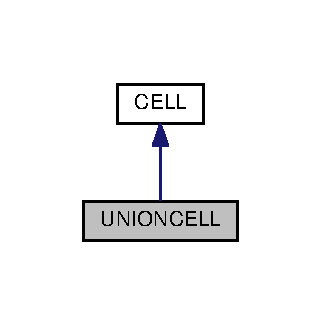
\includegraphics[width=154pt]{classUNIONCELL__inherit__graph}
\end{center}
\end{figure}


Collaboration diagram for U\+N\+I\+O\+N\+C\+E\+L\+L\+:\nopagebreak
\begin{figure}[H]
\begin{center}
\leavevmode
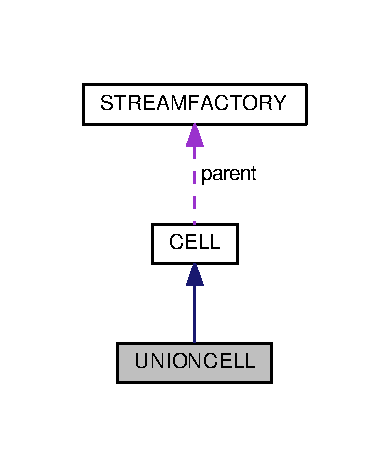
\includegraphics[width=187pt]{classUNIONCELL__coll__graph}
\end{center}
\end{figure}
\subsection*{Public Member Functions}
\begin{DoxyCompactItemize}
\item 
\hyperlink{classUNIONCELL_ad0a662c44a37238e6f948d2481a0438a}{U\+N\+I\+O\+N\+C\+E\+L\+L} (list$<$ \hyperlink{classPIPE}{P\+I\+P\+E} $\ast$ $>$ $\ast$inpipelist, uint dominantpipeid, list$<$ \hyperlink{classPIPE}{P\+I\+P\+E} $\ast$ $>$ $\ast$outpipelist, ushort count, \hyperlink{classSTREAMFACTORY}{S\+T\+R\+E\+A\+M\+F\+A\+C\+T\+O\+R\+Y} $\ast$parent, uint union\+\_\+policy)
\begin{DoxyCompactList}\small\item\em unioncell을 만드는 생성자. 코드세그먼트는 framework 내부적으로 정의되어 있는 것을 이용한다. \end{DoxyCompactList}\item 
virtual void \hyperlink{classUNIONCELL_ac57cb2a3f83bf219133a9d942c24f5aa}{make\+Worker} ()
\begin{DoxyCompactList}\small\item\em 워커를 만든다. \end{DoxyCompactList}\item 
virtual void $\ast$ \hyperlink{classUNIONCELL_a0179dad91d30e7bca318bb7e3b4a4995}{scheduling} (void $\ast$arg)
\begin{DoxyCompactList}\small\item\em 만든 워커를 실제로 스케줄링 하는 함수 \end{DoxyCompactList}\item 
list$<$ \hyperlink{classPIPE}{P\+I\+P\+E} $\ast$ $>$ $\ast$ \hyperlink{classUNIONCELL_a23ad55db09a70ba74f2fcf630def1c3f}{getinpipelist} ()
\begin{DoxyCompactList}\small\item\em cell에 연결된 inpipe list를 반환하는 함수 \end{DoxyCompactList}\item 
M\+E\+R\+G\+E\+\_\+\+F\+U\+N\+C \hyperlink{classUNIONCELL_a3ac189ca39d6445213365cadf9e21726}{getfunc} ()
\begin{DoxyCompactList}\small\item\em 코드 세그먼트를 반환하는 함수 \end{DoxyCompactList}\item 
pthread\+\_\+mutex\+\_\+t $\ast$ \hyperlink{classUNIONCELL_a42d955ed8ce559f41bd4837eda14a4ee}{getpipelock} ()
\begin{DoxyCompactList}\small\item\em input pipe들의 락을 반환하는 함수 \end{DoxyCompactList}\item 
uint \hyperlink{classUNIONCELL_abb9d6890717720d1472a97a8122beee1}{getdominantpipeid} ()
\begin{DoxyCompactList}\small\item\em dominantpipeid를 반환받는다. \end{DoxyCompactList}\item 
uint \hyperlink{classUNIONCELL_aac0488cf7d003881e4cfa45ce2055e36}{get\+Union\+Policy} ()
\begin{DoxyCompactList}\small\item\em union policy를 받는다. \end{DoxyCompactList}\end{DoxyCompactItemize}
\subsection*{Additional Inherited Members}


\subsection{Detailed Description}
cell의 기본 형태를 상속하고 M\+I\+S\+O의 형태를 갖고 있는 union cell이다. (processing cell이 아니다.) M\+I\+S\+O의 형태를 갖는다. 

cell의 기본 형태를 상속하고 M\+I\+S\+O의 형태를 갖고 있는 union cell이다. (processing cell이 아니다.) M\+I\+S\+O의 형태를 갖는다. 단순히 두개 이상의 튜플을 합쳐준다. 예를들어 하나의 튜플은 \mbox{[}int, char\mbox{]} 데이터를 갖고 있고 다른 하나의 튜플은 \mbox{[}char, char\mbox{]}를 갖고 있으면 합쳐지면 \mbox{[}int, char, char, char\mbox{]}의 튜플을 갖게 된다. \begin{DoxyAuthor}{Author}
ysmoon 
\end{DoxyAuthor}
\begin{DoxyDate}{Date}
2016-\/11-\/08 
\end{DoxyDate}
\begin{DoxyVersion}{Version}
0.\+0.\+1 
\end{DoxyVersion}


\subsection{Constructor \& Destructor Documentation}
\hypertarget{classUNIONCELL_ad0a662c44a37238e6f948d2481a0438a}{}\index{U\+N\+I\+O\+N\+C\+E\+L\+L@{U\+N\+I\+O\+N\+C\+E\+L\+L}!U\+N\+I\+O\+N\+C\+E\+L\+L@{U\+N\+I\+O\+N\+C\+E\+L\+L}}
\index{U\+N\+I\+O\+N\+C\+E\+L\+L@{U\+N\+I\+O\+N\+C\+E\+L\+L}!U\+N\+I\+O\+N\+C\+E\+L\+L@{U\+N\+I\+O\+N\+C\+E\+L\+L}}
\subsubsection[{U\+N\+I\+O\+N\+C\+E\+L\+L}]{\setlength{\rightskip}{0pt plus 5cm}U\+N\+I\+O\+N\+C\+E\+L\+L\+::\+U\+N\+I\+O\+N\+C\+E\+L\+L (
\begin{DoxyParamCaption}
\item[{list$<$ {\bf P\+I\+P\+E} $\ast$ $>$ $\ast$}]{inpipelist, }
\item[{uint}]{dominantpipeid, }
\item[{list$<$ {\bf P\+I\+P\+E} $\ast$ $>$ $\ast$}]{outpipelist, }
\item[{ushort}]{count, }
\item[{{\bf S\+T\+R\+E\+A\+M\+F\+A\+C\+T\+O\+R\+Y} $\ast$}]{parent, }
\item[{uint}]{union\+\_\+policy}
\end{DoxyParamCaption}
)}\label{classUNIONCELL_ad0a662c44a37238e6f948d2481a0438a}


unioncell을 만드는 생성자. 코드세그먼트는 framework 내부적으로 정의되어 있는 것을 이용한다. 

unioncell을 만드는 생성자. 코드세그먼트는 framework 내부적으로 정의되어 있는 것을 이용한다. 
\begin{DoxyParams}{Parameters}
{\em inpipelist} & cell에 대한 input pipe list이다. 깊은 복사로 넘어간다. 이후 파라미터로 들어온것은 필요 없으면 메모리 해제 해야 한다. \\
\hline
{\em dominantpipeid} & 두개 이상의 튜플을 합칠 때, 결과 튜플의 속성에 어떤 파이프에 있던 튜플 속성을 합칠 지 정의한다. 예를들어 1번파이프와 2번파이프가 연결되어 있고 dominantpipeid가 1번 파이프로 지정되면, 결과튜플은 항상 1번 파이프의 속성을 갖는다. \\
\hline
{\em outpipe} & cell에 대한 단일 output pipe이다. \\
\hline
{\em count} & cell에 들어있는 worker의 개수를 정의한다. worker는 단순히 두개 이상의 튜플을 합치는 일을 한다. \\
\hline
{\em parent} & cell이 속한 factory를 명시한다. \\
\hline
\end{DoxyParams}


\subsection{Member Function Documentation}
\hypertarget{classUNIONCELL_abb9d6890717720d1472a97a8122beee1}{}\index{U\+N\+I\+O\+N\+C\+E\+L\+L@{U\+N\+I\+O\+N\+C\+E\+L\+L}!getdominantpipeid@{getdominantpipeid}}
\index{getdominantpipeid@{getdominantpipeid}!U\+N\+I\+O\+N\+C\+E\+L\+L@{U\+N\+I\+O\+N\+C\+E\+L\+L}}
\subsubsection[{getdominantpipeid}]{\setlength{\rightskip}{0pt plus 5cm}uint U\+N\+I\+O\+N\+C\+E\+L\+L\+::getdominantpipeid (
\begin{DoxyParamCaption}
{}
\end{DoxyParamCaption}
)}\label{classUNIONCELL_abb9d6890717720d1472a97a8122beee1}


dominantpipeid를 반환받는다. 

dominantpipeid를 반환받는다. dominantpipeid는 두개 이상의 튜플을 합칠 때, 결과 튜플의 속성에 어떤 파이프에 있던 튜플 속성을 합칠 지 정의한다. 예를들어 1번파이프와 2번파이프가 연결되어 있고 dominantpipeid가 1번 파이프로 지정되면, 결과튜플은 항상 1번 파이프의 속성을 갖는다. \begin{DoxyReturn}{Returns}
dominantpipeid 
\end{DoxyReturn}
\hypertarget{classUNIONCELL_a3ac189ca39d6445213365cadf9e21726}{}\index{U\+N\+I\+O\+N\+C\+E\+L\+L@{U\+N\+I\+O\+N\+C\+E\+L\+L}!getfunc@{getfunc}}
\index{getfunc@{getfunc}!U\+N\+I\+O\+N\+C\+E\+L\+L@{U\+N\+I\+O\+N\+C\+E\+L\+L}}
\subsubsection[{getfunc}]{\setlength{\rightskip}{0pt plus 5cm}M\+E\+R\+G\+E\+\_\+\+F\+U\+N\+C U\+N\+I\+O\+N\+C\+E\+L\+L\+::getfunc (
\begin{DoxyParamCaption}
{}
\end{DoxyParamCaption}
)}\label{classUNIONCELL_a3ac189ca39d6445213365cadf9e21726}


코드 세그먼트를 반환하는 함수 

코드 세그먼트를 반환하는 함수. \begin{DoxyReturn}{Returns}
M\+E\+R\+G\+E\+\_\+\+F\+U\+N\+C로, T\+U\+P\+L\+E$\ast$ \hyperlink{UNIONCELL_8h_a6f5457bd2820312a229bf464f813198d}{merge(list$<$ T\+U\+P\+L\+E$\ast$ $>$$\ast$ tuplelist, uint dominantpipeid)} 함수 형태를 갖는 포인터를 반환한다. 
\end{DoxyReturn}
\hypertarget{classUNIONCELL_a23ad55db09a70ba74f2fcf630def1c3f}{}\index{U\+N\+I\+O\+N\+C\+E\+L\+L@{U\+N\+I\+O\+N\+C\+E\+L\+L}!getinpipelist@{getinpipelist}}
\index{getinpipelist@{getinpipelist}!U\+N\+I\+O\+N\+C\+E\+L\+L@{U\+N\+I\+O\+N\+C\+E\+L\+L}}
\subsubsection[{getinpipelist}]{\setlength{\rightskip}{0pt plus 5cm}list$<$ {\bf P\+I\+P\+E} $\ast$ $>$ $\ast$ U\+N\+I\+O\+N\+C\+E\+L\+L\+::getinpipelist (
\begin{DoxyParamCaption}
{}
\end{DoxyParamCaption}
)}\label{classUNIONCELL_a23ad55db09a70ba74f2fcf630def1c3f}


cell에 연결된 inpipe list를 반환하는 함수 

cell에 연결된 inpipe list를 반환하는 함수 \begin{DoxyReturn}{Returns}
list$<$\+P\+I\+P\+E$\ast$$>$$\ast$로써, 파이프 리스트 포인터를 반환받는다. 
\end{DoxyReturn}
\hypertarget{classUNIONCELL_a42d955ed8ce559f41bd4837eda14a4ee}{}\index{U\+N\+I\+O\+N\+C\+E\+L\+L@{U\+N\+I\+O\+N\+C\+E\+L\+L}!getpipelock@{getpipelock}}
\index{getpipelock@{getpipelock}!U\+N\+I\+O\+N\+C\+E\+L\+L@{U\+N\+I\+O\+N\+C\+E\+L\+L}}
\subsubsection[{getpipelock}]{\setlength{\rightskip}{0pt plus 5cm}pthread\+\_\+mutex\+\_\+t $\ast$ U\+N\+I\+O\+N\+C\+E\+L\+L\+::getpipelock (
\begin{DoxyParamCaption}
{}
\end{DoxyParamCaption}
)}\label{classUNIONCELL_a42d955ed8ce559f41bd4837eda14a4ee}


input pipe들의 락을 반환하는 함수 

input pipe들의 락을 반환하는 함수. unioncell은 워커가 두개 이상의 파이프에 접근을 하기 때문에, 관리 리스트등이 atomic operation을 제대로 수행하지 못해 오류가 날 수 있다. 그러므로 락을 걸어 보호한다. \begin{DoxyReturn}{Returns}
pthread\+\_\+mutex\+\_\+t$\ast$ 로써, 락의 포인터를 반환한다. 
\end{DoxyReturn}
\begin{DoxyRefDesc}{Todo}
\item[\hyperlink{todo__todo000007}{Todo}]pipe락을 없애는 방법이 있으면 없애기 \end{DoxyRefDesc}
\hypertarget{classUNIONCELL_aac0488cf7d003881e4cfa45ce2055e36}{}\index{U\+N\+I\+O\+N\+C\+E\+L\+L@{U\+N\+I\+O\+N\+C\+E\+L\+L}!get\+Union\+Policy@{get\+Union\+Policy}}
\index{get\+Union\+Policy@{get\+Union\+Policy}!U\+N\+I\+O\+N\+C\+E\+L\+L@{U\+N\+I\+O\+N\+C\+E\+L\+L}}
\subsubsection[{get\+Union\+Policy}]{\setlength{\rightskip}{0pt plus 5cm}uint U\+N\+I\+O\+N\+C\+E\+L\+L\+::get\+Union\+Policy (
\begin{DoxyParamCaption}
{}
\end{DoxyParamCaption}
)}\label{classUNIONCELL_aac0488cf7d003881e4cfa45ce2055e36}


union policy를 받는다. 

union policy를 받는다. P\+O\+L\+I\+C\+Y\+\_\+\+A\+L\+L\+R\+E\+A\+D\+Y, P\+O\+L\+I\+C\+Y\+\_\+\+P\+A\+R\+T\+I\+A\+L\+R\+E\+A\+D\+Y를 반환 \begin{DoxyReturn}{Returns}
P\+O\+L\+I\+C\+Y\+\_\+\+A\+L\+L\+R\+E\+A\+D\+Y(0), P\+O\+L\+I\+C\+Y\+\_\+\+P\+A\+R\+T\+I\+A\+L\+R\+E\+A\+D\+Y(1)를 반환 
\end{DoxyReturn}
\hypertarget{classUNIONCELL_ac57cb2a3f83bf219133a9d942c24f5aa}{}\index{U\+N\+I\+O\+N\+C\+E\+L\+L@{U\+N\+I\+O\+N\+C\+E\+L\+L}!make\+Worker@{make\+Worker}}
\index{make\+Worker@{make\+Worker}!U\+N\+I\+O\+N\+C\+E\+L\+L@{U\+N\+I\+O\+N\+C\+E\+L\+L}}
\subsubsection[{make\+Worker}]{\setlength{\rightskip}{0pt plus 5cm}void U\+N\+I\+O\+N\+C\+E\+L\+L\+::make\+Worker (
\begin{DoxyParamCaption}
{}
\end{DoxyParamCaption}
)\hspace{0.3cm}{\ttfamily [virtual]}}\label{classUNIONCELL_ac57cb2a3f83bf219133a9d942c24f5aa}


워커를 만든다. 

워커를 만든다. unioncell 생성자의 count에서 정의된 숫자만큼 합치는 기능을 수행하는 워커를 만든다. cell의 순수 가상 함수를 implementation한다. \begin{DoxyReturn}{Returns}
void 의미 없음 
\end{DoxyReturn}


Implements \hyperlink{classCELL_a1b048e8ac8cc57bcdff18bbcba6ed975}{C\+E\+L\+L}.

\hypertarget{classUNIONCELL_a0179dad91d30e7bca318bb7e3b4a4995}{}\index{U\+N\+I\+O\+N\+C\+E\+L\+L@{U\+N\+I\+O\+N\+C\+E\+L\+L}!scheduling@{scheduling}}
\index{scheduling@{scheduling}!U\+N\+I\+O\+N\+C\+E\+L\+L@{U\+N\+I\+O\+N\+C\+E\+L\+L}}
\subsubsection[{scheduling}]{\setlength{\rightskip}{0pt plus 5cm}void $\ast$ U\+N\+I\+O\+N\+C\+E\+L\+L\+::scheduling (
\begin{DoxyParamCaption}
\item[{void $\ast$}]{arg}
\end{DoxyParamCaption}
)\hspace{0.3cm}{\ttfamily [virtual]}}\label{classUNIONCELL_a0179dad91d30e7bca318bb7e3b4a4995}


만든 워커를 실제로 스케줄링 하는 함수 

워커를 실제로 스케줄링 하는 함수이다. cell의 scheduling\+\_\+wrapper에 의해 불린다. while문을 돌면서 iput pipe들을 풀링한다. \begin{DoxyReturn}{Returns}
void 의미 없음 
\end{DoxyReturn}
\begin{DoxyRefDesc}{Bug}
\item[\hyperlink{bug__bug000002}{Bug}]스케줄링에서 outpipe로 데이터를 넘길 때, pipe에 각각 데이터를 깊은복사를 해서 넘겨주어야 한다. \end{DoxyRefDesc}


Implements \hyperlink{classCELL_adcd2e66700a2c6f0cb234cbe63d2e10c}{C\+E\+L\+L}.



The documentation for this class was generated from the following files\+:\begin{DoxyCompactItemize}
\item 
include/\hyperlink{UNIONCELL_8h}{U\+N\+I\+O\+N\+C\+E\+L\+L.\+h}\item 
U\+N\+I\+O\+N\+C\+E\+L\+L.\+cpp\end{DoxyCompactItemize}

\hypertarget{classWORKER}{}\section{W\+O\+R\+K\+E\+R Class Reference}
\label{classWORKER}\index{W\+O\+R\+K\+E\+R@{W\+O\+R\+K\+E\+R}}
\subsection*{Public Member Functions}
\begin{DoxyCompactItemize}
\item 
\hypertarget{classWORKER_ae9ea2fc90f6cb11e7112f6b66b90f834}{}{\bfseries W\+O\+R\+K\+E\+R} (\hyperlink{classCELL}{C\+E\+L\+L} $\ast$parent)\label{classWORKER_ae9ea2fc90f6cb11e7112f6b66b90f834}

\item 
\hypertarget{classWORKER_ab7846a18291a8256d8834d5ce2cd2264}{}bool {\bfseries is\+Working} ()\label{classWORKER_ab7846a18291a8256d8834d5ce2cd2264}

\item 
\hypertarget{classWORKER_ac67e81ebc21a012b2ee0b486207b7b66}{}void {\bfseries create} ()\label{classWORKER_ac67e81ebc21a012b2ee0b486207b7b66}

\item 
\hypertarget{classWORKER_a4096ee44fb20e1d02708b04ee1536f0f}{}void {\bfseries wakeup} ()\label{classWORKER_a4096ee44fb20e1d02708b04ee1536f0f}

\item 
\hypertarget{classWORKER_a6aed2eee5acd22c3188305ae7e31b8d7}{}void {\bfseries sleep} ()\label{classWORKER_a6aed2eee5acd22c3188305ae7e31b8d7}

\item 
\hypertarget{classWORKER_a2153365418c1449448bd7ed0024540b8}{}\hyperlink{classCELL}{C\+E\+L\+L} $\ast$ {\bfseries get\+Parent\+C\+E\+L\+L} ()\label{classWORKER_a2153365418c1449448bd7ed0024540b8}

\end{DoxyCompactItemize}


The documentation for this class was generated from the following files\+:\begin{DoxyCompactItemize}
\item 
include/W\+O\+R\+K\+E\+R.\+h\item 
W\+O\+R\+K\+E\+R.\+cpp\end{DoxyCompactItemize}

\chapter{File Documentation}
\hypertarget{BASICCELL_8h}{}\section{include/\+B\+A\+S\+I\+C\+C\+E\+L\+L.h File Reference}
\label{BASICCELL_8h}\index{include/\+B\+A\+S\+I\+C\+C\+E\+L\+L.\+h@{include/\+B\+A\+S\+I\+C\+C\+E\+L\+L.\+h}}


processing cell의 basic cell을 정의해놓은 헤더  


{\ttfamily \#include $<$stdlib.\+h$>$}\\*
{\ttfamily \#include $<$list$>$}\\*
{\ttfamily \#include $<$functional$>$}\\*
{\ttfamily \#include $<$pthread.\+h$>$}\\*
{\ttfamily \#include \char`\"{}Functions.\+h\char`\"{}}\\*
{\ttfamily \#include \char`\"{}C\+E\+L\+L.\+h\char`\"{}}\\*
Include dependency graph for B\+A\+S\+I\+C\+C\+E\+L\+L.\+h\+:\nopagebreak
\begin{figure}[H]
\begin{center}
\leavevmode
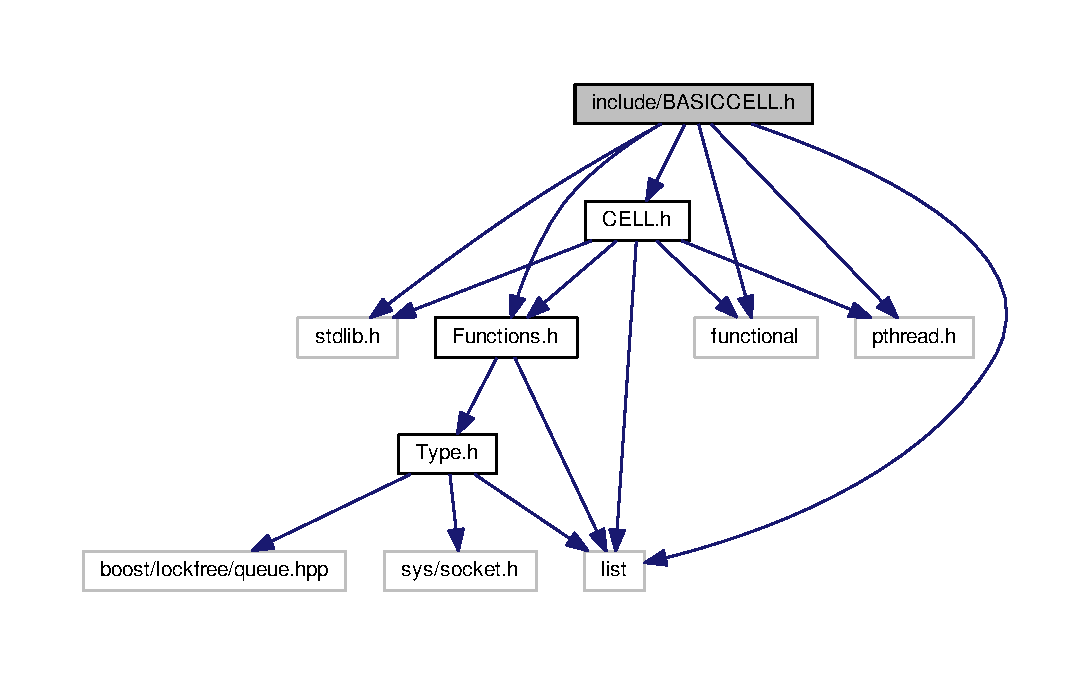
\includegraphics[width=350pt]{BASICCELL_8h__incl}
\end{center}
\end{figure}
\subsection*{Classes}
\begin{DoxyCompactItemize}
\item 
class \hyperlink{classBASICCELL}{B\+A\+S\+I\+C\+C\+E\+L\+L}
\begin{DoxyCompactList}\small\item\em cell의 기본 형태를 상속하고 S\+I\+S\+O의 형태를 갖고 있는 processing cell. 실제 processing의 유닛이다. \end{DoxyCompactList}\end{DoxyCompactItemize}


\subsection{Detailed Description}
processing cell의 basic cell을 정의해놓은 헤더 


\hypertarget{CELL_8h}{}\section{include/\+C\+E\+L\+L.h File Reference}
\label{CELL_8h}\index{include/\+C\+E\+L\+L.\+h@{include/\+C\+E\+L\+L.\+h}}


processing cell의 기본단위인 cell의 기본 형태를 정의해놓은 헤더  


{\ttfamily \#include $<$stdlib.\+h$>$}\\*
{\ttfamily \#include $<$list$>$}\\*
{\ttfamily \#include $<$functional$>$}\\*
{\ttfamily \#include $<$pthread.\+h$>$}\\*
{\ttfamily \#include \char`\"{}Functions.\+h\char`\"{}}\\*
Include dependency graph for C\+E\+L\+L.\+h\+:\nopagebreak
\begin{figure}[H]
\begin{center}
\leavevmode
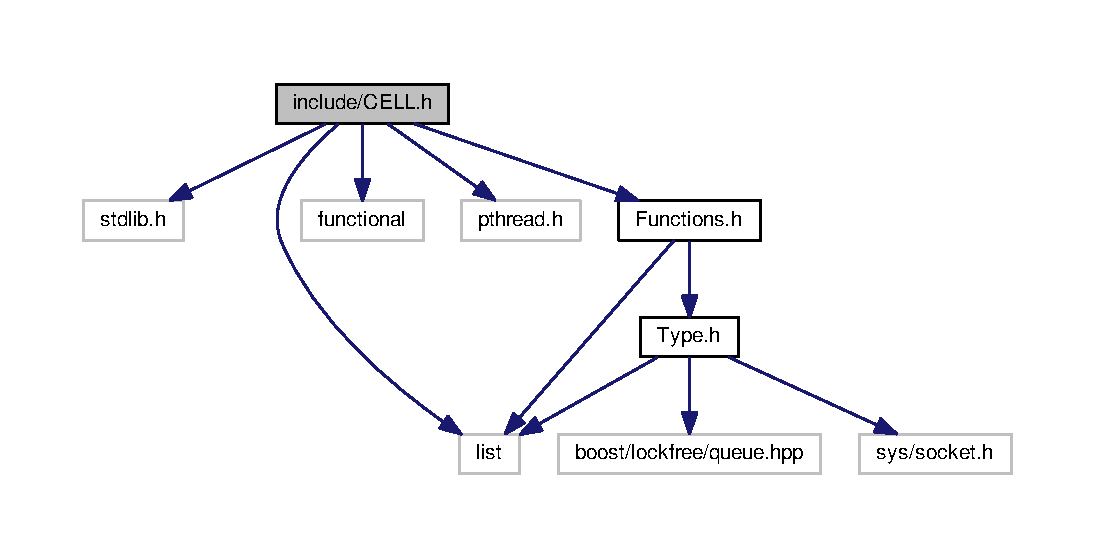
\includegraphics[width=350pt]{CELL_8h__incl}
\end{center}
\end{figure}
This graph shows which files directly or indirectly include this file\+:\nopagebreak
\begin{figure}[H]
\begin{center}
\leavevmode
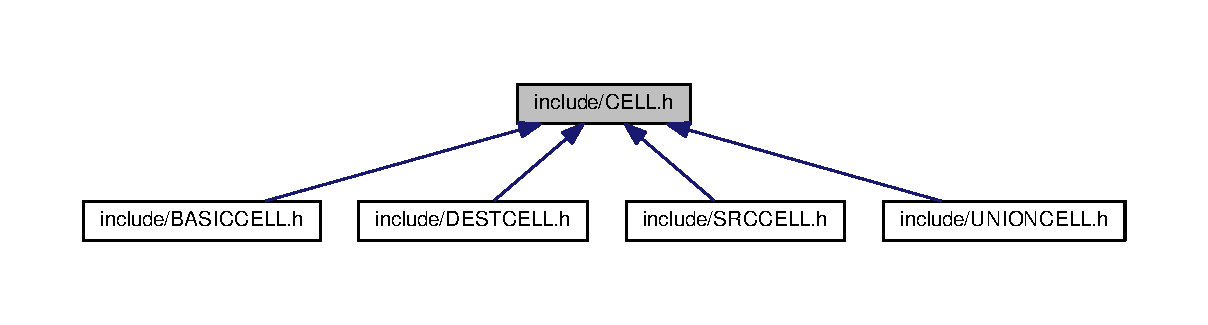
\includegraphics[width=350pt]{CELL_8h__dep__incl}
\end{center}
\end{figure}
\subsection*{Classes}
\begin{DoxyCompactItemize}
\item 
class \hyperlink{classCELL}{C\+E\+L\+L}
\begin{DoxyCompactList}\small\item\em processing cell의 기본 구현이 들어있는 클래스 \end{DoxyCompactList}\end{DoxyCompactItemize}
\subsection*{Macros}
\begin{DoxyCompactItemize}
\item 
\hypertarget{CELL_8h_a92636fc5211b846b5c36dd946d39b594}{}\#define {\bfseries S\+I\+S\+O}~0\label{CELL_8h_a92636fc5211b846b5c36dd946d39b594}

\item 
\hypertarget{CELL_8h_a7334c540878c8c4d801fd75ed9fd8063}{}\#define {\bfseries M\+I\+S\+O}~1\label{CELL_8h_a7334c540878c8c4d801fd75ed9fd8063}

\item 
\hypertarget{CELL_8h_a02cc6d026fad97c4a8c84675a0619d03}{}\#define {\bfseries S\+O}~2\label{CELL_8h_a02cc6d026fad97c4a8c84675a0619d03}

\item 
\hypertarget{CELL_8h_aa1be7844620ac7bffe73137a180aa044}{}\#define {\bfseries S\+I}~3\label{CELL_8h_aa1be7844620ac7bffe73137a180aa044}

\end{DoxyCompactItemize}


\subsection{Detailed Description}
processing cell의 기본단위인 cell의 기본 형태를 정의해놓은 헤더 


\hypertarget{DESTCELL_8h}{}\section{include/\+D\+E\+S\+T\+C\+E\+L\+L.h File Reference}
\label{DESTCELL_8h}\index{include/\+D\+E\+S\+T\+C\+E\+L\+L.\+h@{include/\+D\+E\+S\+T\+C\+E\+L\+L.\+h}}


destcell을 정의해놓은 헤더  


{\ttfamily \#include \char`\"{}C\+E\+L\+L.\+h\char`\"{}}\\*
{\ttfamily \#include $<$list$>$}\\*
{\ttfamily \#include $<$sys/socket.\+h$>$}\\*
{\ttfamily \#include $<$netinet/in.\+h$>$}\\*
{\ttfamily \#include $<$netdb.\+h$>$}\\*
{\ttfamily \#include $<$arpa/inet.\+h$>$}\\*
{\ttfamily \#include $<$string.\+h$>$}\\*
{\ttfamily \#include $<$pthread.\+h$>$}\\*
{\ttfamily \#include $<$deque$>$}\\*
Include dependency graph for D\+E\+S\+T\+C\+E\+L\+L.\+h\+:\nopagebreak
\begin{figure}[H]
\begin{center}
\leavevmode
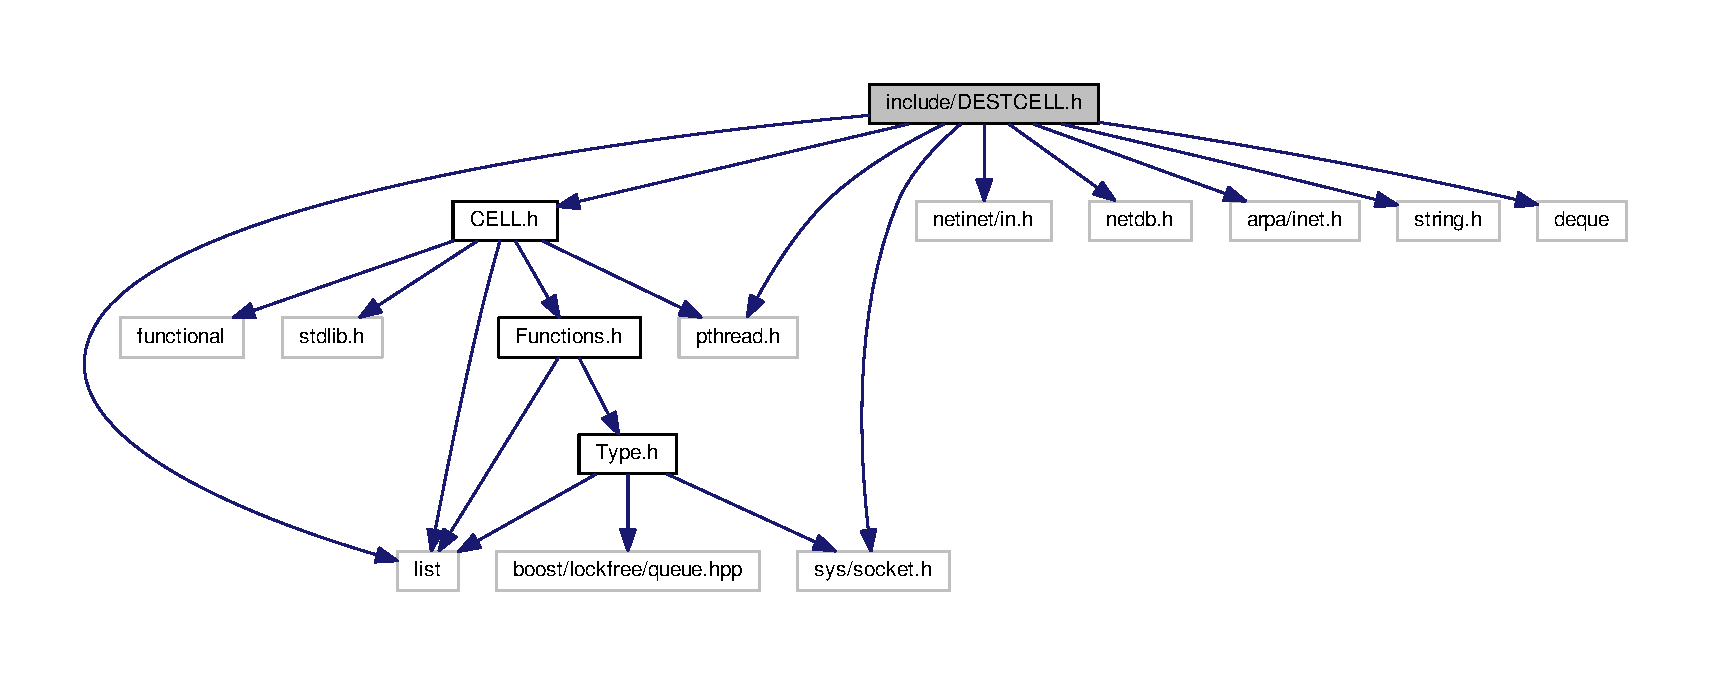
\includegraphics[width=350pt]{DESTCELL_8h__incl}
\end{center}
\end{figure}
\subsection*{Classes}
\begin{DoxyCompactItemize}
\item 
class \hyperlink{classDESTCELL}{D\+E\+S\+T\+C\+E\+L\+L}
\begin{DoxyCompactList}\small\item\em destcell을 정의해놓은 클래스. factory에서 나가는 데이터의 종말 지점이다. \end{DoxyCompactList}\end{DoxyCompactItemize}


\subsection{Detailed Description}
destcell을 정의해놓은 헤더 


\hypertarget{FACTORYBUILDER_8h}{}\section{include/\+F\+A\+C\+T\+O\+R\+Y\+B\+U\+I\+L\+D\+E\+R.h File Reference}
\label{FACTORYBUILDER_8h}\index{include/\+F\+A\+C\+T\+O\+R\+Y\+B\+U\+I\+L\+D\+E\+R.\+h@{include/\+F\+A\+C\+T\+O\+R\+Y\+B\+U\+I\+L\+D\+E\+R.\+h}}


factory를 만드는 툴인 factorybuilder를 정의해놓은 헤더  


{\ttfamily \#include $<$list$>$}\\*
{\ttfamily \#include $<$sys/types.\+h$>$}\\*
{\ttfamily \#include $<$boost/lockfree/queue.\+hpp$>$}\\*
{\ttfamily \#include $<$termios.\+h$>$}\\*
{\ttfamily \#include $<$unistd.\+h$>$}\\*
Include dependency graph for F\+A\+C\+T\+O\+R\+Y\+B\+U\+I\+L\+D\+E\+R.\+h\+:\nopagebreak
\begin{figure}[H]
\begin{center}
\leavevmode
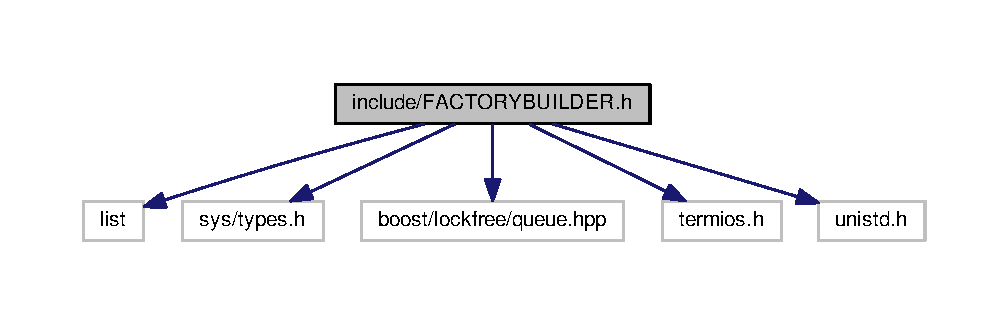
\includegraphics[width=350pt]{FACTORYBUILDER_8h__incl}
\end{center}
\end{figure}
\subsection*{Classes}
\begin{DoxyCompactItemize}
\item 
class \hyperlink{classFACTORYBUILDER}{F\+A\+C\+T\+O\+R\+Y\+B\+U\+I\+L\+D\+E\+R}
\begin{DoxyCompactList}\small\item\em factory builder를 만든다. \end{DoxyCompactList}\end{DoxyCompactItemize}
\subsection*{Variables}
\begin{DoxyCompactItemize}
\item 
\hypertarget{FACTORYBUILDER_8h_aa4938e9f11ff8ba45797bc2687621c9b}{}\hyperlink{classFACTORYBUILDER}{F\+A\+C\+T\+O\+R\+Y\+B\+U\+I\+L\+D\+E\+R} {\bfseries factorymanager}\label{FACTORYBUILDER_8h_aa4938e9f11ff8ba45797bc2687621c9b}

\end{DoxyCompactItemize}


\subsection{Detailed Description}
factory를 만드는 툴인 factorybuilder를 정의해놓은 헤더 


\hypertarget{SRCCELL_8h}{}\section{include/\+S\+R\+C\+C\+E\+L\+L.h File Reference}
\label{SRCCELL_8h}\index{include/\+S\+R\+C\+C\+E\+L\+L.\+h@{include/\+S\+R\+C\+C\+E\+L\+L.\+h}}


srccell을 정의해놓은 헤더  


{\ttfamily \#include \char`\"{}C\+E\+L\+L.\+h\char`\"{}}\\*
{\ttfamily \#include $<$list$>$}\\*
{\ttfamily \#include $<$sys/socket.\+h$>$}\\*
{\ttfamily \#include $<$netinet/in.\+h$>$}\\*
{\ttfamily \#include $<$netdb.\+h$>$}\\*
{\ttfamily \#include $<$arpa/inet.\+h$>$}\\*
{\ttfamily \#include $<$string.\+h$>$}\\*
{\ttfamily \#include $<$pthread.\+h$>$}\\*
{\ttfamily \#include $<$deque$>$}\\*
Include dependency graph for S\+R\+C\+C\+E\+L\+L.\+h\+:\nopagebreak
\begin{figure}[H]
\begin{center}
\leavevmode
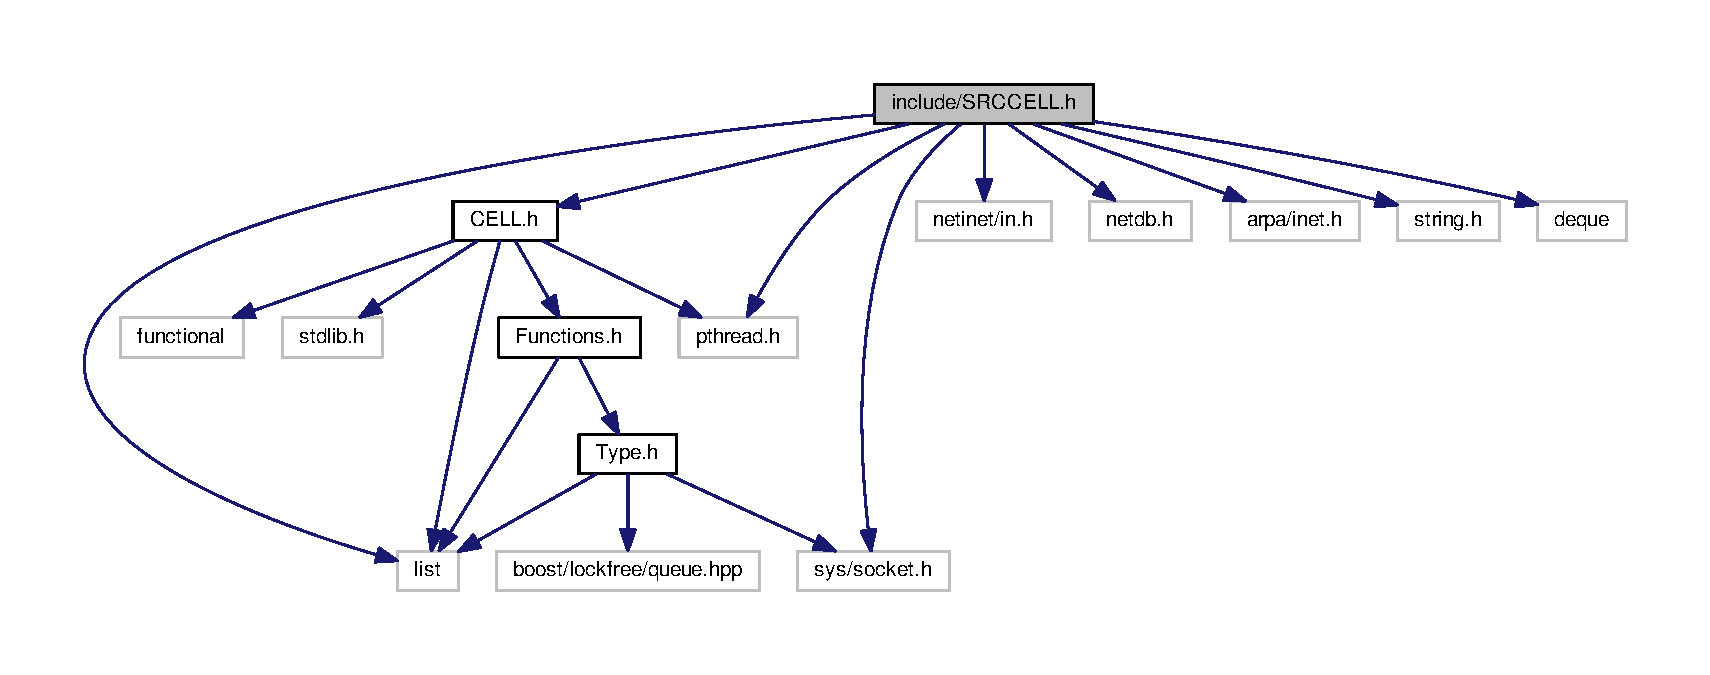
\includegraphics[width=350pt]{SRCCELL_8h__incl}
\end{center}
\end{figure}
\subsection*{Classes}
\begin{DoxyCompactItemize}
\item 
class \hyperlink{classSRCCELL}{S\+R\+C\+C\+E\+L\+L}
\begin{DoxyCompactList}\small\item\em srccell을 정의해놓은 클래스. factory로 들어오는 데이터의 시작 지점이다. cell의 형태를 상속하며 S\+O의 형태를 갖는다. \end{DoxyCompactList}\end{DoxyCompactItemize}


\subsection{Detailed Description}
srccell을 정의해놓은 헤더 


\hypertarget{TUPLE_8h}{}\section{include/\+T\+U\+P\+L\+E.h File Reference}
\label{TUPLE_8h}\index{include/\+T\+U\+P\+L\+E.\+h@{include/\+T\+U\+P\+L\+E.\+h}}


data의 교환단위인 tuple을 정의해놓은 헤더  


{\ttfamily \#include \char`\"{}Type.\+h\char`\"{}}\\*
{\ttfamily \#include $<$string.\+h$>$}\\*
{\ttfamily \#include $<$netinet/in.\+h$>$}\\*
Include dependency graph for T\+U\+P\+L\+E.\+h\+:\nopagebreak
\begin{figure}[H]
\begin{center}
\leavevmode
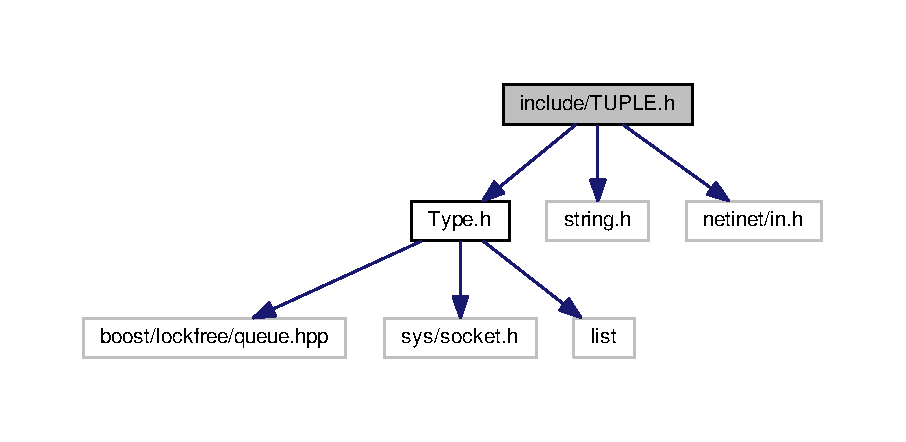
\includegraphics[width=350pt]{TUPLE_8h__incl}
\end{center}
\end{figure}
\subsection*{Classes}
\begin{DoxyCompactItemize}
\item 
class \hyperlink{classTUPLE}{T\+U\+P\+L\+E}
\begin{DoxyCompactList}\small\item\em data의 교환단위인 tuple을 정의한 클래스이다. \end{DoxyCompactList}\end{DoxyCompactItemize}
\subsection*{Typedefs}
\begin{DoxyCompactItemize}
\item 
\hypertarget{TUPLE_8h_ab95f123a6c9bcfee6a343170ef8c5f69}{}typedef unsigned short {\bfseries ushort}\label{TUPLE_8h_ab95f123a6c9bcfee6a343170ef8c5f69}

\item 
\hypertarget{TUPLE_8h_a65f85814a8290f9797005d3b28e7e5fc}{}typedef unsigned char {\bfseries uchar}\label{TUPLE_8h_a65f85814a8290f9797005d3b28e7e5fc}

\end{DoxyCompactItemize}


\subsection{Detailed Description}
data의 교환단위인 tuple을 정의해놓은 헤더 


\hypertarget{UNIONCELL_8h}{}\section{include/\+U\+N\+I\+O\+N\+C\+E\+L\+L.h File Reference}
\label{UNIONCELL_8h}\index{include/\+U\+N\+I\+O\+N\+C\+E\+L\+L.\+h@{include/\+U\+N\+I\+O\+N\+C\+E\+L\+L.\+h}}


두개 이상의 tuple을 합쳐주는 cell  


{\ttfamily \#include $<$stdlib.\+h$>$}\\*
{\ttfamily \#include $<$list$>$}\\*
{\ttfamily \#include $<$functional$>$}\\*
{\ttfamily \#include $<$pthread.\+h$>$}\\*
{\ttfamily \#include \char`\"{}Functions.\+h\char`\"{}}\\*
{\ttfamily \#include \char`\"{}C\+E\+L\+L.\+h\char`\"{}}\\*
Include dependency graph for U\+N\+I\+O\+N\+C\+E\+L\+L.\+h\+:\nopagebreak
\begin{figure}[H]
\begin{center}
\leavevmode
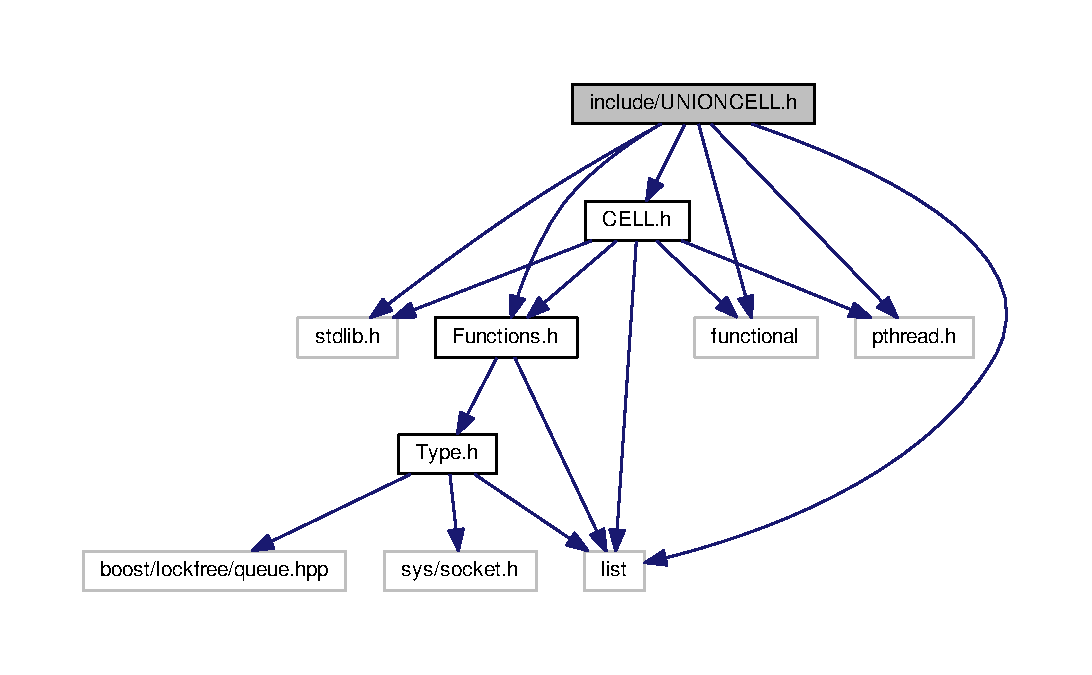
\includegraphics[width=350pt]{UNIONCELL_8h__incl}
\end{center}
\end{figure}
\subsection*{Classes}
\begin{DoxyCompactItemize}
\item 
class \hyperlink{classUNIONCELL}{U\+N\+I\+O\+N\+C\+E\+L\+L}
\begin{DoxyCompactList}\small\item\em cell의 기본 형태를 상속하고 M\+I\+S\+O의 형태를 갖고 있는 union cell이다. (processing cell이 아니다.) M\+I\+S\+O의 형태를 갖는다. \end{DoxyCompactList}\end{DoxyCompactItemize}
\subsection*{Macros}
\begin{DoxyCompactItemize}
\item 
\hypertarget{UNIONCELL_8h_afd95b62b61000ed5fc3e8517a33d9092}{}\#define {\bfseries P\+O\+L\+I\+C\+Y\+\_\+\+A\+L\+L\+R\+E\+A\+D\+Y}~0\label{UNIONCELL_8h_afd95b62b61000ed5fc3e8517a33d9092}

\item 
\hypertarget{UNIONCELL_8h_aaff08d419f716fc12722c8bbe8a4bc4b}{}\#define {\bfseries P\+O\+L\+I\+C\+Y\+\_\+\+P\+A\+R\+T\+I\+A\+L\+R\+E\+A\+D\+Y}~1\label{UNIONCELL_8h_aaff08d419f716fc12722c8bbe8a4bc4b}

\end{DoxyCompactItemize}
\subsection*{Functions}
\begin{DoxyCompactItemize}
\item 
\hyperlink{classTUPLE}{T\+U\+P\+L\+E} $\ast$ \hyperlink{UNIONCELL_8h_a6f5457bd2820312a229bf464f813198d}{merge} (list$<$ \hyperlink{classTUPLE}{T\+U\+P\+L\+E} $\ast$ $>$ $\ast$tuplelist, uint dominantpipeid)
\begin{DoxyCompactList}\small\item\em 두개 이상의 튜플을 merge를 수행하는 내부 로직 \end{DoxyCompactList}\end{DoxyCompactItemize}


\subsection{Detailed Description}
두개 이상의 tuple을 합쳐주는 cell 



\subsection{Function Documentation}
\hypertarget{UNIONCELL_8h_a6f5457bd2820312a229bf464f813198d}{}\index{U\+N\+I\+O\+N\+C\+E\+L\+L.\+h@{U\+N\+I\+O\+N\+C\+E\+L\+L.\+h}!merge@{merge}}
\index{merge@{merge}!U\+N\+I\+O\+N\+C\+E\+L\+L.\+h@{U\+N\+I\+O\+N\+C\+E\+L\+L.\+h}}
\subsubsection[{merge}]{\setlength{\rightskip}{0pt plus 5cm}{\bf T\+U\+P\+L\+E}$\ast$ merge (
\begin{DoxyParamCaption}
\item[{list$<$ {\bf T\+U\+P\+L\+E} $\ast$ $>$ $\ast$}]{tuplelist, }
\item[{uint}]{dominantpipeid}
\end{DoxyParamCaption}
)}\label{UNIONCELL_8h_a6f5457bd2820312a229bf464f813198d}


두개 이상의 튜플을 merge를 수행하는 내부 로직 

두개 이상의 튜플을 merge하는 내부 로직이다. 다수의 튜플은 리스트 형태로 들어가며, 또한 결과 튜플의 속성을 정의하기 위한 dominantpipeid가 필요하다. \begin{DoxyReturn}{Returns}
T\+U\+P\+L\+E$\ast$로써, 하나의 튜플 포인터를 반환한다. 
\end{DoxyReturn}

%--- End generated contents ---

% Index
\backmatter
\newpage
\phantomsection
\clearemptydoublepage
\addcontentsline{toc}{chapter}{Index}
\printindex

\end{document}
